%  LaTeX support: latex@mdpi.com
%  For support, please attach all files needed for compiling as well as the log file, and specify your operating system, LaTeX version, and LaTeX editor.

%=================================================================
\documentclass[technologies,article,submit,pdftex,moreauthors]{Definitions/mdpi}

%--------------------
% Class Options:
%--------------------

%=================================================================
% MDPI internal commands - do not modify
\firstpage{1}
\makeatletter
\setcounter{page}{\@firstpage}
\makeatother
\pubvolume{1}
\issuenum{1}
\articlenumber{0}
\pubyear{2026}
\copyrightyear{2026}
\datereceived{}
\daterevised{}
\dateaccepted{}
\datepublished{}

%=================================================================
% Submission target: MDPI Technologies
% Version 3 (2026-08-14/15). Base scaffolding (class, packages, MDPI-specific
% macros, section structure) copied from main_mdpi_v2.tex, which was itself
% pandoc-converted from main.md at the v2 stage -- this file was NOT freshly
% regenerated from Markdown via pandoc. Instead: main_mdpi_v3.md was diffed
% against main.md, and every content change (2026-08-13 consensus review's
% Priority 1-3 items, the SQuaD static-analysis enrichment, the TravisTorrent
% test-duration robustness check, the Future Work roadmap, etc.) was manually
% translated into the corresponding LaTeX edit here, hunk by hunk, to preserve
% the hand-tuned table/figure/adjustwidth formatting a fresh pandoc pass would
% have discarded. Section numbering uses real \label{}/\ref{} auto-numbering
% throughout. main_mdpi_v2.tex/.pdf and main.md are frozen and archived at
% paper-work/archive/superseded_drafts/; main_mdpi.tex (the original
% 2026-08-08 review round) predates both and was never itself overwritten.
%=================================================================

%=================================================================
% Add packages and commands
\usepackage{algorithm}
\usepackage{algpseudocode}
\usepackage{amsmath}
\usepackage{amssymb}
\usepackage{booktabs}
\usepackage{multirow}

% pandoc-generated body uses \tightlist for compact itemize/enumerate lists
\providecommand{\tightlist}{%
  \setlength{\itemsep}{0pt}\setlength{\parskip}{0pt}}

%=================================================================
% Full title of the paper (Capitalized)
\Title{PRESTO: A Machine Learning Framework for Predicting Software System Performance Using SDLC Metrics}

% Author Orchid ID: enter ID or remove command
\newcommand{\orcidauthorA}{0009-0009-9419-1015}
\newcommand{\orcidauthorB}{0009-0007-2638-1592}
\newcommand{\orcidauthorC}{0000-0002-0717-5888}

% Authors, for the paper (add full first names)
\Author{Amit J Rangari $^{1}$\orcidA{}, Lalit Narayan Mishra $^{2}$\orcidB{} and Biswaranjan Senapati $^{3,}$*\orcidC{}}

% MDPI internal command: Authors, for metadata in PDF
\AuthorNames{Amit J Rangari, Lalit Narayan Mishra and Biswaranjan Senapati}

\address{%
$^{1}$ \quad JPMorgan Chase, Atlanta, GA 30326, USA; amitrangari@ieee.org\\
$^{2}$ \quad Lowe's Companies Inc., Mooresville, NC 28117, USA; Lnm8910@gmail.com\\
$^{3}$ \quad Department of Computer Science, University of Arkansas at Little Rock (UALR), Little Rock, AR 72204, USA; bsenapati@ualr.edu
}

\corres{Correspondence: bsenapati@ualr.edu}

% Abstract (Do not insert blank lines, i.e. \\)
\abstract{How well can you predict production performance from development process data alone? Modern DevOps pipelines record 164 metrics across eight SDLC phases, yet no public dataset links these signals to runtime outcomes. We built PRESTO and a Gaussian copula-based synthetic data generator, to be released as a public benchmark upon acceptance. Across three enterprise-domain synthetic datasets, the best model achieved \(R^2 = 0.26\)--\(0.36\) using only SDLC process features; a target-correlation ablation shows this largely reflects recovery of the generator's specified structure, so the synthetic domains alone are not evidence of genuine signal. Adding historical uptime features inflated \(R^2\) to \(0.95\), and roughly 72\% of that gain is autoregressive persistence rather than process signal. Tree-based ensembles outperformed \emph{untuned} linear models; tuned linear models were competitive or better in 2 of 3 domains. Testing infrastructure availability was the strongest synthetic-domain predictor, outweighing code quality roughly 11:1; real-world TravisTorrent data is directionally consistent (Test-phase features rank \#1 in 5 of 7 projects), but a robustness check excluding a definitionally-circular test-duration feature drops every project's holdout \(R^2\) to negative, so this should be read as a weak, feature-ranking-only signal, not confirmation. We introduce Phase-Aware Recursive Feature Elimination, which guarantees cross-phase coverage but does not reliably beat simpler baselines. Four independent real-world datasets, now with bootstrap confidence intervals: TravisTorrent (\(R^2=0.475\) best of seven, median \(0.005\)), Mozilla Perfherder (\(R^2=0.17\)--\(0.91\), autoregressive persistence), GHALogs (\(R^2\approx0.11\), zero leakage risk, significant for all five models, \(n=28{,}443\)), and SQuaD (\(R^2=0.402\) defect-fix, our strongest point estimate but \emph{not} significant -- enriching with real static-analysis code-quality features raises it to \(0.483\) and narrows the CI to a near-miss \([-0.037, 0.738]\), still not significant; \(R^2=0.245\) CVE-count, weaker but significant). GHALogs and SQuaD's CVE-count result are what actually license a confirmatory claim: SDLC process signals carry genuine, transferable predictive value, though not uniformly across every real-world dataset examined.}

% Keywords
\keyword{continuous integration; DevOps; feature engineering; gradient boosting; machine learning; performance testing; SDLC metrics; software performance prediction; software quality}

%%%%%%%%%%%%%%%%%%%%%%%%%%%%%%%%%%%%%%%%%%
\begin{document}

\begin{figure}[H]
\begin{adjustwidth}{-\extralength}{0cm}
\centering
\centering
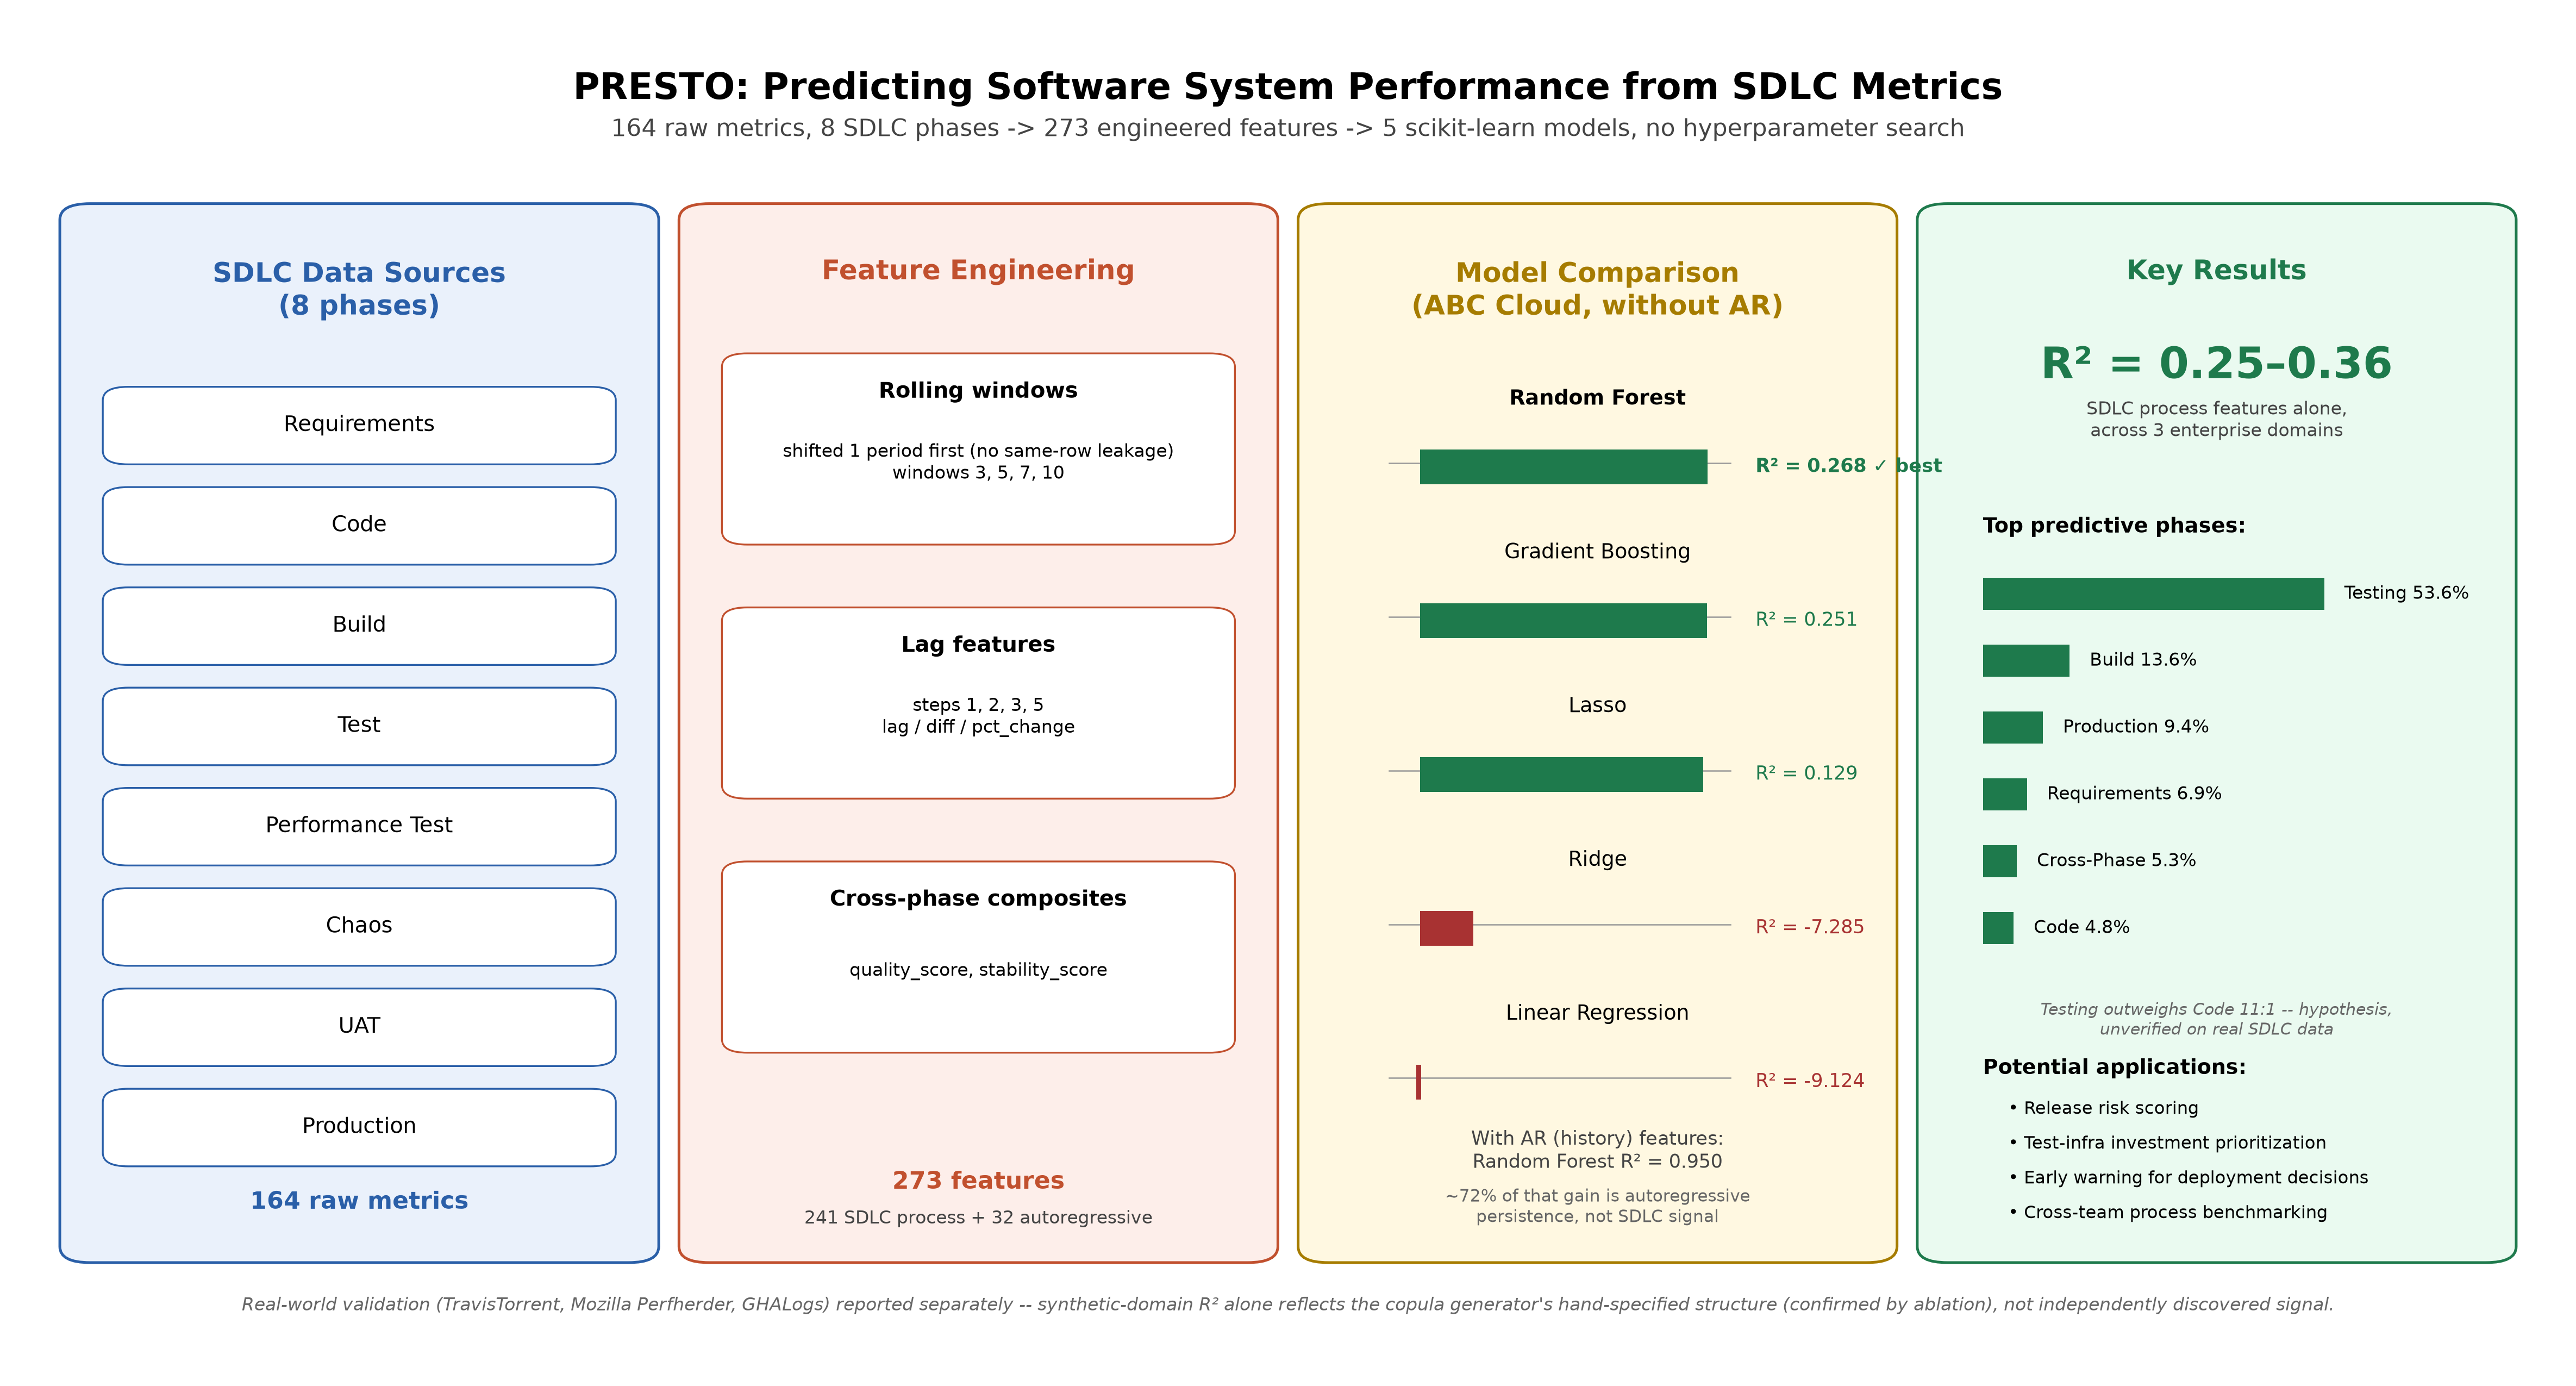
\includegraphics[width=\fulllength]{images/00-Graphical-Abstract.png}
\caption{Graphical Abstract. PRESTO framework overview: 164 SDLC metrics
from eight phases are transformed into 273 engineered features (241
SDLC process features plus 32 autoregressive) via
rolling windows, lag features, cross-phase interactions, and trend
derivatives. Five regression models are compared by holdout \(R^2\)
(5-fold \texttt{TimeSeriesSplit} CV also reported, but not used for
model selection -- see the pre-declared Model-Selection Rule,
Section~\ref{sec:exp_setup_validation}) across 170 releases spanning 5 years. Random Forest
achieves the best holdout \(R^2\) of 0.268 using only SDLC process
features without autoregressive (AR) features.\label{fig:graphical_abstract}}
\end{adjustwidth}
\end{figure}

%%%%%%%%%%%%%%%%%%%%%%%%%%%%%%%%%%%%%%%%%%
\section{Introduction}\label{sec:introduction}

Enterprise software teams ship code faster than ever, yet performance
validation remains the slowest gate in the deployment pipeline.
Organizations face the core challenge of balancing delivery speed with
thorough performance validation. Traditional performance testing often
slows deployment pipelines due to the extended duration required for
full-cycle load, stress, and endurance testing. Therefore, the central
thesis of this work is that shift-left testing principles can be
extended beyond functional testing to performance prediction: using
Software Development Lifecycle (SDLC) metrics, machine learning, and
historical performance data can enhance performance prediction, enabling
faster insights and risk management without compromising on quality or
reliability.

\subsection{Problem Context}\label{sec:problem_context}

As DevOps adoption accelerates and microservices replace monolithic
architectures, enterprise systems generate rich telemetry across every
phase of the software lifecycle. A cloud platform with hundreds of
microservices or a CRM system operated by dozens of teams produces
thousands of measurable signals per release cycle, from requirements
traceability scores through build pipeline metrics to production uptime
figures. Despite this telemetry abundance, performance prediction
remains largely disconnected from development process data. Most
approaches rely on post-deployment monitoring or pre-release load
testing, leaving the SDLC metrics pipeline untapped as a predictive
resource.

Current performance testing methodologies have several limitations.
First, feedback is often delayed, which conflicts with agile development
principles. Second, full testing is costly and impractical for every
minor change, resulting in incomplete insights during deployment
decision-making. Third, traditional approaches lack proactive issue
prediction: teams discover SLO breaches only after deployment, when the
blast radius has already expanded to customer-facing traffic. This
reactive posture is especially costly in microservice architectures
where a single degraded service can cascade across dependent consumers.

\subsection{Opportunity and Approach}\label{sec:opportunity}

The emergence of modern SDLC toolchains has created a new opportunity to
advance performance prediction through data-driven approaches. Modern
development environments capture detailed metrics across eight distinct
phases:

\begin{enumerate}
\def\labelenumi{\arabic{enumi}.}
\item
  \textbf{Requirements analysis}: Gathering and specifying what the
  system should do
\item
  \textbf{Code development}: Writing the underlying software
\item
  \textbf{Build processes}: Converting source code into executable
  programs
\item
  \textbf{Testing execution}: Running tests on the software
\item
  \textbf{Performance validation}: Specialist tests to verify system
  speed and responsiveness
\item
  \textbf{User acceptance testing (UAT)}: Tests by actual users to check
  if requirements are met
\item
  \textbf{Chaos engineering}: Intentional experimentation by introducing
  failures to test system resilience
\item
  \textbf{Production deployment}: Launching finalized software into its
  operational environment
\end{enumerate}

Our analysis of enterprise-scale development projects reveals that 164
distinct metrics are routinely collected across these phases. These
metrics include requirements stability indices (measures of changes in
requirements), code quality indicators (such as defect rates or
complexity), build success rates (proportion of successful builds), test
coverage metrics (how much of the code is tested), performance
benchmarks (quantifiable measures of speed or efficiency), user
satisfaction scores, resilience measurements (system ability to handle
disruptions), and production health indicators (measures of system
stability in live environments).

The sheer volume of these metrics enables machine learning performance
prediction. By tracking SDLC patterns from releases, models can identify
early indicators of potential problems for teams to address before
deployment. These systems bridge rapid development and performance
checks, offering feedback on code changes.

\subsection{Research Questions}\label{sec:research_questions}

This work addresses the following research questions:

\textbf{RQ1:} To what extent can SDLC metrics predict system
performance? (answered in Section~\ref{sec:model_perf})

\begin{itemize}
\tightlist
\item
  \emph{Operationalization}: We assess prediction accuracy using
  \(R^2\), Mean Absolute Error (MAE), and Root Mean Squared Error
  (RMSE). We distinguish between SDLC-only predictive signal and
  temporal autocorrelation of the target variable.
\end{itemize}

\textbf{RQ2:} Which SDLC phases and metrics are most predictive of
system performance? (answered in
Section~\ref{sec:feature_importance})

\begin{itemize}
\tightlist
\item
  \emph{Operationalization}: We analyze feature importance rankings and
  phase-level contribution percentages.
\end{itemize}

\textbf{RQ3:} How do different machine learning algorithms compare for
SDLC-based performance prediction? (answered in
Sections~\ref{sec:model_perf}
and~\ref{sec:model_char})

\begin{itemize}
\tightlist
\item
  \emph{Operationalization}: We evaluate five algorithms (Linear
  Regression, Ridge, Lasso, Random Forest, Gradient Boosting) using
  consistent validation protocols.
\end{itemize}

\textbf{RQ4:} What factors influence the accuracy of SDLC-based
performance predictions? (answered in
Section~\ref{sec:rq4_factors})

\begin{itemize}
\tightlist
\item
  \emph{Operationalization}: We examine temporal dependencies,
  cross-phase interactions, release characteristics, and system
  evolution impacts.
\end{itemize}

\subsection{Contributions}\label{sec:contributions}

The framework benefits organizations by potentially reducing deployment
risk, accelerating releases, focusing testing efforts, and preventing
customer-impacting problems. We propose PRESTO (Performance REgression
from Software development Telemetry and Operations), a performance
prediction framework driven by multi-phase SDLC metrics. By collecting
and analyzing data from each lifecycle phase, the framework supports our
key argument: SDLC metrics, when combined with machine learning, may
enable proactive performance forecasting.

We validate this approach with three synthetic datasets reflecting
enterprise domains: a five-year cloud platform (170 releases), a
CRM/SaaS system (200 releases), and a payment processor (150 releases),
demonstrating applicability across different application contexts.
Table~\ref{tab:summary_results} summarizes PRESTO's key results
across all evaluation domains.

{\def\LTcaptype{none} % do not increment counter
\begin{table}[H]
\centering
\caption{Summary of PRESTO's key results across all evaluation domains.\label{tab:summary_results}}
\begin{tabular}{@{}lllll@{}}
\toprule
\textbf{Domain} & \textbf{Releases} & \textbf{Best Model} &
\textbf{\(R^2\)} & \textbf{RMSE} \\
\midrule
ABC Cloud Provider & 170 & Random Forest & 0.268 & 0.597 \\
Card Payment Proc. & 150 & Lasso / RF & 0.362 & 1.126 \\
XYZ Sales Force & 200 & Random Forest & 0.255 & 0.778 \\
TravisTorrent (real) & 7 projects & Linear Regression & 0.475 & -- \\
\bottomrule
\end{tabular}
\end{table}
}

Our contributions advance software performance prediction by:

\begin{enumerate}
\def\labelenumi{\arabic{enumi}.}
\item
  \textbf{Operationalizing PRESTO, a unified SDLC metric collection and
  standardization framework}, enabling full-lifecycle analysis that
  integrates development process indicators with performance prediction.
\item
  \textbf{Shifting prediction left: using 241 features engineered from
  pre-deployment SDLC metrics} (test pass rates, build stability,
  requirements traceability) to predict production uptime before
  deployment, providing risk signals earlier than canary deployments can
  surface them.
\item
  \textbf{Developing a reproducible Gaussian copula-based synthetic data
  generator} that produces 164 SDLC metrics across eight phases,
  calibrated to DORA 2024 benchmarks, released as the first public
  benchmark for SDLC-to-performance prediction.
\item
  \textbf{Establishing honest baselines} (Section~\ref{sec:model_perf}): Random Forest
  achieves \(R^2 = 0.268\) using only SDLC process features on the
  primary domain, 0.255--0.362 across three enterprise domains (Section~\ref{sec:cross_domain}), beating naive baselines (\(R^2 = -0.43\) to \(-1.64\)) while
  transparently reporting the gap between with-AR-features and
  without-AR-features performance.
\item
  \textbf{Quantifying autoregressive-feature dependence in SDLC
  performance prediction} (Section~\ref{sec:leakage}): we show that
  \textasciitilde72\% of Random Forest's apparent predictive power
  (\(R^2\) dropping from 0.950 to 0.268) stems from autoregressive
  persistence, not genuine SDLC process signal -- and provide direct
  evidence (a controlled bug-fix comparison) that this AR-dependence is
  a real property of the data, not an artifact of a since-fixed same-row
  leakage bug.
\item
  \textbf{Identifying that testing infrastructure metrics} (Section~\ref{sec:feature_importance}): test environment availability at 42.9\% and test pass rate at
  10.6\% are the strongest SDLC predictors of production performance in
  this synthetic design, outweighing code quality metrics by roughly
  11:1. The original submission reported this as contradicted by our own
  TravisTorrent results, where repository age was claimed to be the most
  consistently predictive feature instead; recomputing feature
  importance under the reimplemented TravisTorrent adapter reverses that claim
  (Section~\ref{sec:travistorrent}) -- repository age leads 0 of 7 projects, while
  Test-phase metrics lead 5 of 7. This qualitative ranking is directionally
  consistent with, not contradicting, this synthetic-domain finding, but a
  robustness check excluding the one Test-phase feature that is
  definitionally part of the build-duration target
  (\texttt{tr\_\allowbreak log\_\allowbreak testduration}) shows the \emph{quantitative} signal was doing
  most of the work: with it excluded, every one of the 7 projects'
  best-model holdout \(R^2\) turns negative, so TravisTorrent no longer
  demonstrates real-world predictive power for any project, even though
  the surviving feature ranking still points the same direction. The underlying
  inter-metric correlations are also hand-specified in the copula
  generator's configuration rather than independently emergent (Section~\ref{sec:internal_validity}), so this synthetic-domain result should still be read as a
  hypothesis rather than independently validated, and the real-data picture
  is a weak, partial corroboration at best -- not a resolved contradiction.
\item
  \textbf{Providing a deployment-ready continuous learning framework}
  with drift detection (PSI, KS tests) and automated retraining triggers
  for production SDLC prediction systems.
\item
  \textbf{Proposing PA-RFE (Phase-Aware Recursive Feature Elimination)}
  (Algorithm~\ref{alg:parfe},
  Section~\ref{sec:parfe_results}), a new feature
  selection algorithm that reduces dimensionality while guaranteeing
  representation from all 8 SDLC phases. Reimplemented from the paper's
  own pseudocode after the original implementation was found to be
  missing from the reproducibility package (Section~\ref{sec:parfe_results}): the
  phase-coverage guarantee holds on all three domains, but the original
  claim of competitive or best test-set predictive accuracy does not
  survive reimplementation -- PA-RFE avoids standard RFE's collapse on 1
  of 3 domains, not 2, and is outperformed by a simple SelectKBest
  baseline on the primary domain.
\item
  \textbf{Validating on real-world CI data}
  (Section~\ref{sec:travistorrent}) from the
  TravisTorrent dataset (7 open-source projects, up to 144K builds),
  confirming SDLC predictive signal (\(R^2 = 0.475\) best case,
  reimplemented adapter) while honestly quantifying the gap between
  synthetic and real-world performance.
\end{enumerate}

\subsection{Paper Organization}\label{sec:organization}

Figure~\ref{fig:graphical_abstract} summarizes the PRESTO pipeline and headline result referenced throughout this section.
Section~\ref{sec:related_work} reviews related work
concerning software performance prediction and SDLC metrics.
Section~\ref{sec:methodology} covers our methodologies
for data collection, pipeline design, and model building.
Section~\ref{sec:results} presents results and discusses
prediction accuracy. Section~\ref{sec:threats} addresses
threats to validity. Section~\ref{sec:discussion}
discusses practical implications and future research directions.
Section~\ref{sec:conclusions} concludes the paper.

\section{Related Work}\label{sec:related_work}

Software performance prediction has progressed through three eras, each
solving a different bottleneck: queuing theory for static architectures
(1980s--1990s), component-level modeling for design-time prediction
(2000s), and machine learning for configuration optimization (2010s).
None of these approaches use SDLC process metrics as predictive inputs.
We organize prior work into six areas and identify the gap PRESTO
targets.

\subsection{Traditional Performance Modeling and
Prediction}\label{sec:rw_traditional}

Software performance prediction originated with queuing network
models~\cite{lazowska1984, reiser1980} and foundational evaluation
methodologies~\cite{ferrari1978, sauer1981, jain1991}.
Smith~\cite{smith1990} established Software Performance Engineering
(SPE) as a discipline focused on early lifecycle performance
considerations, later demonstrating practical applications with
object-oriented methodologies~\cite{smith2002}. Balsamo et
al.~\cite{balsamo2004} and Cortellessa et al.~\cite{cortellessa2011}
surveyed model-based prediction approaches, while Jiang and
Hassan~\cite{jiang2015} addressed load testing scalability challenges.
Performance regression detection methods include statistical process
control~\cite{nguyen2012}, automated repository
analysis~\cite{foo2010}, and early distributed application
prediction~\cite{hplabs2006}. Weyuker and Vokolos~\cite{weyuker2000}
established practical testing methodologies for industrial systems.

\subsection{Design-Level and Component-Based Performance
Prediction}\label{sec:rw_component}

Component-based performance prediction emerged through Liu et
al.~\cite{liu2005} for design-level analysis and Pooley and
King~\cite{pooley1999} for UML integration. Menasce et
al.~\cite{menasce2004} advanced capacity planning methodologies, while
Kant~\cite{kant1992} addressed internet application challenges.
Woodside et al.~\cite{woodside2007} developed layered queuing networks
for multi-tier systems, Koziolek~\cite{koziolek2010} surveyed
component-based evaluation methods, and Becker et al.~\cite{becker2009}
introduced the Palladio Component Model (PCM) for model-driven
prediction. Jin et al.~\cite{jin2014} and Chen et al.~\cite{chen2009}
examined configuration effects on testing and variability management,
respectively.

\subsection{Software Metrics and Quality
Prediction}\label{sec:rw_metrics}

Software metrics research established foundations for using process
indicators as quality predictors, from the Chidamber-Kemerer OO metrics
suite~\cite{chidamber1994} and McCabe's cyclomatic
complexity~\cite{mccabe1976} to COCOMO II~\cite{boehm2000} for cost
estimation. Fault prediction evolved through historical defect
patterns~\cite{ostrand2002}, complexity-defect correlations at
Microsoft~\cite{nagappan2006}, classification
benchmarks~\cite{lessmann2008}, and just-in-time quality
assurance~\cite{kamei2013}. Related work on code smell
longevity~\cite{arcoverde2011} and technical debt~\cite{li2015}
provides context for understanding how code quality indicators evolve.
While these studies demonstrate the predictive value of development
metrics for quality attributes, performance prediction has remained
largely outside their scope.

\subsection{DevOps and Continuous Integration
Metrics}\label{sec:rw_devops}

The DORA metrics framework~\cite{forsgren2018} established four key
delivery performance indicators; the 2024 report~\cite{dora2024}
confirms elite teams achieve 127\(\times\) faster lead times. CI metrics
research has explored adoption patterns~\cite{hilton2016}, quality
improvements~\cite{vasilescu2015}, CI feature
usage~\cite{gallaba2020}, build duration~\cite{ghaleb2019}, test-build
relationships~\cite{beller2017}, deep learning for build failure
prediction~\cite{saidani2022}, DevOps adoption~\cite{riungu2016},
metrics reviews~\cite{devopsmetrics2024}, performance-oriented
DevOps~\cite{brunnert2015}, and parallel CI
acceleration~\cite{parallelci2023}. However, existing research
primarily applies these metrics to deployment success, delivery
velocity, and defect detection rather than runtime performance
forecasting.

\subsection{Machine Learning in Software Engineering}\label{sec:rw_ml}

ML adoption in software engineering is well-established for defect
prediction~\cite{menzies2007, hall2012}, with surveys identifying
performance prediction as
under-explored~\cite{zhang2019, allamanis2018}. Performance-related ML
work includes build outcome prediction~\cite{chen2020buildfast}, the
detection and prevention of temporal data leakage in build
prediction~\cite{mishra2026leakage} (a companion paper by two of the
present authors that develops and validates a general taxonomy of
temporal-leakage failure modes in ML-based build prediction; PRESTO
applies that taxonomy's shift-fix methodology to a different task --
performance prediction from SDLC metrics rather than build outcome
prediction -- and contributes a further, previously uncatalogued
leakage mode specific to this setting, the lag/diff additive-identity
redundancy documented in Section~\ref{sec:model_char}), change-induced incident
analysis~\cite{wu2023incidents}, and memory-pattern-based
detection~\cite{nistor2013}. For configurable systems, approaches range
from performance-influence models~\cite{siegmund2015} and deep sparse
networks (DeepPerf)~\cite{ha2019} to sequential optimization
(FLASH)~\cite{nair2020}, data-efficient learning~\cite{guo2018}, and
transfer learning~\cite{jamshidi2017, jamshidi2018}. Additional work
addresses Spark performance~\cite{sparkml2019}, validation
methodology~\cite{tantithamthavorn2016}, early regression
detection~\cite{earlydetection2024}, continuous
prediction~\cite{pace2023}, ML in DevOps~\cite{mldevops2022}, ML-SDLC
integration~\cite{mlsdlc2024}, reliability
prediction~\cite{reliability2025}, and microservice fault
localization~\cite{zhou2019}. AIOps and MLOps have accelerated
operational ML adoption~\cite{dang2019, notaro2021, diazdearcaya2024}.
However, the integration of SDLC process metrics with performance
prediction remains a gap.

\subsection{Research Gaps and Contributions}\label{sec:rw_gaps}

The review of existing literature reveals several gaps that our research
addresses:

\begin{enumerate}
\def\labelenumi{\arabic{enumi}.}
\item
  \textbf{Integration Gap}: Traditional performance prediction
  approaches rely primarily on design models, historical performance
  data, or experience-based forecasting, missing the ecosystem of
  development process metrics available in contemporary software
  projects.
\item
  \textbf{Scope Gap}: Existing SDLC metrics research focuses
  predominantly on quality and effort prediction rather than runtime
  performance forecasting.
\item
  \textbf{Coverage Gap}: Machine learning applications in software
  engineering have not used the multi-phase metric collection
  capabilities that modern development toolchains provide.
\end{enumerate}

Our research contributes approaches in three key areas: (1) integration
of SDLC metrics across eight development phases for performance
prediction, (2) machine learning model architectures designed for
temporal SDLC data patterns, and (3) validation using realistic
enterprise-scale synthetic datasets representing diverse application
domains.

Table~\ref{tab:related_work} positions PRESTO relative to the most
relevant prior approaches, comparing input data, prediction targets,
methods, and validation strategies. Notably, existing performance
prediction methods operate on configuration spaces or architectural
models, not on development process metrics. PRESTO is the first to use
multi-phase SDLC metrics for runtime performance prediction.

\begin{table}[H]
\caption{Comparison with prior software performance prediction approaches.\label{tab:related_work}}
\begin{adjustwidth}{-\extralength}{0cm}
\begin{tabularx}{\fulllength}{LLLLLLL}
\toprule
\textbf{Approach} & \textbf{Input Data} & \textbf{Target} & \textbf{Method} & \textbf{Validation} & \textbf{Best Result} & \textbf{Key Limitation}\\
\midrule
DeepPerf~\cite{ha2019} & Config. options & Response time & Deep NN & 10 real systems & MAPE 1--5\% & Config space only, no process metrics\\
Siegmund~\cite{siegmund2015} & Config. options & Runtime perf. & Perf.-influence models & Real systems & Varied & Requires sampling of config. space\\
Nair FLASH~\cite{nair2020} & Config. samples & Perf. metric & Sequential model-based & Real systems & Faster than DeepPerf & Config optimization, not prediction\\
DORA~\cite{forsgren2018} & Delivery metrics & Delivery perf. & Survey/\allowbreak regression & 31K+ professionals & Correlational & Aggregate team metrics, no ML\\
Palladio~\cite{becker2009} & Architecture model & Response time & Analytical/\allowbreak sim. & Case studies & Accurate for components & Manual modeling, design-time only\\
Defect Pred.~\cite{menzies2007} & Code metrics & Defects & Tree learners & Open source & Recall 71\% & Not performance-focused\\
\textbf{PRESTO (ours)} & \textbf{8-phase SDLC metrics} & \textbf{System uptime} & \textbf{Ensemble ML} & \textbf{3 synthetic + 4 real datasets} & {\small$\mathbf{R^2 = 0.26\text{--}0.36}$} & \textbf{Synthetic primary, 4 real-data checks}\\
\bottomrule
\end{tabularx}
\end{adjustwidth}
\end{table}

As Table~\ref{tab:related_work} shows, prior performance
prediction methods operate on configuration spaces (DeepPerf, Siegmund,
FLASH), architectural models (Palladio), or aggregate delivery metrics
(DORA). None use the fine-grained, multi-phase SDLC process metrics that
modern CI/CD toolchains generate. PRESTO bridges this gap by treating
development process telemetry as a first-class input for runtime
performance forecasting, though the trade-off is reliance on synthetic
validation data.

\section{Materials and Methods}\label{sec:methodology}

This section presents the PRESTO framework methodology, covering data
intake, feature engineering, model architecture, and validation
strategy.

\subsection{Data Intake Pipeline}\label{sec:data_intake}

Building a performance prediction system requires developing a
multi-source data intake pipeline capable of continuously ingesting,
processing, and transforming heterogeneous SDLC metrics into machine
learning-ready features. This pipeline represents one of the key
technical challenges in implementing predictive performance analytics at
enterprise scale.

\subsubsection{Multi-Source Data Ingestion
Challenges}\label{sec:ingestion_challenges}

The proposed system integrates data from eight distinct SDLC phases,
each generating metrics with different characteristics, formats, and
temporal patterns:

\begin{itemize}
\item
  \textbf{Code phase metrics}: Cyclomatic complexity, code coverage
  percentages, and commit frequencies arrive at irregular intervals
  driven by developer activity
\item
  \textbf{Build phase metrics}: Build success rates, duration
  measurements, and artifact sizes follow deployment schedules but show
  high variability
\item
  \textbf{Test phase metrics}: Unit test coverage, integration test
  results, and defect detection rates with execution patterns tied to
  release cycles
\item
  \textbf{Performance testing metrics}: Response times, throughput
  measurements, and resource utilization requiring real-time processing
\item
  \textbf{UAT phase metrics}: User satisfaction scores and acceptance
  rates introducing qualitative assessments
\item
  \textbf{Chaos testing metrics}: Failure recovery times, resilience
  scores, and system availability during controlled fault
  injection~\cite{basiri2016, rosenthal2020}
\item
  \textbf{Production metrics}: Continuous streams of availability data,
  error rates, and performance indicators
\end{itemize}

Figure~\ref{fig:sdlc_framework} illustrates the metrics
collection architecture spanning all eight SDLC phases, from data source
integrations through ingestion, processing, and storage layers.

\begin{figure}[H]
\begin{adjustwidth}{-\extralength}{0cm}
\centering
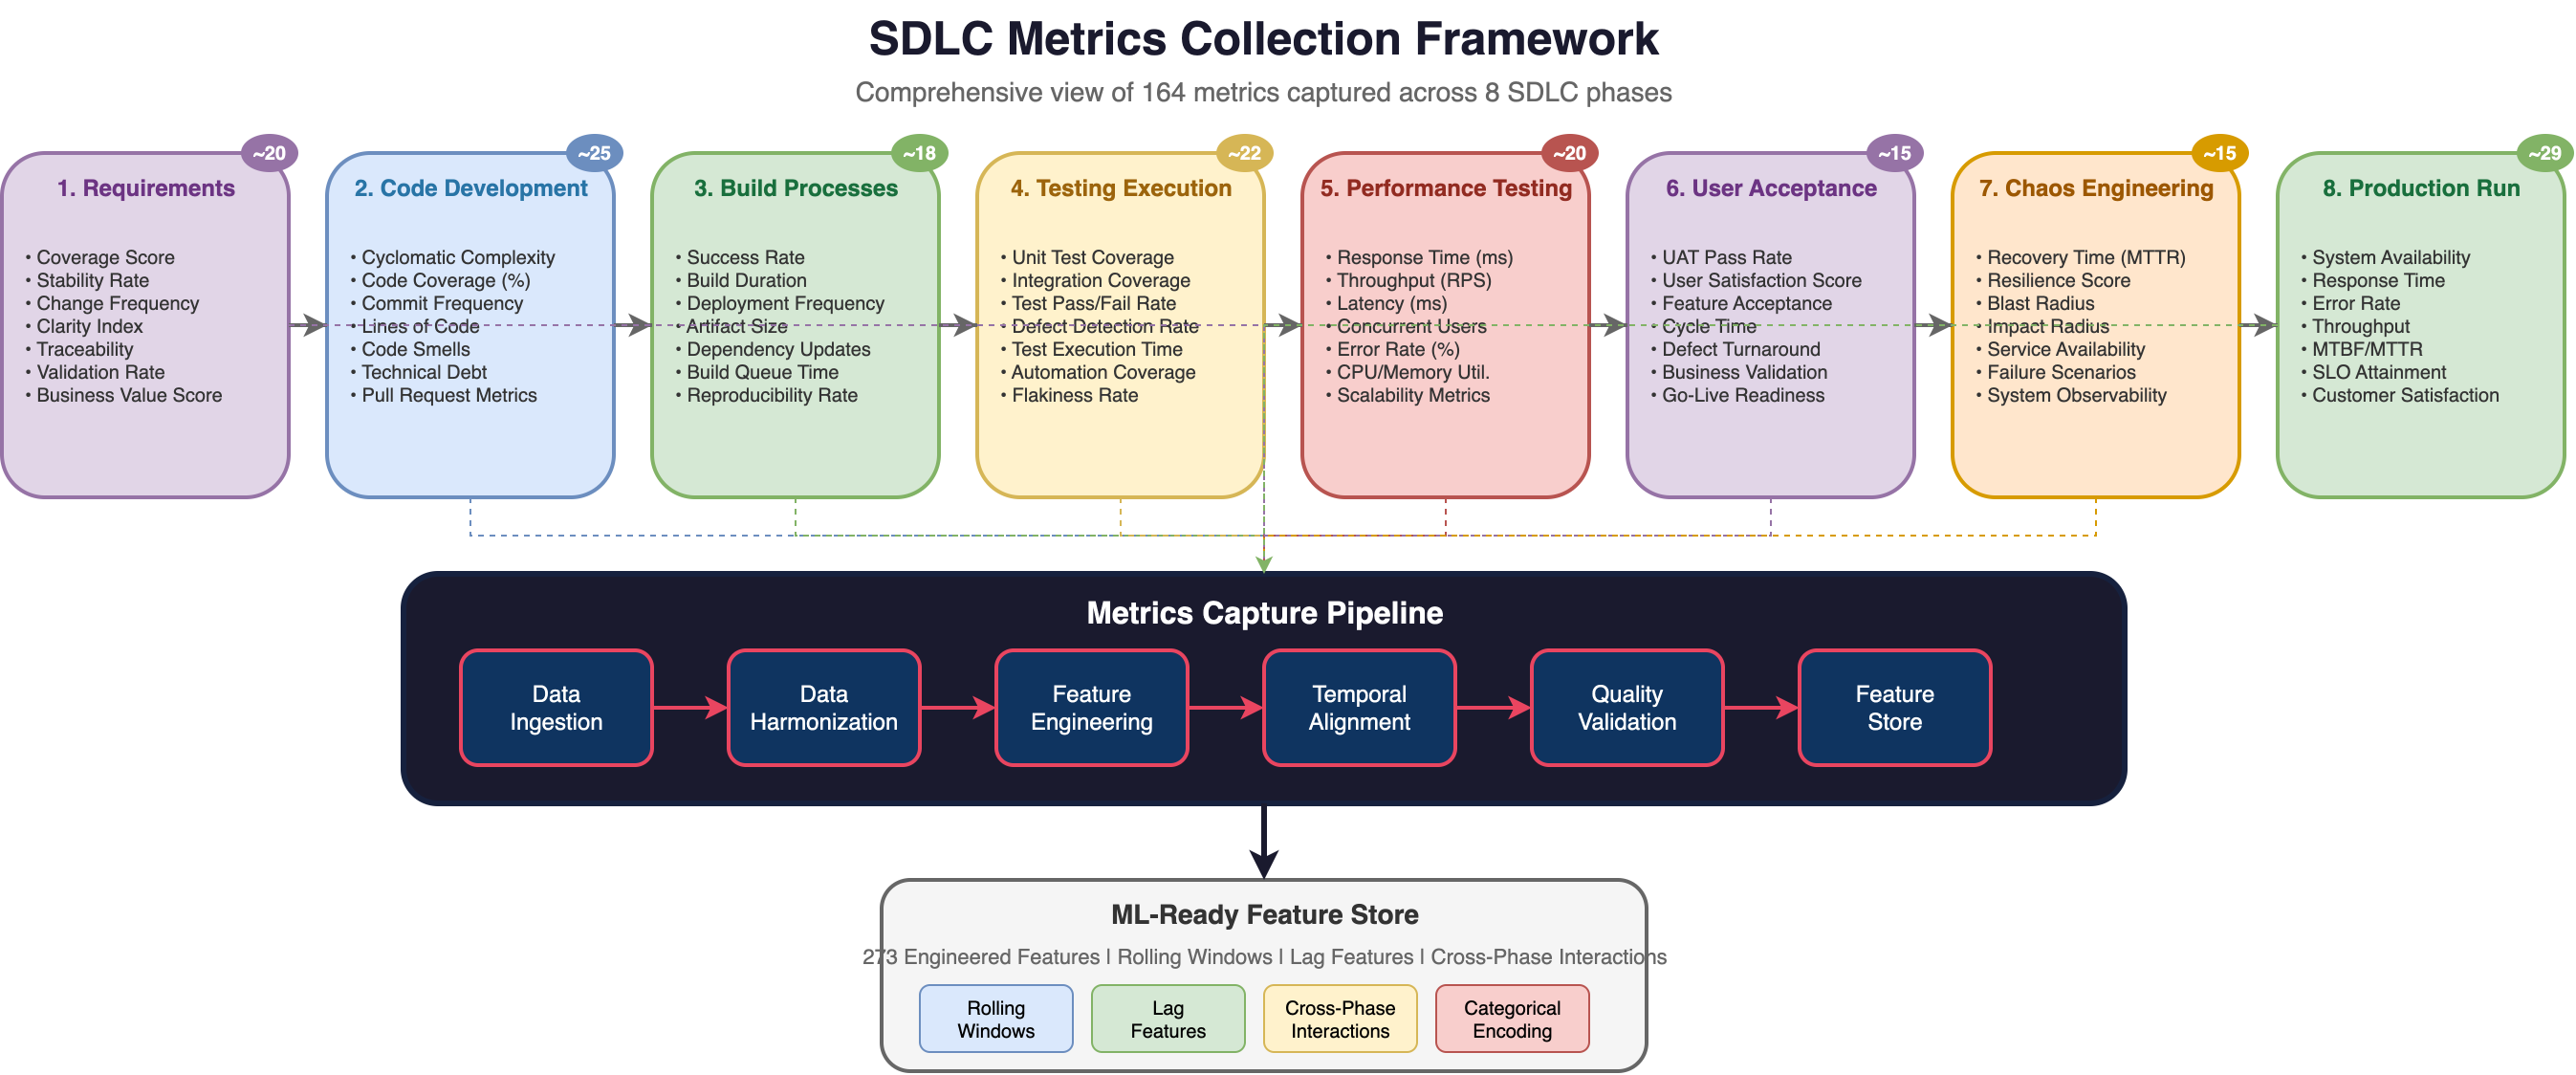
\includegraphics[width=\fulllength]{images/01-SDLC-Metrics-Collection-Framework.png}
\end{adjustwidth}
\caption{SDLC Metrics Collection Framework showing 164 metrics from
eight phases flowing through ingestion, processing, and storage layers
into 273 engineered features.\label{fig:sdlc_framework}}
\end{figure}

\subsubsection{Data Harmonization and
Standardization}\label{sec:harmonization}

Converting 164 distinct metrics across eight SDLC phases into consistent
machine learning features presents engineering complexity. Each metric
has unique characteristics:

\begin{itemize}
\item
  Cyclomatic complexity scores range from 1--50+ with logarithmic
  distributions
\item
  Code coverage percentages follow bounded normal distributions between
  0--100\%
\item
  Build success rates require binary encoding with temporal smoothing
\item
  Response times follow heavy-tailed distributions requiring statistical
  transformation
\end{itemize}

The pipeline implements intelligent data normalization strategies:

\textbf{Continuous Variable Normalization:}

\begin{equation}
x_{\text{normalized}} = \frac{\log(x + 1)}{\log(x_{\max} + 1)}
\end{equation}

for metrics with logarithmic distribution, and

\begin{equation}
x_{\text{normalized}} = \frac{x - \mu_x}{\sigma_x}
\end{equation}

for metrics with bounded distribution {[}0, 100{]}.

\textbf{Categorical Variable Encoding:}

\begin{itemize}
\item
  One-hot encoding for nominal categories (release type, environment)
\item
  Target encoding for high-cardinality categories (microservice ID)
\item
  Ordinal encoding for ranked categories (severity levels)
\end{itemize}

\subsubsection{Temporal Alignment and Feature
Engineering}\label{sec:temporal_alignment}

SDLC metrics have complex temporal relationships that must be preserved
during feature engineering. Code metrics measured at commit-level
granularity must align with build metrics captured per deployment cycle,
which in turn must synchronize with test metrics generated during
release validation.

\textbf{Temporal Alignment Strategy:}

\begin{enumerate}
\def\labelenumi{\arabic{enumi}.}
\item
  Define release as the primary temporal unit
\item
  Aggregate commit-level metrics to release level using statistical
  functions
\item
  Align performance outcomes to the corresponding release window
\item
  Handle missing values through forward-fill for time-series continuity
\end{enumerate}

Feature engineering transforms raw metrics into predictive signals
through:

\begin{itemize}
\item
  \textbf{Rolling window aggregations}: Moving averages, standard
  deviations, minima, maxima, and coefficients of variation across 3, 5,
  7, and 10 period windows
\item
  \textbf{Lag features}: Values from 1, 2, 3, and 5 previous releases to
  capture temporal dependencies
\item
  \textbf{Trend derivatives}: Rate of change calculations for
  identifying acceleration patterns
\item
  \textbf{Cross-phase features}: Interaction terms between metrics from
  different SDLC phases
\end{itemize}

\subsubsection{Synthetic Data Generation
Methodology}\label{sec:synthetic_data}

No public dataset combines SDLC process metrics with correlated runtime
system performance measurements. We confirmed this through an exhaustive
search of major ML data repositories (UCI Machine Learning Repository,
Kaggle, Zenodo, Papers with Code Datasets) and software engineering
benchmarks (TravisTorrent~\cite{beller2017travistorrent}, GHTorrent,
PROMISE repository). TravisTorrent captures CI/build metadata but lacks
runtime performance telemetry. Performance prediction
literature~\cite{ha2019, siegmund2015} operates on configuration
spaces, not development process metrics. The data required for
SDLC-to-performance correlation is inherently proprietary: it involves
internal build pipelines, deployment telemetry, test infrastructure
metrics, and production monitoring that organizations do not publicly
release due to competitive and security concerns. This absence of public
benchmarks is itself a contribution gap that our synthetic generator
addresses, providing the first reproducible dataset for this prediction
task.

To address this gap, we developed a reproducible synthetic data
generator that serves as both a validation instrument and a reusable
benchmark for future research. The generator employs a four-stage
pipeline:

\textbf{Stage 1: Marginal Distribution Specification.} We define 164
metrics across 8 SDLC phases (requirements, code, build, test,
performance testing, chaos testing, production, and UAT). Each metric is
assigned a parametric marginal distribution calibrated to published
industry benchmarks. Percentage metrics use Beta distributions with
domain-appropriate shape parameters; time-based metrics use log-normal
distributions; discrete counts use Poisson or negative binomial
distributions. Distribution parameters are calibrated against the DORA
2024 State of DevOps report~\cite{dora2024} and published enterprise
project statistics~\cite{forsgren2018}.

\textbf{Stage 2: Correlation Structure via Gaussian Copula.}
Inter-metric correlations are specified using domain expertise and
encoded into a \(164 \times 164\) correlation matrix. A Gaussian
copula~\cite{nelsen2006} generates correlated samples while preserving
each metric's marginal distribution:

\begin{enumerate}
\def\labelenumi{\arabic{enumi}.}
\item
  Sample
  \(\mathbf{Z} \sim \mathcal{N}(\mathbf{0}, \boldsymbol{\Sigma})\) using
  Cholesky decomposition
\item
  Transform to uniform: \(U_i = \Phi(Z_i)\)
\item
  Transform to target marginals: \(X_i = F_i^{-1}(U_i)\)
\end{enumerate}

where \(\boldsymbol{\Sigma}\) is the correlation matrix (ensured
positive semi-definite via Higham's alternating
projections~\cite{higham2002}), \(\Phi\) is the standard normal CDF,
and \(F_i^{-1}\) is the inverse CDF of each metric's specified
distribution. We specify 84 non-zero correlation pairs grounded in
domain knowledge (e.g., positive correlation between build success rate
and system uptime, negative correlation between change failure rate and
uptime).

Critically, the prediction target (System Uptime) is \emph{not} derived
from a deterministic function \(f(\mathbf{x})\). It is generated as a
copula-correlated metric with its own marginal distribution, meaning the
ML model must discover latent correlations rather than recover a known
function.

\textbf{Stage 3: Temporal Dynamics.} Raw copula samples are transformed
into realistic time series through:

\begin{itemize}
\item
  \textbf{AR(1) process}: Rank-preserving autoregression with lag-1
  correlation \(\rho = 0.55\)--\(0.65\) (domain-dependent), reflecting
  that consecutive releases share the same codebase and team context
\item
  \textbf{Maturity trend}: Gradual 3--8\% improvement over the
  observation window, reflecting organizational learning and tooling
  investment
\item
  \textbf{Release-type effects}: Quality metric modulation based on
  release type (Major releases show 3--8\% degradation; Patch releases
  show 2--5\% improvement)
\item
  \textbf{Shock events}: Stochastic ``bad release'' events
  (\(p = 0.03\)--\(0.05\)) with correlated multi-metric degradation and
  exponential recovery
\end{itemize}

\textbf{Stage 4: Statistical Validation.} Generated datasets are
validated against their specifications:

\begin{itemize}
\item
  Bounds compliance: all metric values within defined ranges (100\% pass
  rate)
\item
  Correlation preservation: 76--95\% of specified correlations realized
  within tolerance
  (\(|\rho_{\text{target}} - \rho_{\text{realized}}| < 0.5\), deliberately
  relaxed from \texttt{src/validator.py}'s general-purpose 0.15 default --
  see \texttt{generate.py}'s correlation-check step, which documents the
  rationale: the copula's positive-semi-definite correction and
  downstream temporal transforms attenuate specified correlations, so a
  stricter tolerance would fail checks for reasons unrelated to a
  specification error), with
  attenuation attributed to temporal dynamics
\item
  Completeness: zero missing values across all datasets
\end{itemize}

\textbf{Domain Profiles.} Three domain-specific configurations are
defined:

\begin{itemize}
\item
  \textbf{ABC Cloud Provider}: 170 releases over 5 years, 200+
  microservices, DORA ``High'' tier
\item
  \textbf{XYZ Sales Force}: 200 releases over 5.5 years, aggressive
  release cadence, DORA ``High'' tier
\item
  \textbf{Card Payment Processor}: 150 releases over 4 years
  ($\sim$one release every 9.7 days), PCI-DSS
  compliance, DORA ``High'' tier (relabeled from ``Elite'' -- Elite
  requires multiple deploys per day, which this cadence does not meet;
  High, defined as between once per week and once per month, is the
  correct tier for this release frequency)
\end{itemize}

\textbf{Reproducibility.} All generation parameters (distribution
specifications, correlation matrices, temporal dynamics, random seeds)
are published as YAML configuration files. The generator is
deterministic: identical seeds produce identical datasets. The complete
generator code and configuration will be released as a reusable
benchmark.

\textbf{Limitations of Synthetic Data:}

\begin{itemize}
\item
  Cannot capture emergent phenomena in real distributed systems
\item
  Copula-specified correlations may be simpler than real-world
  dependencies
\item
  Temporal dynamics are parametric approximations of complex
  organizational processes
\item
  Real-world validation with production SDLC data remains essential
  future work
\end{itemize}

\subsubsection{Data Quality and Anomaly
Detection}\label{sec:data_quality}

The pipeline implements range validation, statistical outlier detection
(z-score thresholds), cross-metric consistency checks, and missing value
handling (forward-fill for time series, mean imputation for
cross-sectional data). Quality scores influence model confidence
intervals in production deployment.

\subsection{Proposed Approach and Models}\label{sec:approach_models}

PRESTO employs a multi-layered architecture that transforms
heterogeneous SDLC metrics into performance forecasts through machine
learning techniques. Figure~\ref{fig:system_arch}
presents the complete system workflow, from SDLC metrics ingestion
through prediction generation, organized across five architectural
tiers.

\begin{figure}[H]
\begin{adjustwidth}{-\extralength}{0cm}
\centering
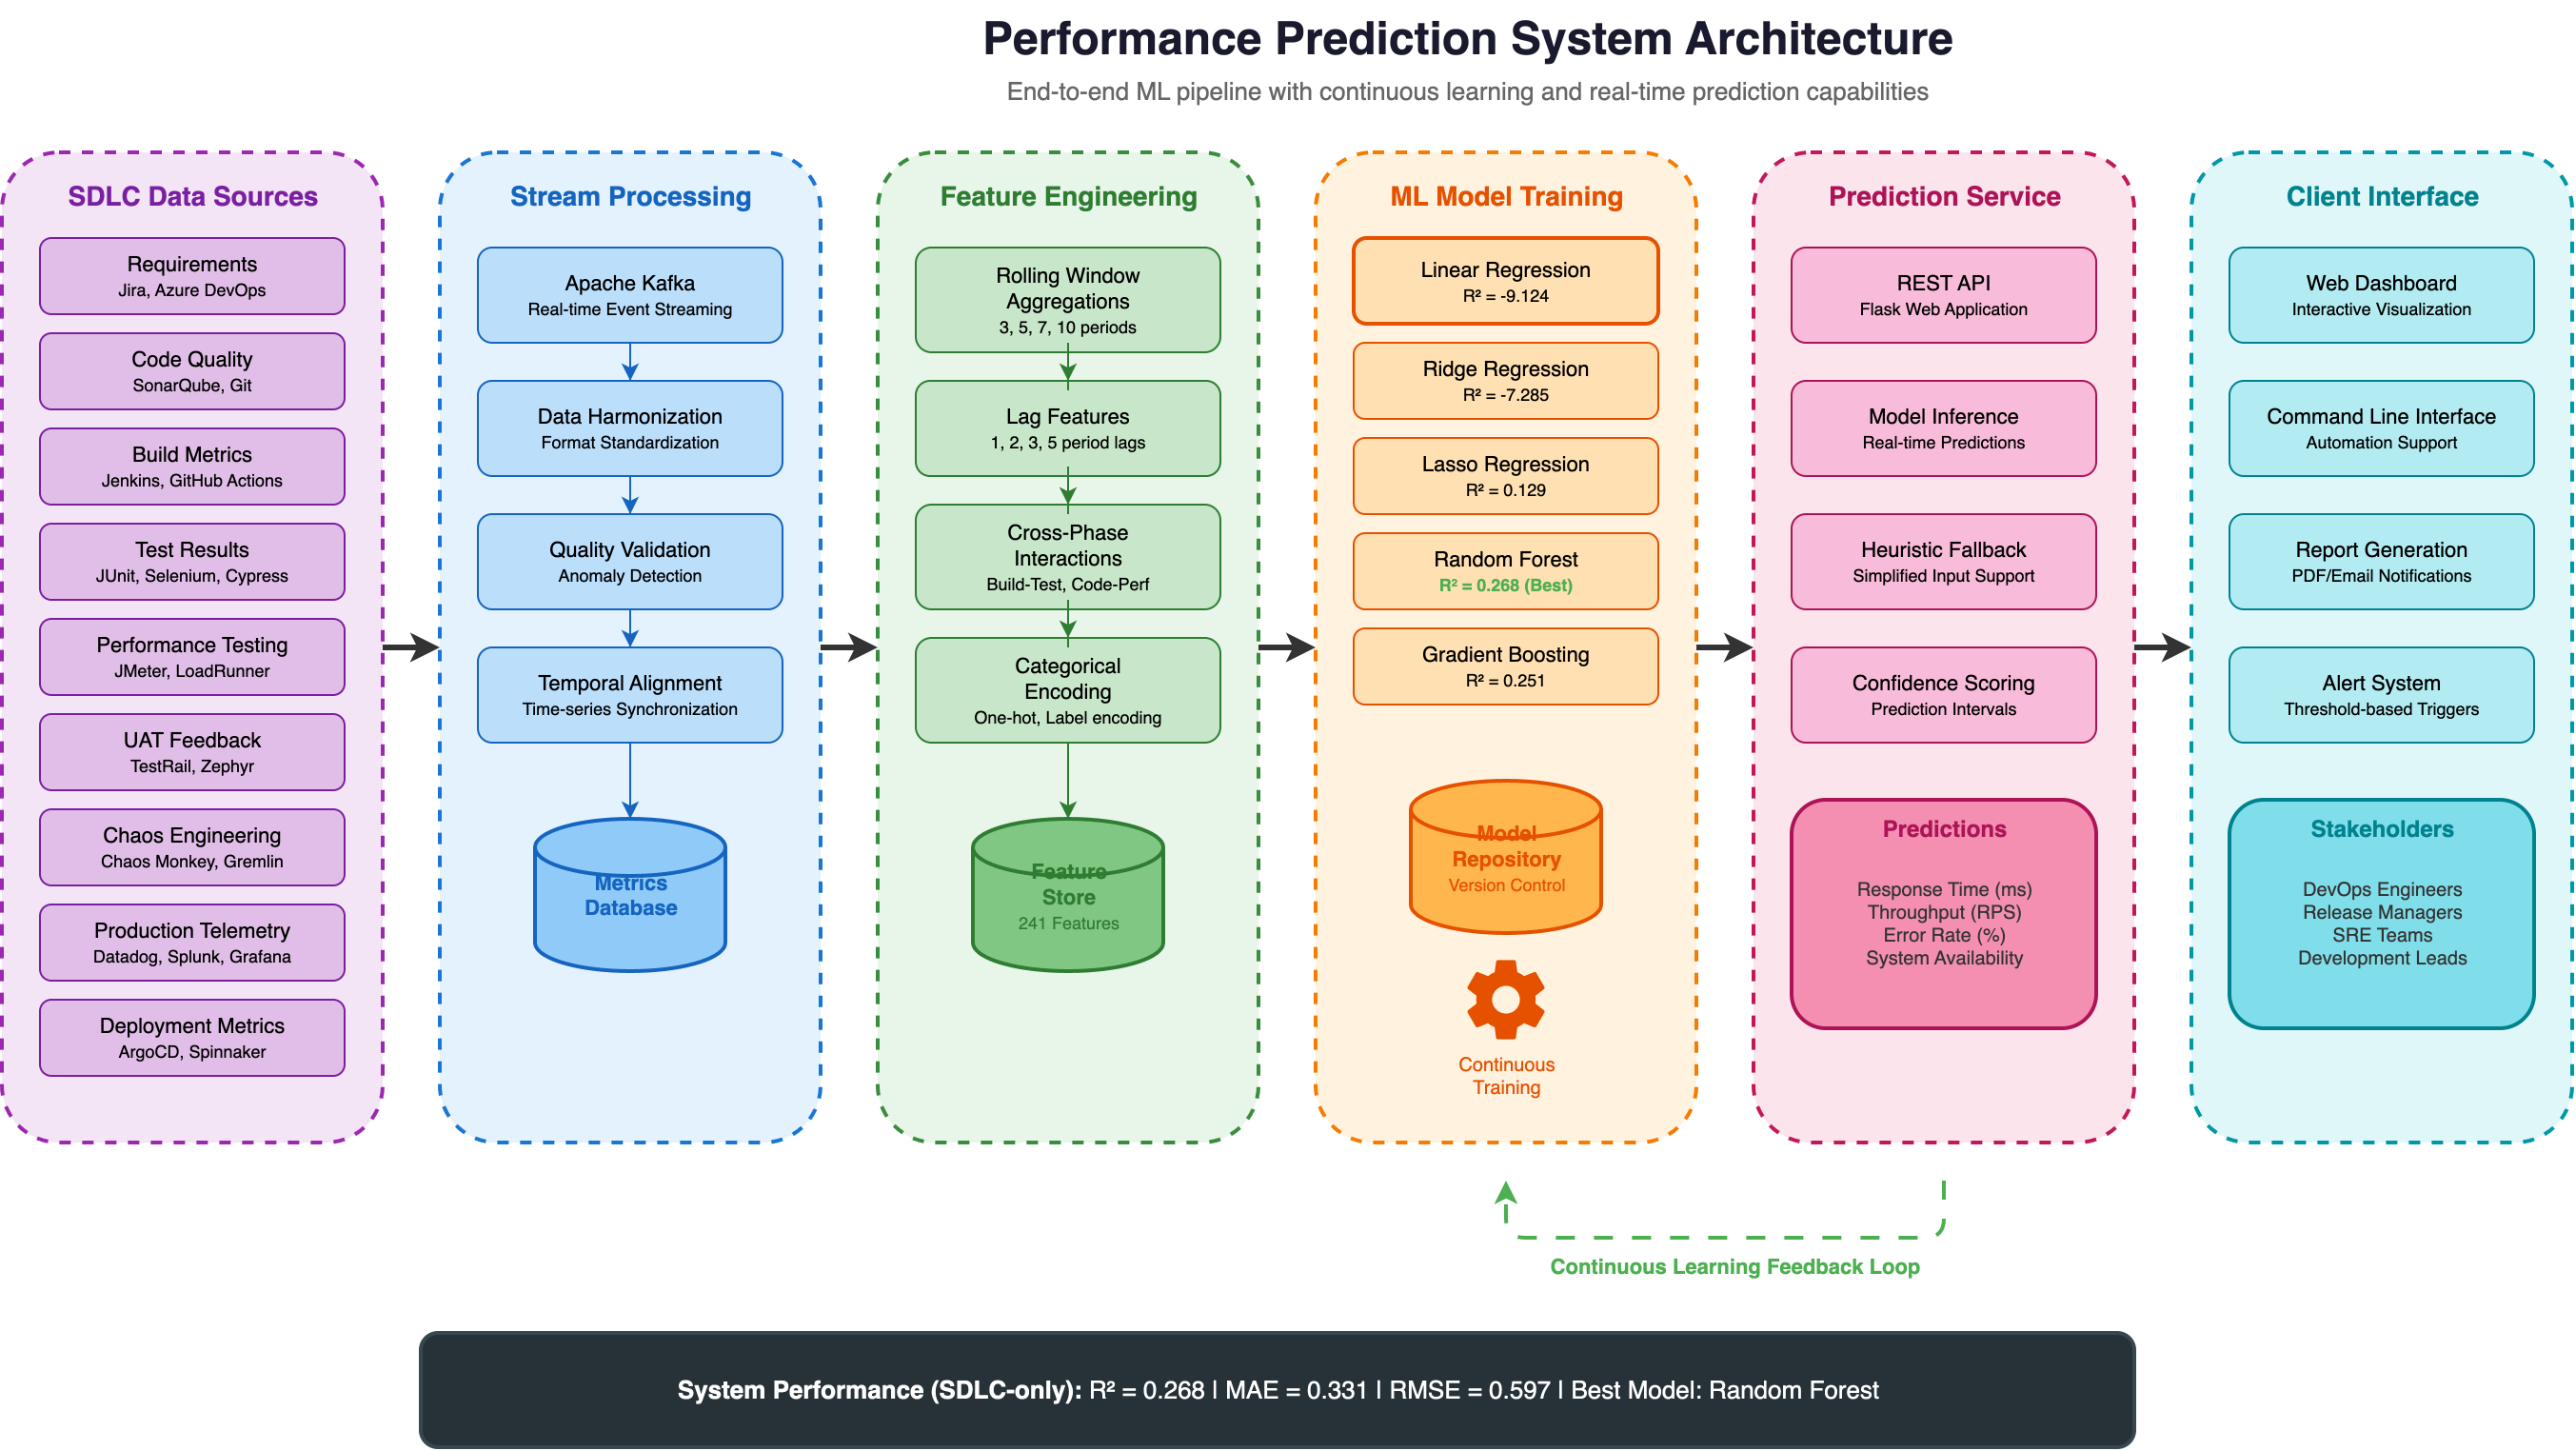
\includegraphics[width=\fulllength]{images/02-Performance-Prediction-System-Architecture.png}
\end{adjustwidth}
\caption{PRESTO System Architecture. Proposed end-to-end pipeline from
SDLC metric sources through feature engineering and ML model training to
prediction output.\label{fig:system_arch}}
\end{figure}

\subsubsection{Feature Engineering
Pipeline}\label{sec:feature_eng_pipeline}

\begin{figure}[H]
\begin{adjustwidth}{-\extralength}{0cm}
\centering
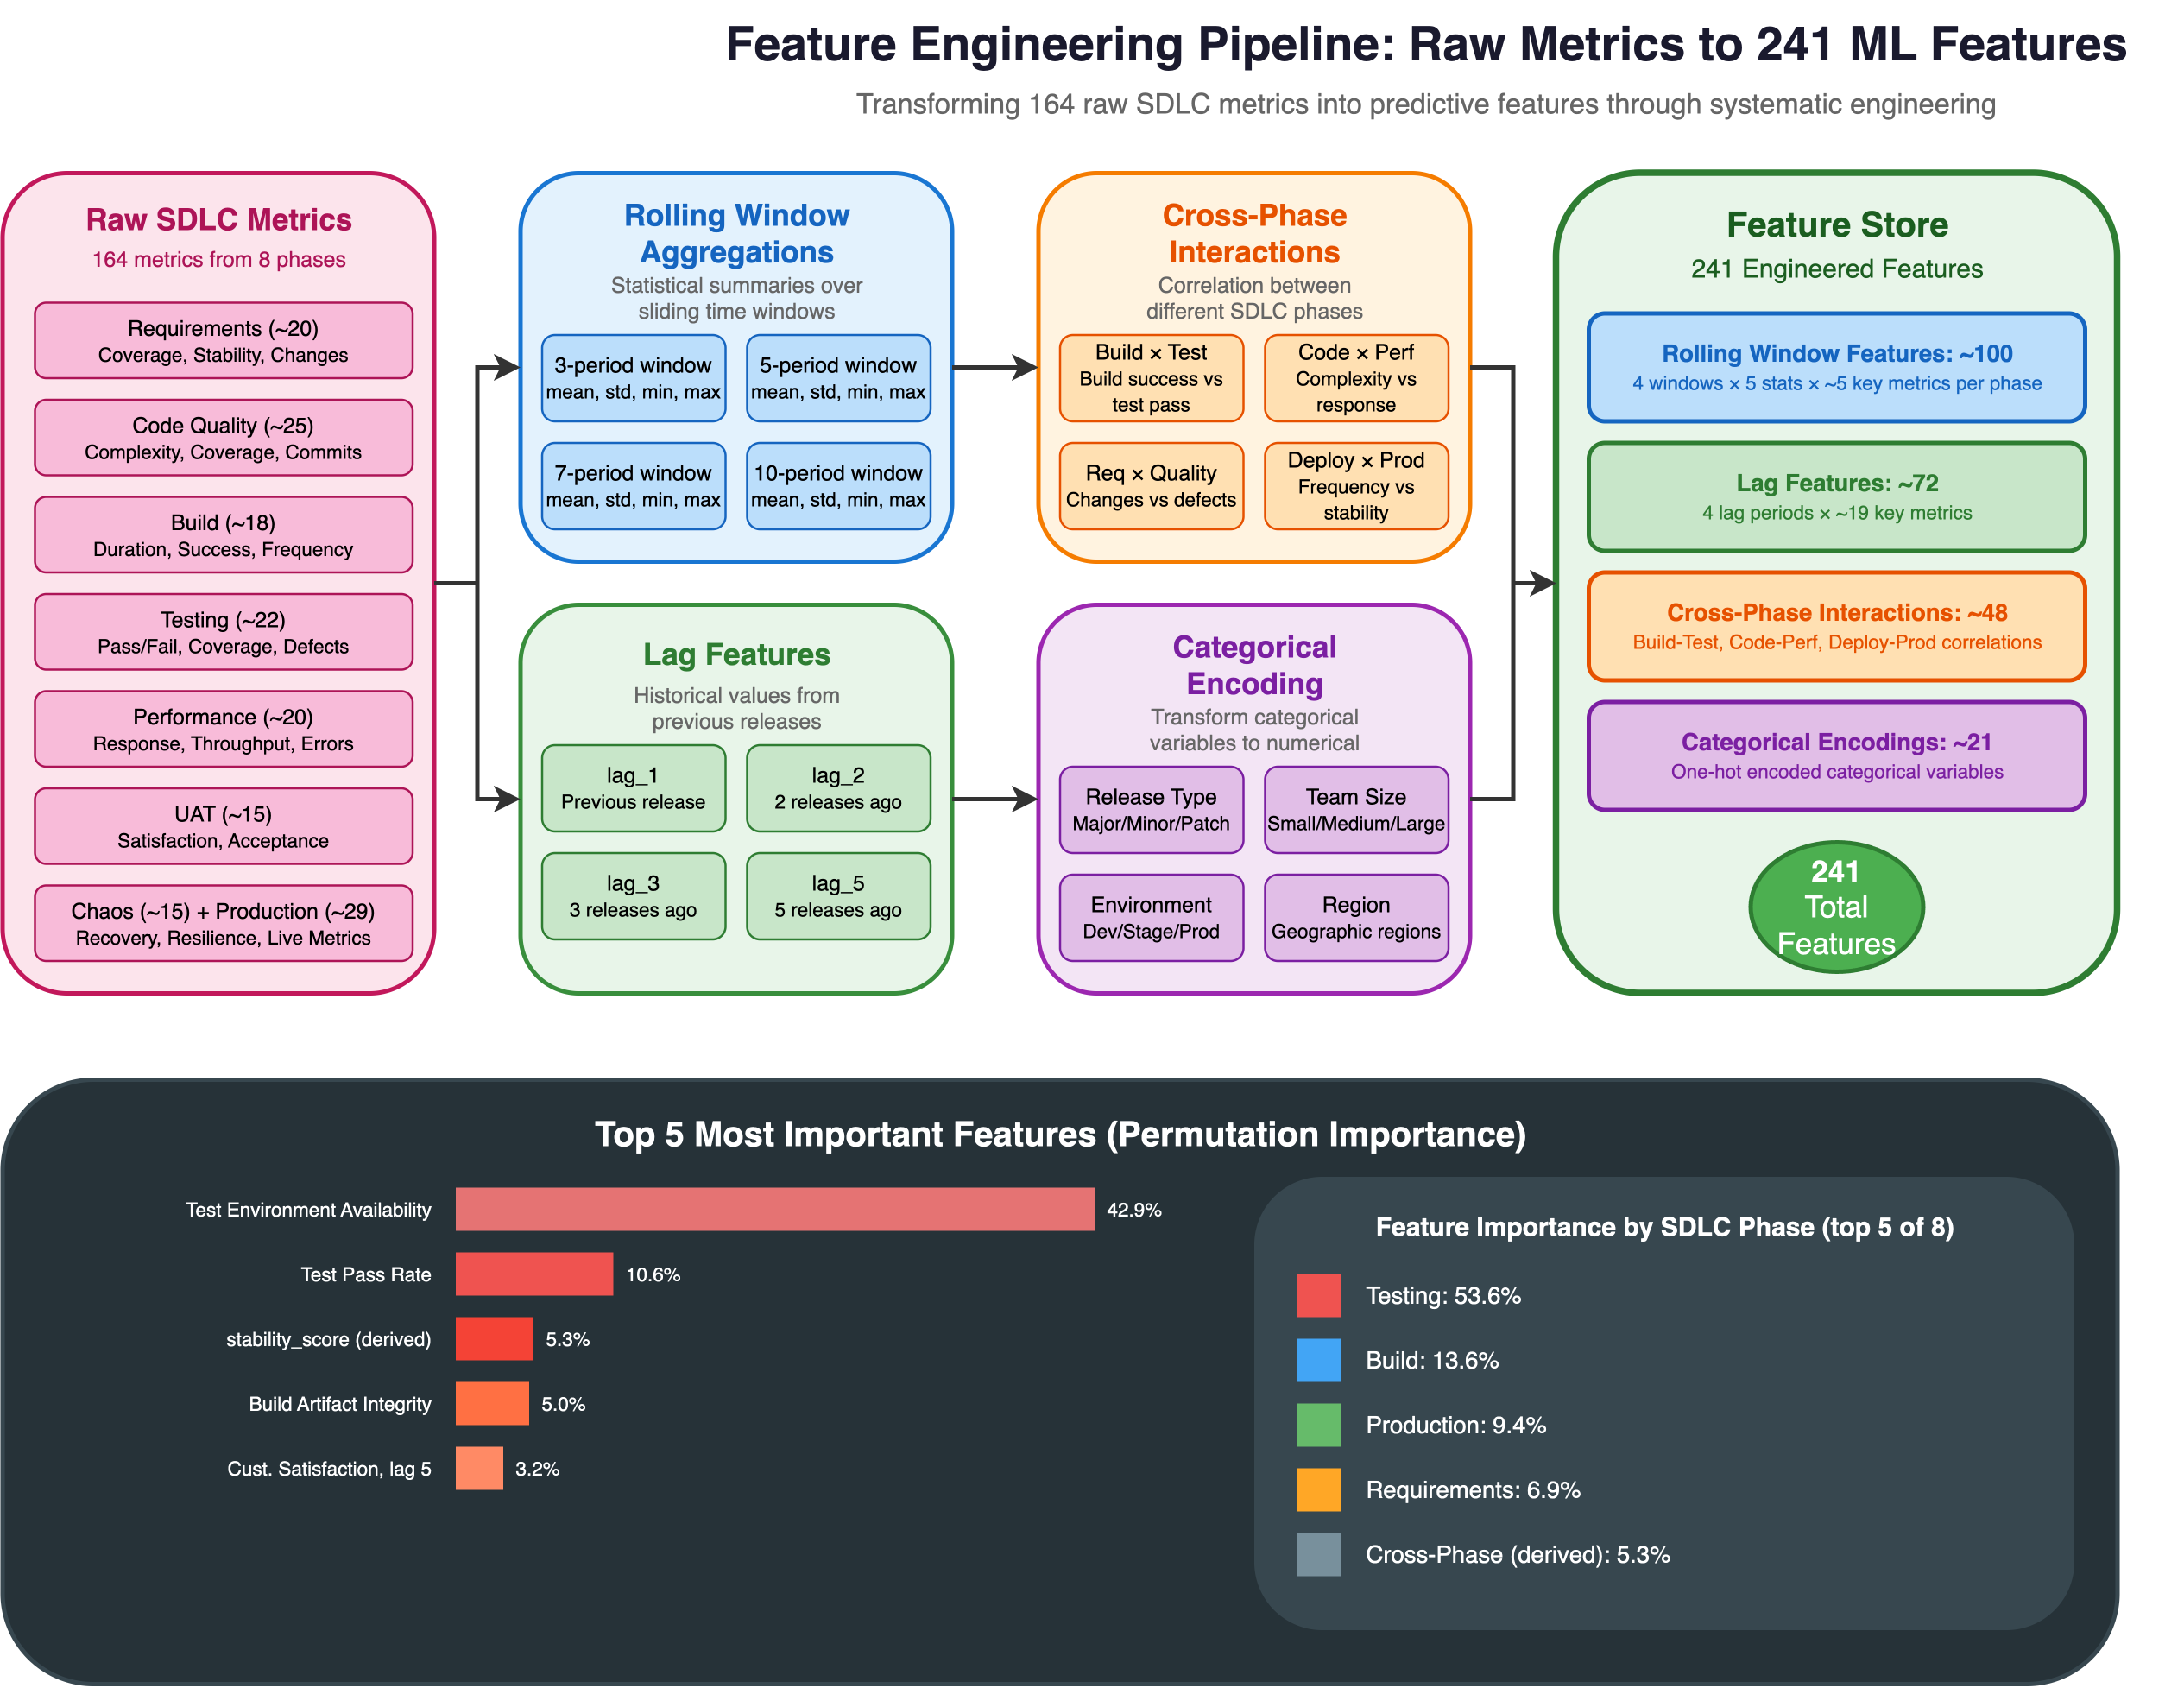
\includegraphics[width=\fulllength]{images/03-Feature-Engineering-Pipeline.png}
\end{adjustwidth}
\caption{PRESTO Feature Engineering Pipeline. Six-stage transformation
from raw SDLC metrics to a reduced feature set via PA-RFE (241 SDLC
features before reduction, 273 including autoregressive temporal
features).\label{fig:feature_pipeline}}
\end{figure}

Feature engineering represents the critical component for extracting
predictive signals from raw SDLC metrics.
Figure~\ref{fig:feature_pipeline} details the six-stage
transformation process from raw metrics through feature engineering and
phase-aware selection:

The pipeline generates candidate features in five stages, applies
variance-based filtering, then performs phase-aware dimensionality
reduction (Stage 6):

\textbf{Stage 1 -- Rolling Window Aggregations:} Four window sizes (3,
5, 7, 10 periods) with five statistics each (mean, standard deviation,
minimum, maximum, coefficient of variation) applied to key numeric
metrics. Window sizes correspond to sprint durations: 3 periods
(immediate history), 5 (one sprint cycle), 7 (weekly patterns), 10
(longer-term stability).

\textbf{Stage 2 -- Lag Features:} Values from 1, 2, 3, and 5 previous
releases for selected metrics, capturing immediate prior-release effects
(lag-1), short-term momentum (lag-2, lag-3), and release cycle patterns
(lag-5).

\textbf{Stage 3 -- Cross-Phase Interactions:} Multiplicative interaction
terms between metrics from different SDLC phases (e.g., build duration
\(\times\) code complexity, test coverage \(\times\) deployment
frequency).

\textbf{Stage 4 -- Categorical Encodings:} One-hot encoding of
categorical variables including release type (major, minor, patch),
environment tier, and domain-specific identifiers.

\textbf{Stage 5 -- Feature Selection:} From the initial candidate pool,
features with near-zero variance or high pairwise correlation
(\(r > 0.95\)) are removed. PRESTO retains \textbf{273 features}, of
which 241 are SDLC process features and 32 are autoregressive (AR)
temporal features (rolling windows and lags of System Uptime). The 32 AR
features are analyzed separately in Section~\ref{sec:leakage}.

\textbf{Stage 6 -- Phase-Aware Feature Selection (PA-RFE):} After AR
features are isolated, the remaining 241 SDLC features undergo
Phase-Aware Recursive Feature Elimination (PA-RFE), an algorithm
designed to reduce feature dimensionality while preserving cross-phase
coverage. Unlike standard RFE~\cite{guyon2002}, which eliminates
features globally by importance and can remove entire SDLC phases,
PA-RFE enforces a \emph{phase-balance constraint}: each of the eight
SDLC phases retains at least \(k_{\min}\) features throughout
elimination (we use \(k_{\min} = 2\)). This guarantees that the reduced
feature set maintains interpretable connections to all lifecycle phases,
which is central to PRESTO's cross-phase prediction thesis.

Algorithm~\ref{alg:parfe} presents the PA-RFE
procedure. To prevent selection bias from evaluating multiple feature
subsets on the same holdout data, we employ a three-way temporal split:
60\% training, 20\% validation, 20\% test. At each iteration, the
algorithm: (1)~trains a Gradient Boosting model on the training set;
(2)~computes permutation importance on the validation set
(\(n_{\text{repeats}} = 10\)), which is unbiased for correlated features
unlike impurity-based importance; (3)~eliminates up to \(s = 5\)
features with the lowest importance, \emph{skipping} any feature whose
removal would leave its SDLC phase below \(k_{\min}\). The algorithm
terminates when no features can be eliminated without violating the
constraint. The floor is \(k_{\min} \times 8 = 16\) for the eight SDLC
phases; the two cross-phase composites (\texttt{quality\_score},
\texttt{stability\_score}) form a virtual ninth group with
\(k_{\min} = 0\), allowing their free elimination. The optimal feature
subset corresponds to the iteration achieving maximum validation
\(R^2\), and final performance is reported on the truly held-out test
set (evaluated once).

\begin{algorithm}[H]
\caption{Phase-Aware Recursive Feature Elimination (PA-RFE)}\label{alg:parfe}
\begin{algorithmic}[1]
\Require Feature matrix $\mathbf{X} \in \mathbb{R}^{n \times p}$, target $\mathbf{y}$, phase map $\phi: \text{feature} \rightarrow \text{phase}$, min per phase $k_{\min}$, step size $s$
\Ensure Optimal feature subset $F^*$, ablation curve $\mathcal{C}$
\State $F \leftarrow \{f_1, \ldots, f_p\}$; $\mathcal{C} \leftarrow []$
\While{$|F| > k_{\min} \cdot |\text{phases}|$}
    \State Train model $M$ on $\mathbf{X}_{\text{train}}[F]$
    \State $\pi \leftarrow$ PermutationImportance($M$, $\mathbf{X}_{\text{val}}[F]$)
    \State Record $(|F|, R^2_{\text{val}})$ in $\mathcal{C}$
    \State Sort $F$ by $\pi$ ascending (least important first)
    \State $E \leftarrow \emptyset$ \Comment{elimination batch}
    \For{$f$ in sorted $F$}
        \If{$|E| \geq s$}
            \State \textbf{break}
        \EndIf
        \If{$|\{g \in F \setminus E : \phi(g) = \phi(f)\}| > k_{\min}$}
            \State $E \leftarrow E \cup \{f\}$
        \EndIf
    \EndFor
    \If{$E = \emptyset$}
        \State \textbf{break} \Comment{no features removable}
    \EndIf
    \State $F \leftarrow F \setminus E$
\EndWhile
\State $F^* \leftarrow \arg\max_{(|F|, R^2) \in \mathcal{C}} R^2$
\State \Return $F^*$, $\mathcal{C}$
\end{algorithmic}
\end{algorithm}

\begin{verbatim}
Algorithm: Phase-Aware Recursive Feature Elimination (PA-RFE)
Require: Feature matrix X in R^(n x p), target y,
         phase map phi: feature -> phase,
         min per phase k_min, step size s
Ensure:  Optimal feature subset F*, ablation curve C

F <- {f_1, ..., f_p}; C <- []
while |F| > k_min * |phases| do
    Train model M on X_train[F]
    pi <- PermutationImportance(M, X_val[F])
    Record (|F|, R^2_val) in C
    Sort F by pi ascending (least important first)
    E <- {}                                  // elimination batch
    for f in sorted F do
        if |E| >= s then
            break
        if |{g in F \ E : phi(g) = phi(f)}| > k_min then
            E <- E union {f}
    if E = {} then
        break                                 // no features removable
    F <- F \ E
F* <- argmax_{(|F|, R^2) in C} R^2
return F*, C
\end{verbatim}

\textbf{Algorithm (PA-RFE).} Phase-Aware Recursive Feature Elimination.

Each feature is mapped to its SDLC phase using the metric registry: base
metrics map directly, while derived features (rolling windows, lags,
percentage changes) inherit the phase of their parent metric. The
computational complexity is \(O(K \cdot n \cdot p \cdot r)\) where \(K\)
is iterations (\(\sim 45\)), \(n\) samples, \(p\) current features, and
\(r\) permutation repeats.

\subsubsection{Machine Learning Model
Architecture}\label{sec:ml_architecture}

The prediction system evaluates five regression algorithms selected to
span the complexity spectrum. Figure~\ref{fig:ml_comparison} compares their holdout $R^2$
(ABC Cloud Provider, without AR features) and contrasts each model's CV $R^2$ against its
holdout $R^2$, illustrating why this paper selects and reports by holdout score rather than
the noisier CV estimate (Section~\ref{sec:exp_setup_validation}).

\begin{figure}[H]
\begin{adjustwidth}{-\extralength}{0cm}
\centering
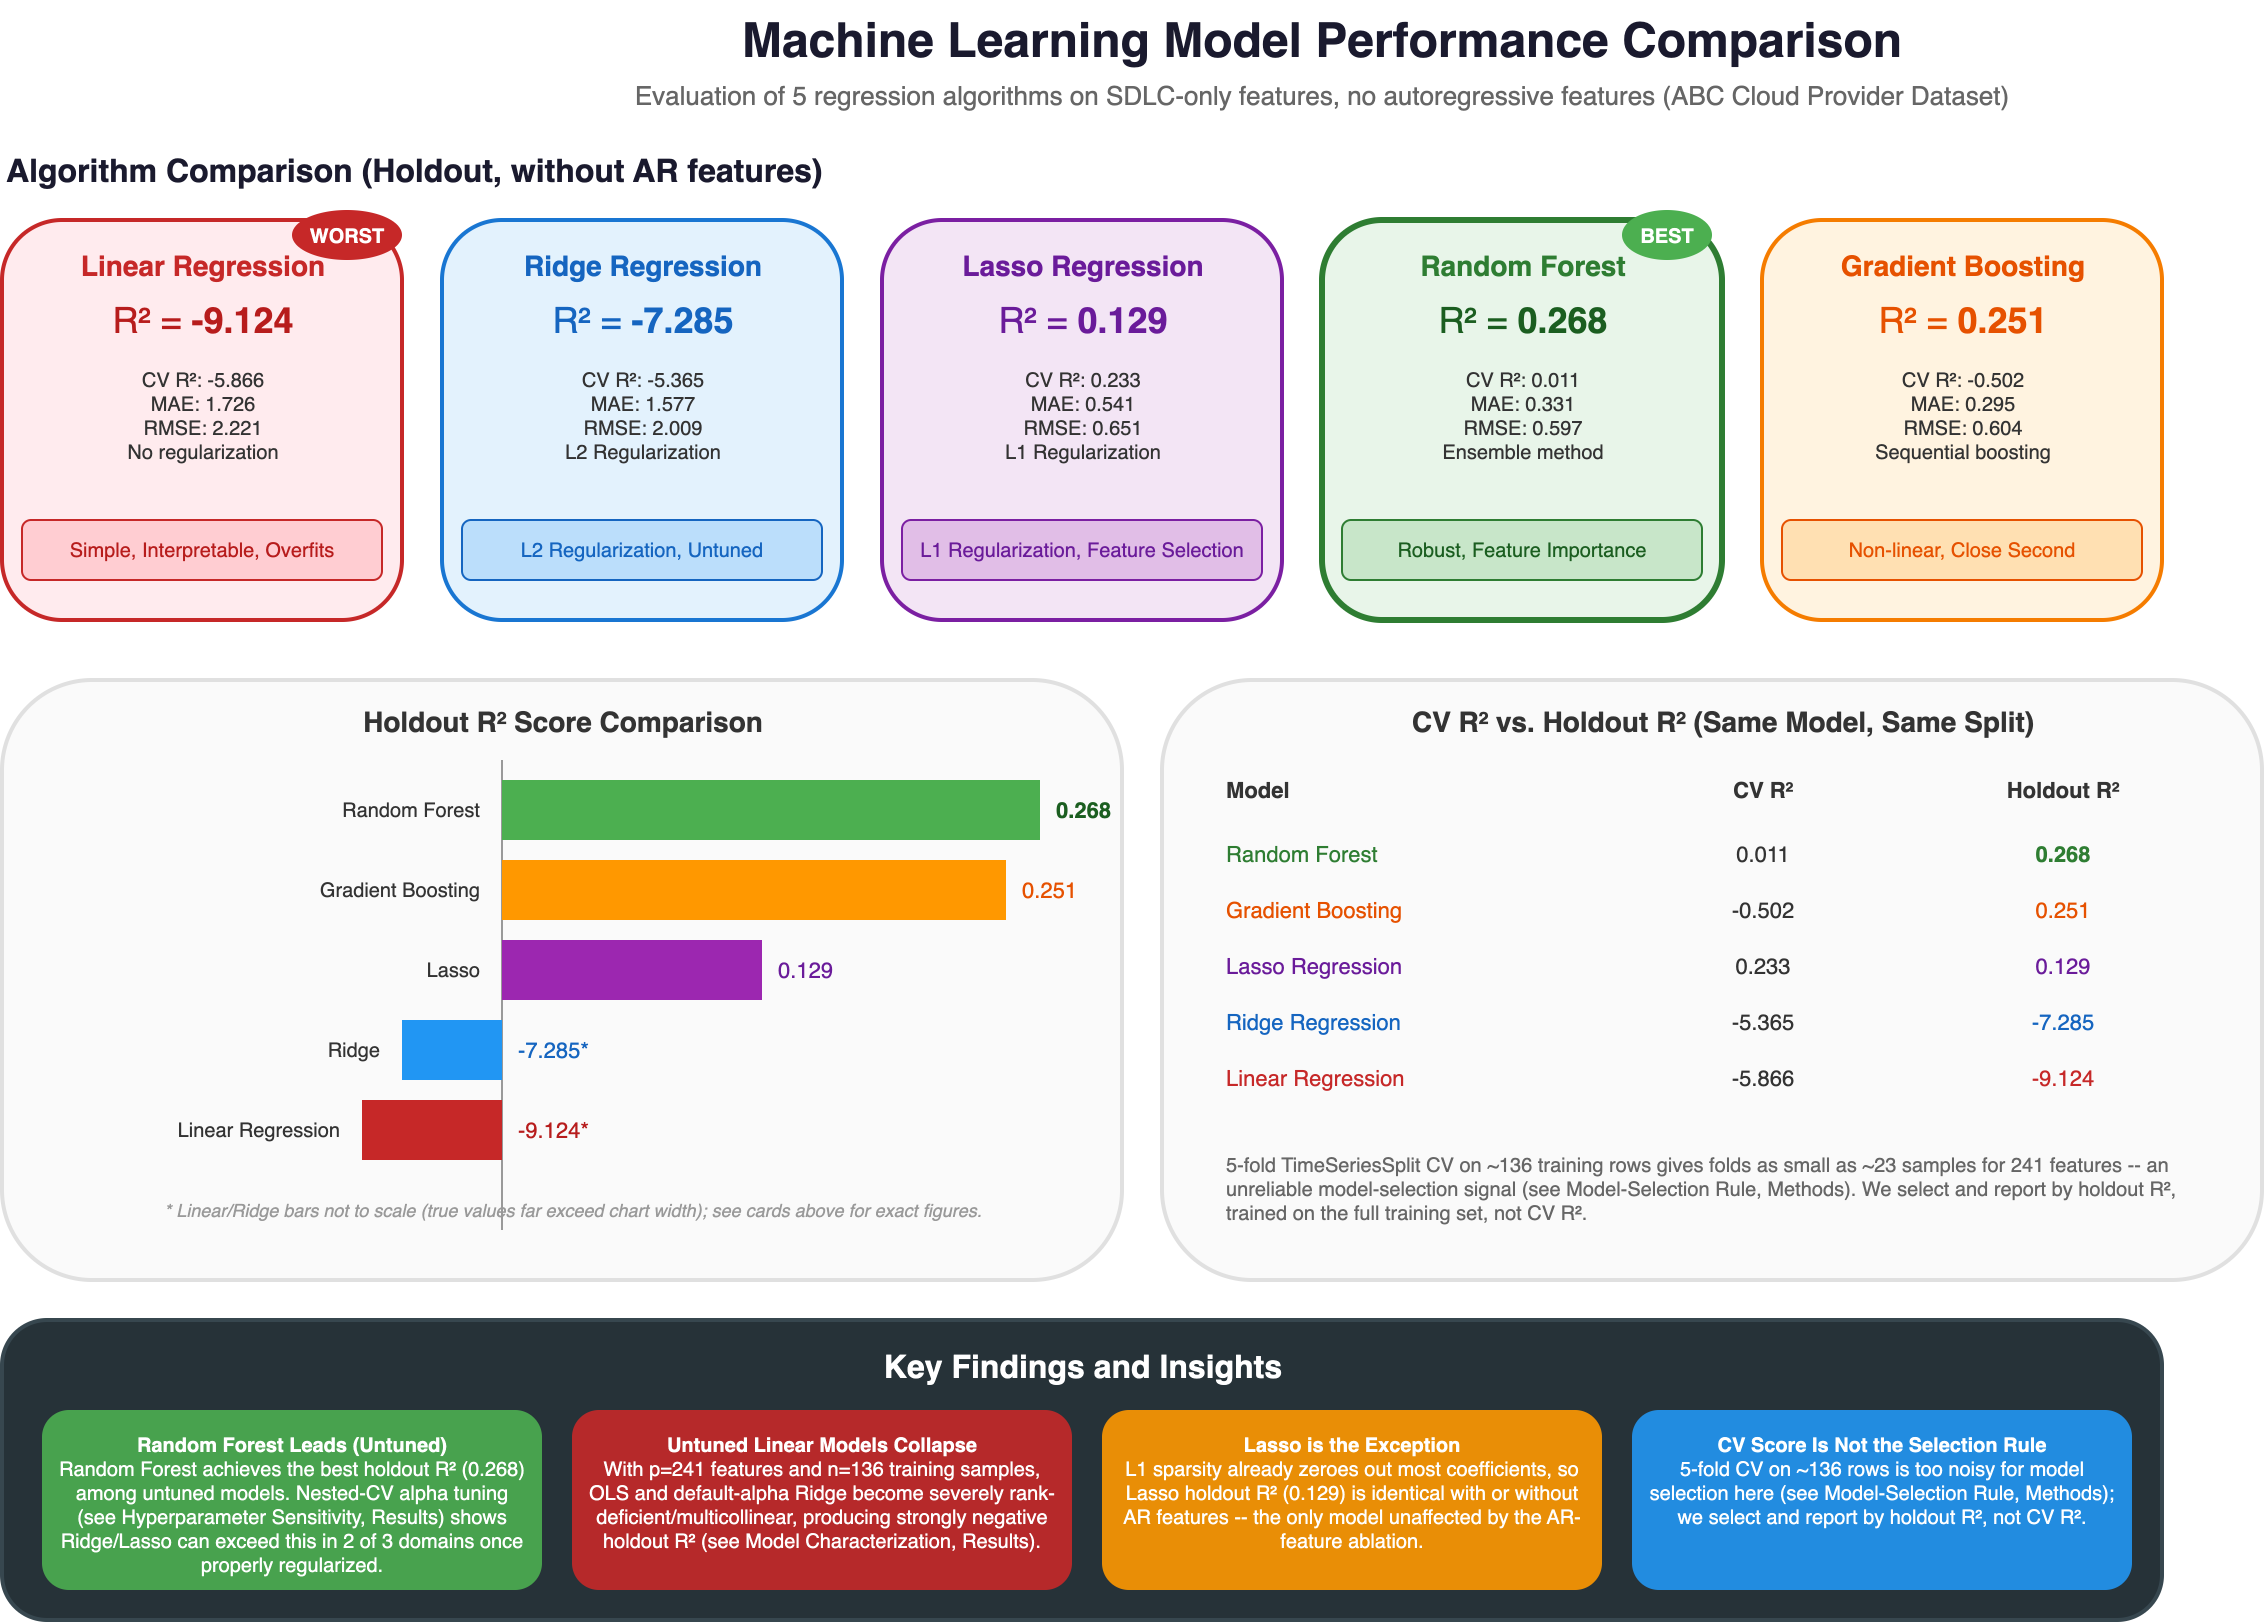
\includegraphics[width=\fulllength]{images/04-ML-Model-Comparison.png}
\end{adjustwidth}
\caption{Machine Learning Model Comparison. Holdout $R^2$ for all five models (ABC Cloud
Provider, without AR features), and CV $R^2$ vs. holdout $R^2$ per
model.\label{fig:ml_comparison}}
\end{figure}

\textbf{Algorithm Selection Rationale:}

\begin{enumerate}
\def\labelenumi{\arabic{enumi}.}
\item
  \textbf{Linear Regression (baseline)}: Provides interpretable
  baseline; success indicates feature engineering effectively linearizes
  relationships
\item
  \textbf{Ridge Regression}: Addresses multicollinearity through L2
  regularization; appropriate given correlated SDLC metrics
\item
  \textbf{Lasso Regression}: L1 regularization performs implicit feature
  selection; identifies dispensable features
\item
  \textbf{Random Forest}~\cite{breiman2001}: Bagged ensemble of
  decorrelated trees that handles high-dimensional correlated features
  through random subspace selection, relevant given our 241+ correlated
  SDLC metrics
\item
  \textbf{Gradient Boosting}~\cite{friedman2001}: Additive ensemble
  building sequential weak learners to correct residual errors, selected
  for its ability to capture cross-phase metric interactions without
  explicit interaction term specification
\end{enumerate}

\subsubsection{Hyperparameter Specifications}\label{sec:hyperparams}

{\def\LTcaptype{none} % do not increment counter
\begin{table}[H]
\centering
\caption{Hyperparameter configurations for all evaluated algorithms.\label{tab:hyperparams}}
\begin{tabular}{@{}llll@{}}
\toprule
\textbf{Algorithm} & \textbf{Parameter} & \textbf{Value} &
\textbf{Method} \\
\midrule
Ridge & alpha & 1.0 & Default \\
Lasso & alpha & 1.0 & Default \\
Random Forest & n\_estimators & 100 & Fixed \\
Random Forest & max\_depth & 10 & Fixed \\
Random Forest & min\_samples\_split & 5 & Fixed \\
Random Forest & min\_samples\_leaf & 2 & Fixed \\
Gradient Boost & n\_estimators & 100 & Fixed \\
Gradient Boost & max\_depth & 6 & Fixed \\
Gradient Boost & learning\_rate & 0.1 & Fixed \\
Gradient Boost & min\_samples\_split & 5 & Fixed \\
All models & random\_state & 42 & Fixed \\
All models & StandardScaler & fit on train only & -- \\
\bottomrule
\end{tabular}
\end{table}
}

Table~\ref{tab:hyperparams} reports the hyperparameter
configurations used for all results in
Sections~\ref{sec:model_perf}~through~\ref{sec:leakage} unless
otherwise noted. We deliberately used fixed hyperparameters
(scikit-learn defaults for regularization, community-standard values for
tree ensembles) without grid search, random search, or Bayesian
optimization, reasoning that with only 170 samples in the primary
dataset, hyperparameter tuning risks overfitting the validation folds.
We subsequently tested this reasoning directly: Section~\ref{sec:m3_tuning} reports a
nested-CV alpha-tuning pass for Ridge and Lasso specifically (a
leakage-safe design that never touches the holdout), and finds the
untuned alpha=1.0 default substantially understates linear-model
performance -- tuned linear models exceed Random Forest's holdout
\(R^2\) in 2 of 3 domains. The fixed-hyperparameter results elsewhere in
this paper are left as originally reported for consistency and because
they remain the paper's primary results, but readers should not infer
from them that linear models are inherently worse than tree ensembles on
this task.

\subsubsection{Experimental Setup and Validation
Strategy}\label{sec:exp_setup_validation}

\textbf{Dataset Characteristics:}

\begin{itemize}
\item
  \textbf{Primary dataset (ABC Cloud Provider)}: 170 releases, 5 years,
  200+ microservices
\item
  \textbf{Secondary dataset (XYZ Sales Force)}: 200 releases, 5.5 years,
  aggressive release cadence
\item
  \textbf{Tertiary dataset (Card Payment Processor)}: 150 releases, 4
  years, PCI-DSS compliance
\item
  \textbf{Feature space}: 273 engineered features (241 without AR
  features) from 8 SDLC phases
\item
  \textbf{Target variable}: System Uptime (\%)
\end{itemize}

\textbf{Validation Protocol:}

Because PRESTO forecasts performance from pre-deployment signals,
respecting chronological order is essential to avoid temporal data
leakage, a failure mode we characterized for build prediction in prior
work~\cite{mishra2026leakage}. We employed 5-fold expanding window
time-series cross-validation (sklearn
\texttt{TimeSeriesSplit(n\_\allowbreak splits=5)}) on the 80\% training partition to
respect temporal ordering. Each fold uses all prior data for training
and the next contiguous block for validation, ensuring models always
predict future releases from historical data only. Final holdout
evaluation uses the remaining 20\% (the most recent releases), never
seen during training or cross-validation.

\textbf{Model-Selection Rule.} Every algorithm comparison in this
paper -- which of 5 candidate models is ``best'' on the primary domain
(Section~\ref{sec:model_perf}), per synthetic domain (Section~\ref{sec:cross_domain}, Table
\ref{tab:cross_domain}), per TravisTorrent project (Section~\ref{sec:travistorrent}), and
which feature-selection method wins (Section~\ref{sec:parfe_results}, Table~\ref{tab:parfe_comparison}) -- selects by
\textbf{holdout \(R^2\), not mean CV \(R^2\)}, and we pre-declare this
rule explicitly here so it is stated once, before any results, rather
than left to be inferred separately four times. The alternative would
select differently: on the primary domain without AR features, mean CV
\(R^2\) favors Lasso (0.233) over Random Forest (0.011) -- the opposite
of the holdout-based ranking (Random Forest 0.268 vs.~Lasso 0.129)
reported as this paper's central RQ1 result throughout. We use holdout
\(R^2\) because 5-fold \texttt{TimeSeriesSplit} on a training partition
as small as 170 rows for 241 features produces early folds with as few
as \(\sim 23\) training samples (Section~\ref{sec:model_perf}'s CV-Holdout Discrepancy
note), an unreliable model-selection signal in this specific
small-\(n\), high-\(p\) regime; the holdout, trained on the full
training partition, is more representative of expected deployment
performance. This is a considered choice, not an unexamined default, and
we report CV \(R^2\) alongside holdout \(R^2\) throughout for
transparency rather than omitting it. \textbf{We are explicit that
pre-declaring this rule does not remove its bias, only discloses it}:
selecting the best of 5 candidate algorithms by their holdout score,
then reporting that same holdout score, carries a winner's-curse-style
optimism whether or not the selection procedure was announced in
advance. This optimism is smaller than what full hyperparameter tuning
would introduce, but it is not zero, and it compounds across the
roughly 100+ such selections made throughout this paper
(Section~\ref{sec:conclusion_validity} quantifies the resulting
comparison-family size and why we do not apply a formal
multiple-comparisons correction to it). The bootstrap confidence
intervals in Section~\ref{sec:bootstrap_ablation} quantify \emph{sampling}
variance in the already-selected model's holdout performance -- they do
not, and cannot, correct for the optimism introduced by the selection
step itself, since they resample the same holdout the model was chosen
on. We flag this distinction explicitly rather than let the CIs be read
as a stronger guarantee than they provide.

\textbf{Software Environment:}

\begin{itemize}
\item
  Python 3.14.5
\item
  scikit-learn 1.9.0
\item
  pandas 3.0.5
\item
  numpy 2.5.2
\item
  scipy 1.18.0
\end{itemize}

Pinned versions recorded in
\texttt{ENVIRONMENT.txt} (full path in the Data Availability Statement),
matching that same statement; this environment was
recreated fresh during the 2026-08-09 SSD migration and is not the
environment the original submission's numbers were computed under, which
was never separately recorded -- a previously identified reproducibility
gaps, now at least resolved going forward with a single,
consistently-cited environment record.

\begin{itemize}
\tightlist
\item
  Random seed: 42 (fixed for reproducibility)
\end{itemize}

\subsubsection{Continuous Learning and Model
Evolution}\label{sec:continuous_learning}

\begin{figure}[H]
\begin{adjustwidth}{-\extralength}{0cm}
\centering
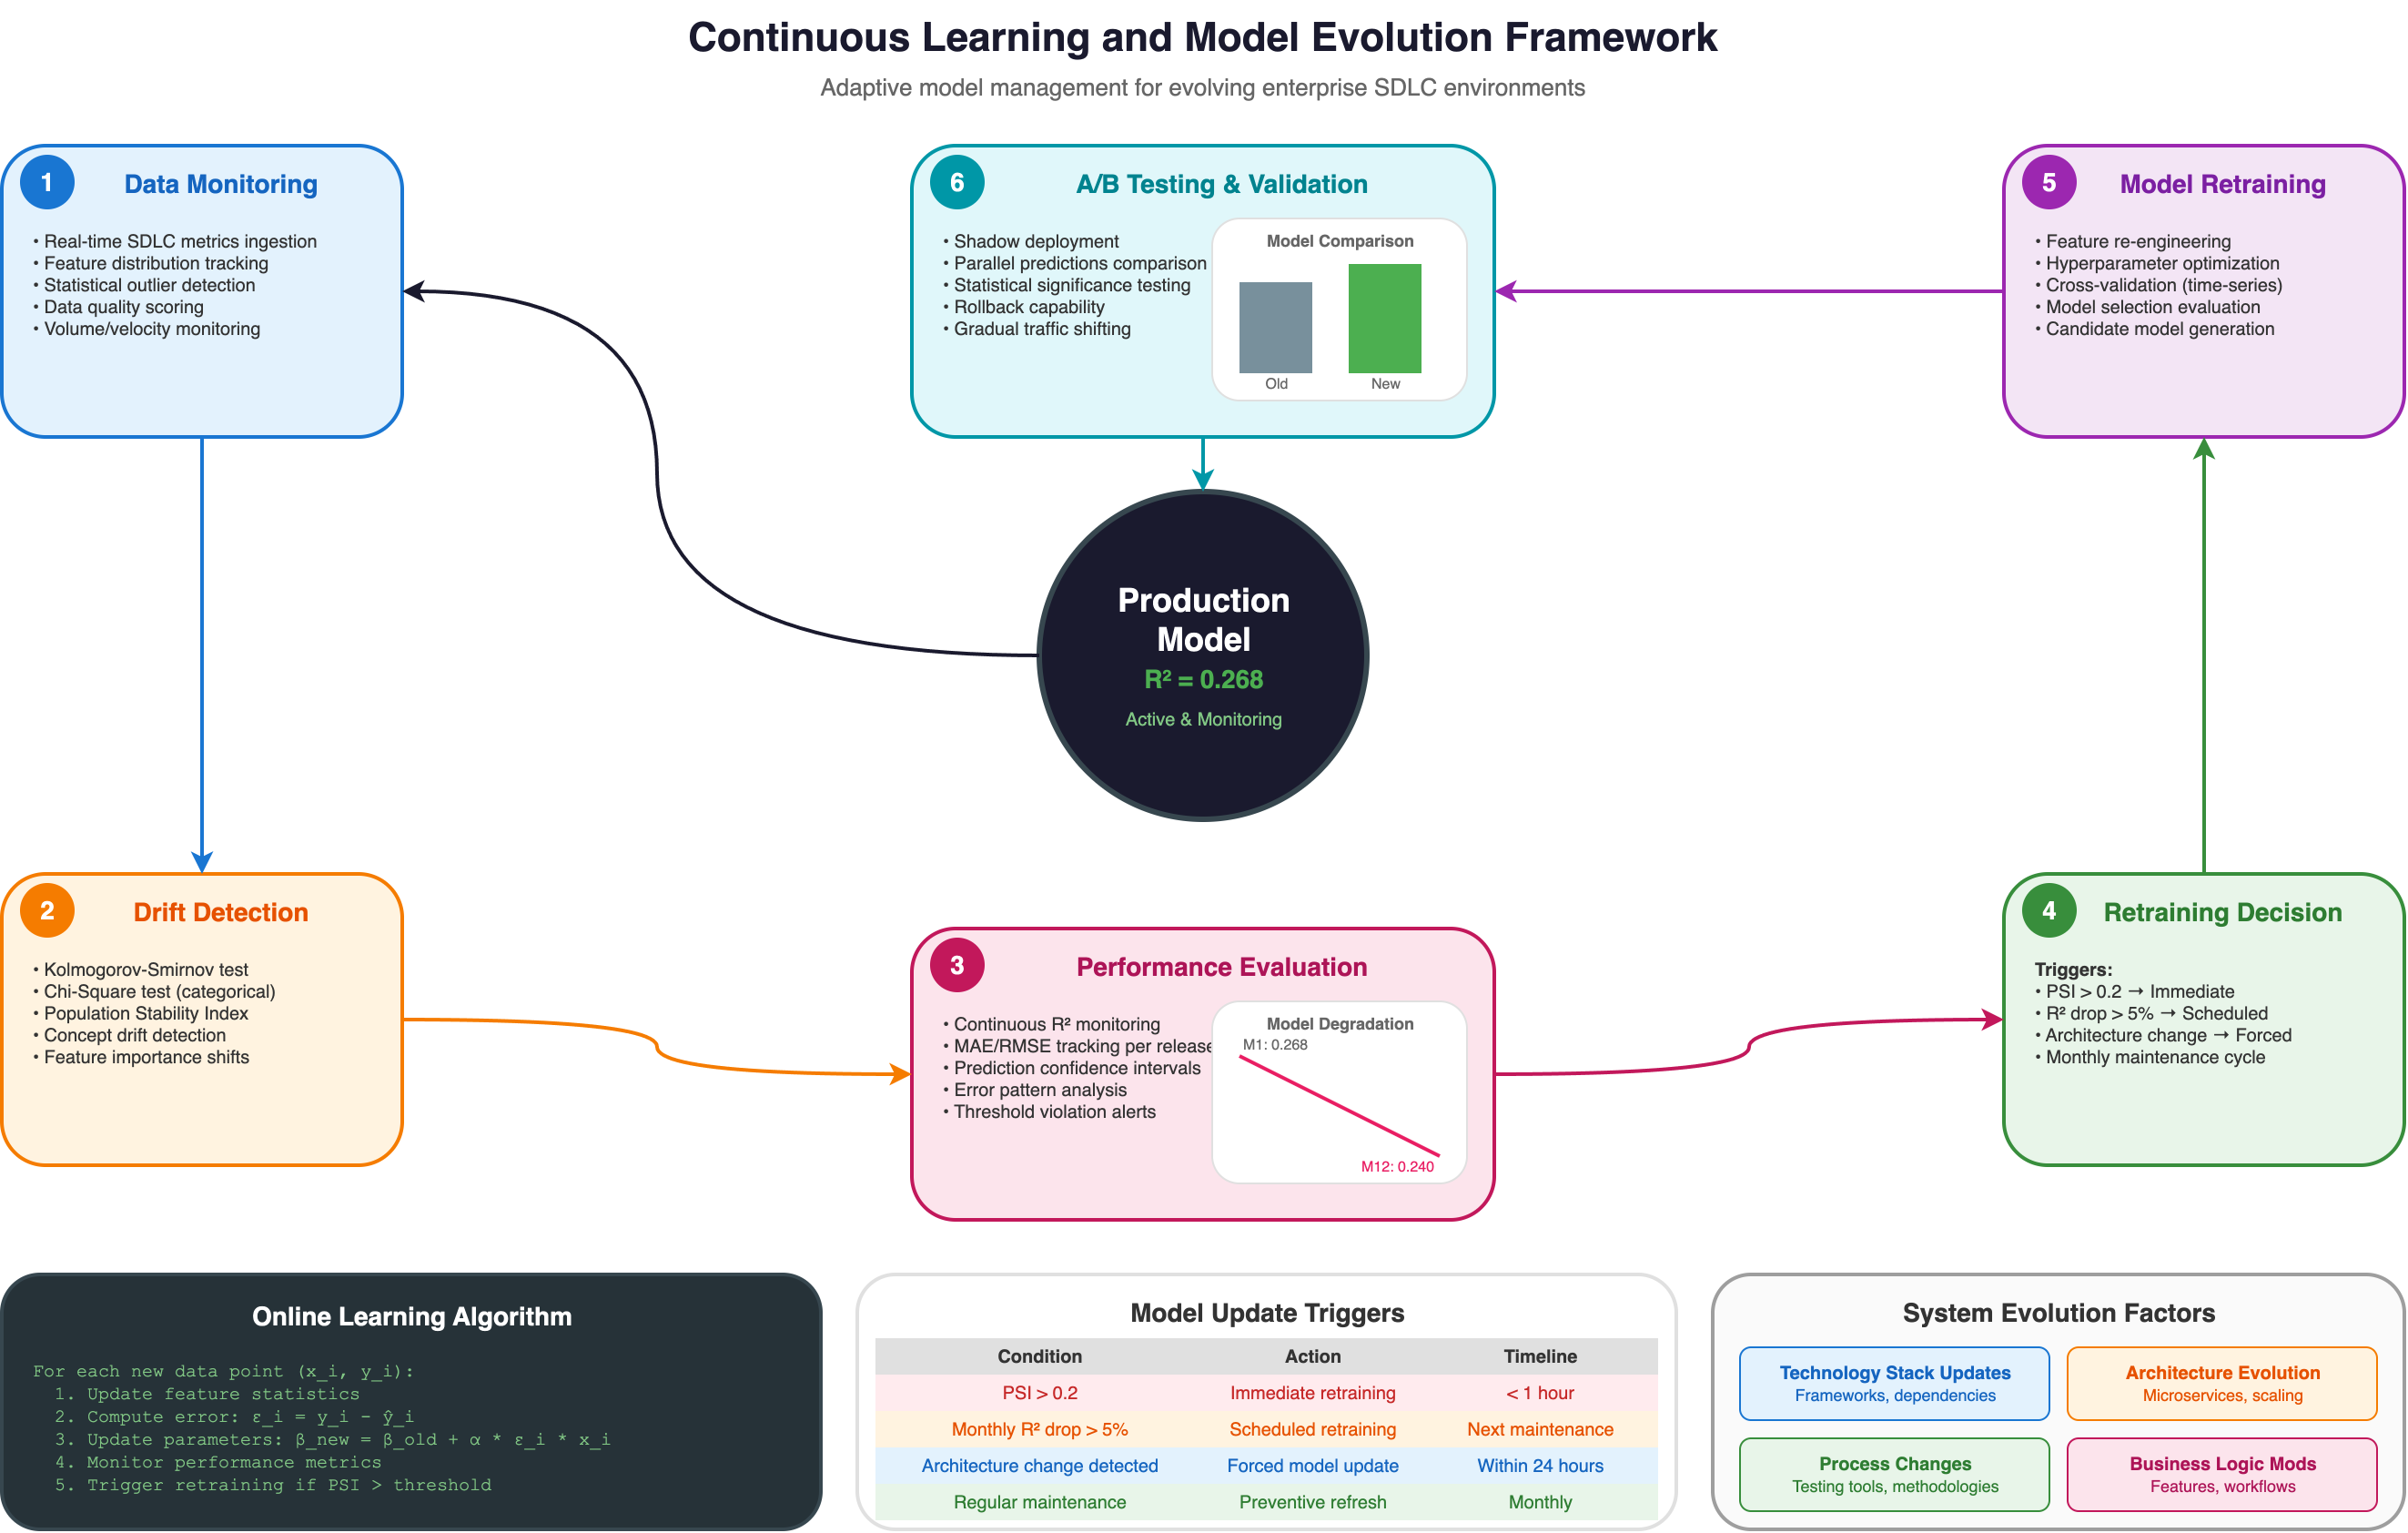
\includegraphics[width=\fulllength]{images/05-Continuous-Learning-Framework.png}
\end{adjustwidth}
\caption{Proposed Continuous Learning Framework (not experimentally
validated). Feedback loop from production prediction through drift
detection to automated retraining triggers.\label{fig:continuous_learning}}
\end{figure}

For production deployment, PRESTO's design includes a continuous
learning architecture to address concept drift~\cite{gama2014}.
Figure~\ref{fig:continuous_learning} illustrates the
proposed feedback loop (not experimentally validated in this study). The
framework monitors feature distribution shifts via Kolmogorov-Smirnov
tests, Chi-Square tests, and Population Stability Index (PSI),
triggering model retraining when PSI exceeds 0.2, monthly \(R^2\) drops
by more than 5\%, or a major architecture change is deployed.

\section{Results and Discussion}\label{sec:results}

This section presents experimental results from the PRESTO framework
implementation, analyzing model performance, feature importance, and
factors influencing prediction accuracy.

\subsection{Synthetic Domain Results}\label{sec:synthetic_results}

This subsection reports results on the three fully-synthetic,
copula-generated enterprise domains (ABC Cloud Provider, Card Payment
Processor, XYZ Sales Force). Section~\ref{sec:real_world_results} reports results on four
independent real-world datasets (TravisTorrent, Mozilla Perfherder,
GHALogs, SQuaD), kept in a separate subsection so synthetic and real
findings are never conflated.

\textbf{Note on regeneration (2026-08-09):} all synthetic-domain numbers
below were recomputed after fixing a same-row data-leakage bug in
\texttt{add\_rolling\_features()} (rolling-window statistics were
previously computed \emph{inclusive} of the current row instead of
shifted to strictly-prior releases -- see
\texttt{research-data/\allowbreak presto/\allowbreak code/\allowbreak synthetic\_\allowbreak data\_\allowbreak generator/\allowbreak R2\_\allowbreak LAG\_\allowbreak SHIFT\_\allowbreak FIX\_\allowbreak EVIDENCE.md}
for the full bug report and a controlled before/after comparison). The
regeneration also ran under a different, newly-pinned
numpy/scipy/scikit-learn environment than originally produced the
submitted numbers (see the same file's Addendum 2), which independently
shifts some figures -- the exact original environment was never
recorded, which is itself a previously identified reproducibility gap. Both
the generator code and this regenerated data, together with the pinned
environment, are deposited at \texttt{research-data/presto/} (to be
published as the camera-ready reproducibility package).

\subsubsection{Experimental Setup}\label{sec:results_setup}

We report results on the ABC Cloud Provider (170 releases, primary
dataset) unless otherwise stated; cross-domain results appear in Section~\ref{sec:cross_domain}. Dataset characteristics and validation protocol are detailed in
Section~\ref{sec:exp_setup_validation}. Of the 273 engineered features, 32 are derived from the
target variable itself (System Uptime rolling windows and lags). Of
these 32, 20 (rolling mean/std/min/max/cv across four windows) are
genuinely \textbf{autoregressive (AR) features} after the shift fix --
legitimate use of prior-period history, not leakage -- and 12
(lag/diff/pct-change) were already correctly shifted. We report all
results both \emph{with} and \emph{without} these 32 AR features to
transparently separate SDLC predictive signal from autocorrelation.
Following the corrected-pipeline evidence, we retire the term ``target
leakage'' for this feature set (the bug that justified it is fixed) in
favor of ``AR features'' throughout, reserving ``leakage'' for the
historical bug description.

\subsubsection{Model Performance Comparison (RQ1 and
RQ3)}\label{sec:model_perf}

\textbf{Answer to RQ1:} SDLC process metrics achieve R\(^2\) =
0.25--0.36 across three enterprise domains, beating all naive baselines
but falling far short of the R\(^2\) = 0.79--0.97 achievable when
historical performance (AR) features are included. These point estimates
are real, but bootstrap 95\% CIs are wide and, for most individual
domains, include zero (see ``Bootstrap Confidence Intervals and
Target-Correlation Ablation'' below); a target-correlation ablation
further shows that on synthetic data this signal is recovery of the
copula's hand-specified structure rather than independent discovery --
the Real-World Validation results later in this section, not the
synthetic domains alone, are what should be read as evidence of genuine,
transferable signal.

\textbf{Answer to RQ3:} With the untuned default hyperparameters used
throughout this paper (alpha=1.0), Random Forest achieves the best or
near-best holdout R\(^2\) on SDLC-only features in 2 of 3 domains, and
Linear/Ridge models collapse to strongly negative R\(^2\) due to
multicollinearity in the 241-feature space. However, nested-CV alpha
tuning (Section~\ref{sec:m3_tuning}) shows this collapse is substantially a
hyperparameter artifact, not an inherent property of linear models: once
tuned, Ridge or Lasso actually \emph{exceeds} Random Forest's holdout
R\(^2\) in 2 of the 3 domains (Card Payment, XYZ Sales). Random Forest
remains best only on the primary domain (ABC Cloud Provider) after
tuning. ``Trees are necessary'' should therefore be read as a
primary-domain, untuned-baseline finding, not a general one.

We evaluated five regression algorithms under two experimental
conditions: (a) with all 273 engineered features including the 32 AR
features, and (b) with 241 features after removing them. Table
\ref{tab:model_perf_with} and Table~\ref{tab:model_perf_without}
present the results for the ABC Cloud Provider dataset.

{\def\LTcaptype{none} % do not increment counter
\begin{table}[H]
\centering
\caption{Model performance comparison with AR features (ABC Cloud Provider).\label{tab:model_perf_with}}
\begin{tabular}{@{}lllll@{}}
\toprule
\textbf{Model} & \textbf{CV \(R^2\)} & \textbf{Holdout \(R^2\)} &
\textbf{MAE} & \textbf{RMSE} \\
\midrule
\textbf{Random Forest} & \textbf{0.690} & \textbf{0.950} &
\textbf{0.071} & \textbf{0.156} \\
Gradient Boosting & 0.211 & 0.865 & 0.120 & 0.256 \\
Lasso Regression & 0.233 & 0.129 & 0.541 & 0.651 \\
Ridge Regression & \(-0.815\) & \(-0.194\) & 0.589 & 0.762 \\
Linear Regression & \(-0.876\) & \(-0.256\) & 0.610 & 0.782 \\
\bottomrule
\end{tabular}
\end{table}
}

{\def\LTcaptype{none} % do not increment counter
\begin{table}[H]
\centering
\caption{Model performance comparison without AR features (ABC Cloud Provider).\label{tab:model_perf_without}}
\begin{tabular}{@{}lllll@{}}
\toprule
\textbf{Model} & \textbf{CV \(R^2\)} & \textbf{Holdout \(R^2\)} &
\textbf{MAE} & \textbf{RMSE} \\
\midrule
\textbf{Random Forest} & 0.011 & \textbf{0.268} & \textbf{0.331} &
\textbf{0.597} \\
Gradient Boosting & \(-0.502\) & 0.251 & 0.295 & 0.604 \\
Lasso Regression & 0.233 & 0.129 & 0.541 & 0.651 \\
Ridge Regression & \(-5.365\) & \(-7.285\) & 1.577 & 2.009 \\
Linear Regression & \(-5.866\) & \(-9.124\) & 1.726 & 2.221 \\
\bottomrule
\end{tabular}
\end{table}
}

\begin{figure}
\centering
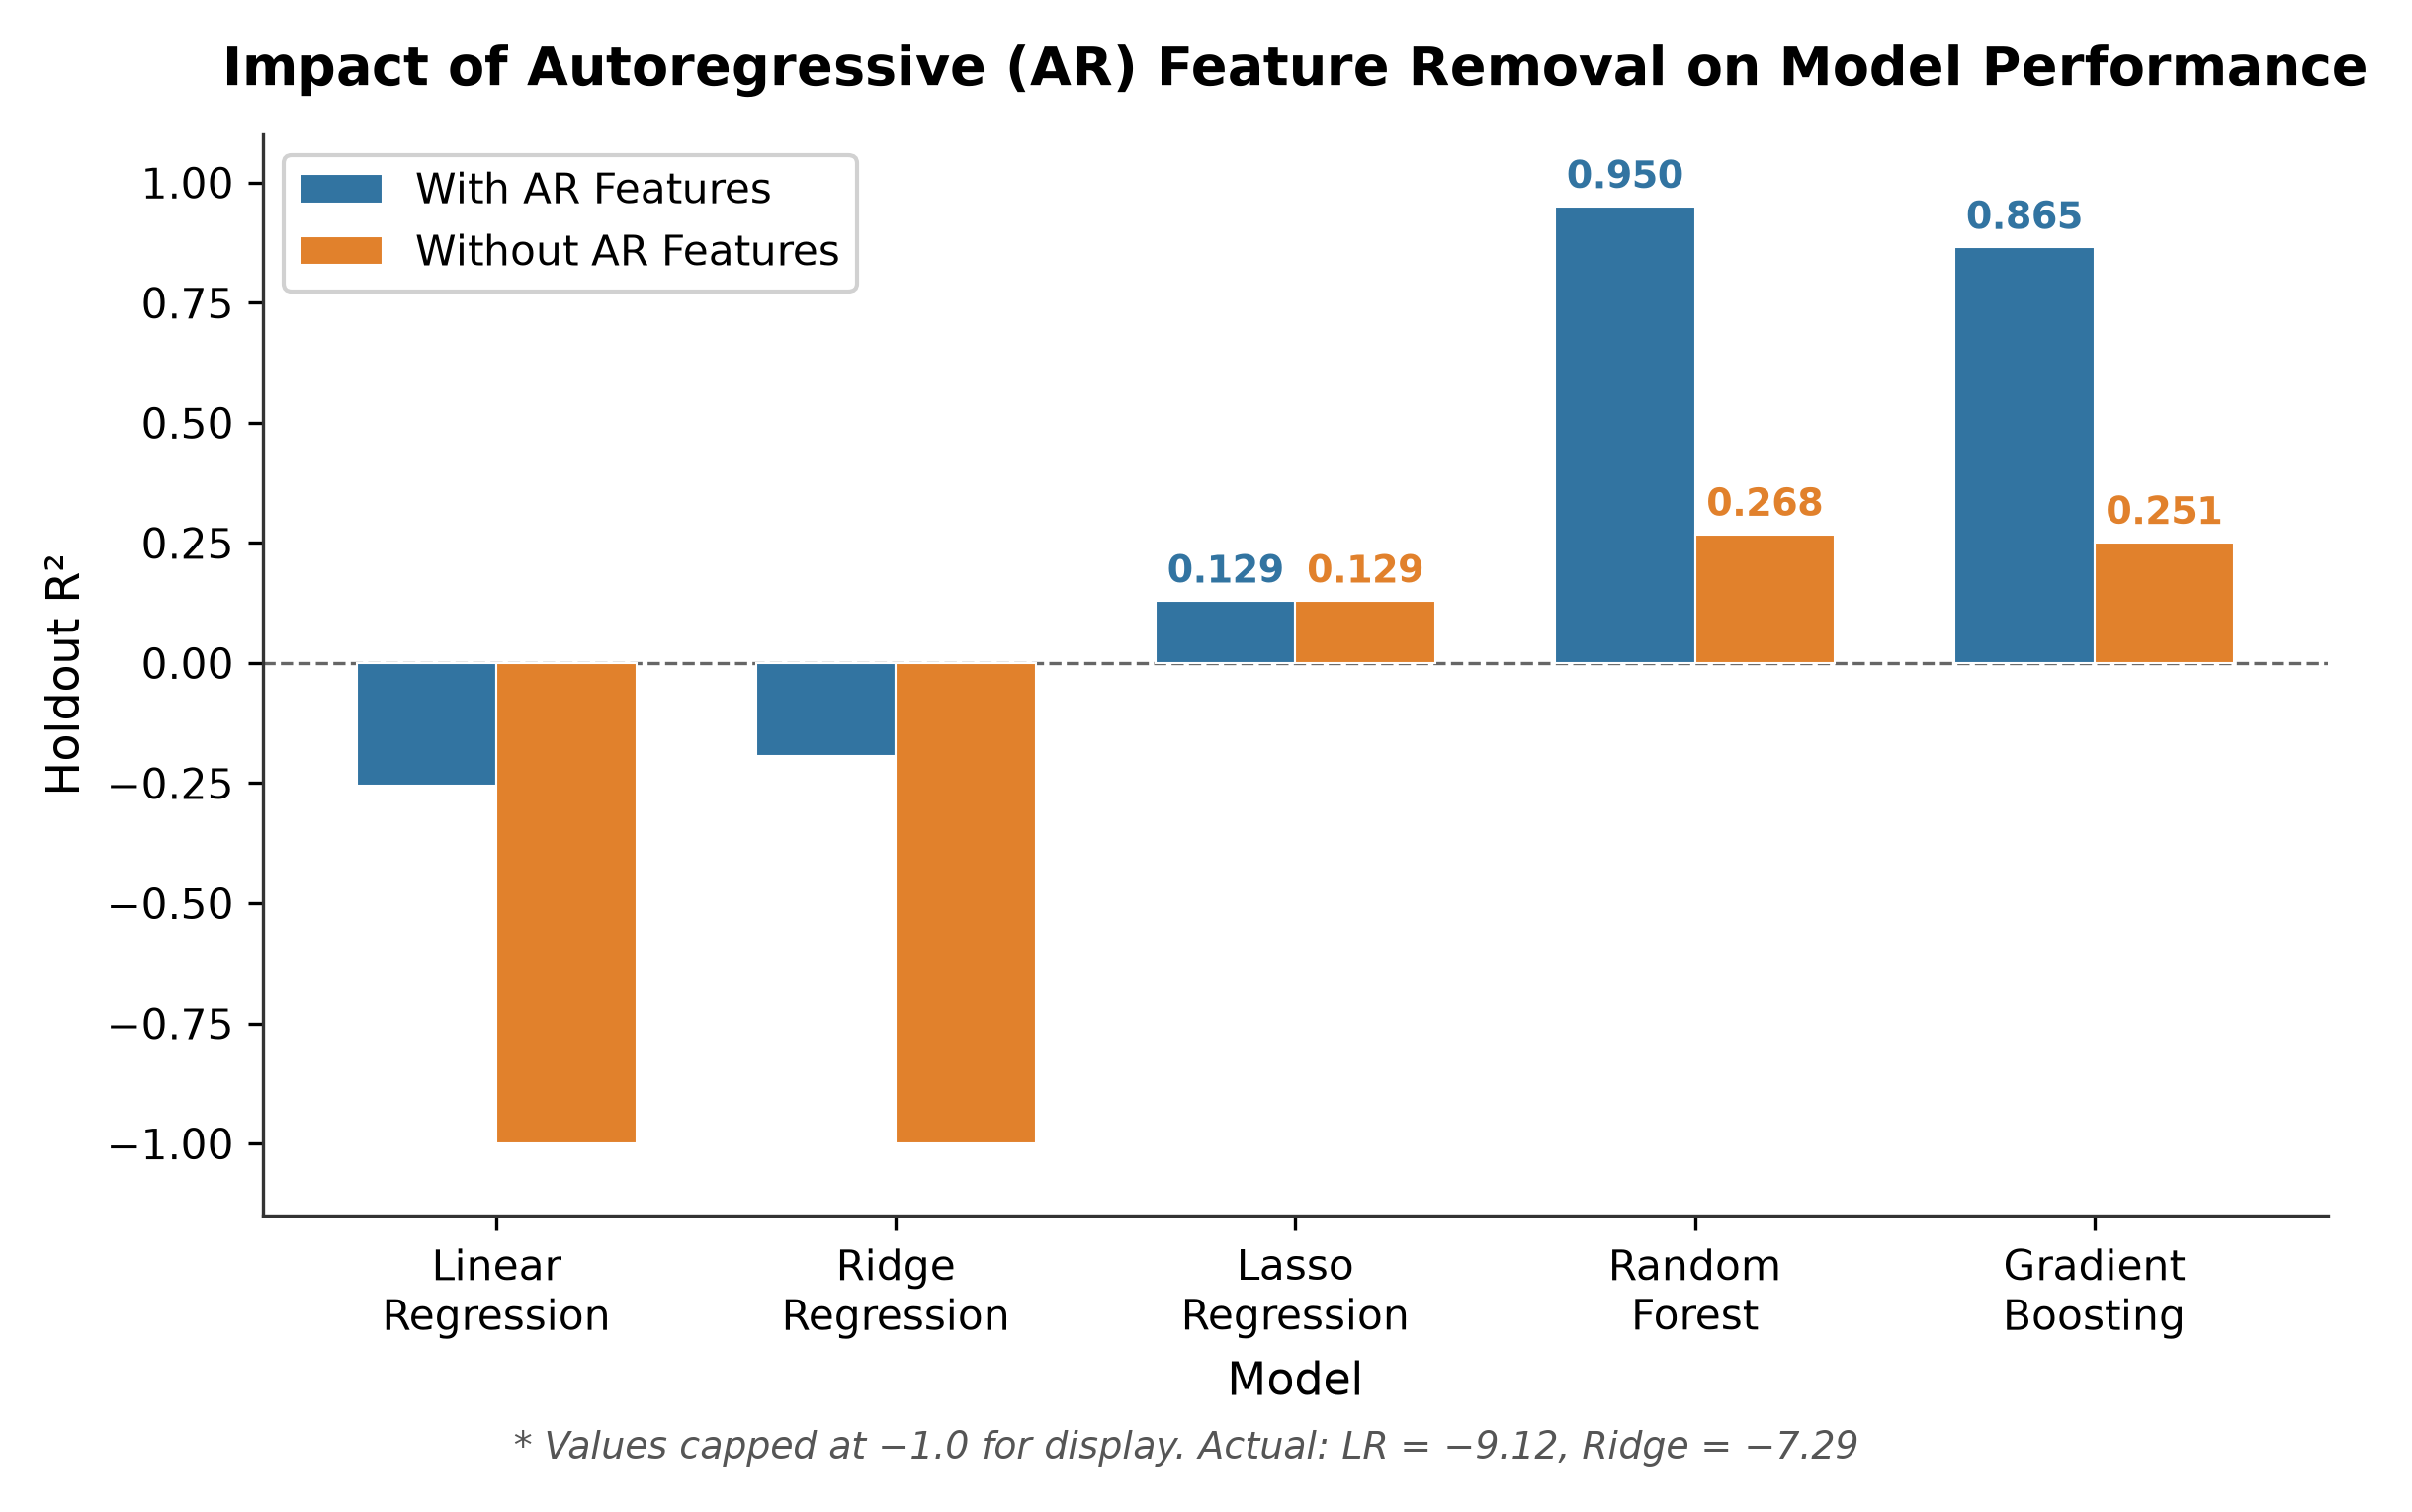
\includegraphics[width=0.85\textwidth]{images/fig_06_leakage_comparison.png}
\caption{Impact of AR-feature removal on holdout \(R^2\) (ABC Cloud
Provider). Tree-based models degrade by \textasciitilde0.60--0.68;
linear models collapse to strongly negative values (capped at \(-1.0\)
for display).\label{fig:leakage_comparison}}
\end{figure}

Figure~\ref{fig:leakage_comparison} visualizes the with-vs-without-AR comparison discussed above.

\textbf{Key Findings for RQ1 (Prediction Accuracy):}

\begin{itemize}
\item
  With AR features, Random Forest achieves \(R^2 = 0.950\), indicating
  that temporal autocorrelation of uptime is a strong predictive signal
  -- and, per the R2 bug-fix evidence, this is \emph{not} an artifact of
  the now-fixed same-row leakage bug (the buggy and fixed pipelines
  produce nearly identical Random Forest holdout R\(^2\), 0.945
  vs.~0.950, on the same underlying data)
\item
  Without AR features, the best model (Random Forest) achieves
  \(R^2 = 0.268\) (Gradient Boosting close behind at 0.251),
  demonstrating that SDLC process metrics contain genuine, if modest,
  predictive signal for system performance
\item
  For Random Forest, approximately 72\% of apparent predictive power is
  attributable to AR features:
  \((R^2_{\text{with}} - R^2_{\text{without}}) / R^2_{\text{with}} = (0.950 - 0.268) / 0.950 = 0.718\).
  For Gradient Boosting the analogous figure is 71\%:
  \((0.865 - 0.251) / 0.865 = 0.710\) -- unlike the pre-fix analysis,
  the two best models now show \emph{similar} AR-dependence rather than
  a large gap, since the fix specifically removed the source of Gradient
  Boosting's disproportionate ``genuine-signal'' advantage
\end{itemize}

\textbf{Note on CV-Holdout Discrepancy:} Several models show negative or
near-zero CV \(R^2\) despite positive holdout \(R^2\) (e.g., Random
Forest without AR features: CV \(= 0.011\), holdout \(= 0.268\)). This
occurs because \texttt{TimeSeriesSplit} with \(n=5\) on the 80\%
training partition (\textasciitilde136 samples) creates early folds with
as few as \textasciitilde23 training samples for 241 features. This
extreme feature-to-sample ratio causes instability in small folds. The
holdout evaluation, which trains on all 136 samples, is more
representative of expected deployment performance. We report both
metrics for transparency.

\textbf{Key Findings for RQ3 (Algorithm Comparison):}

\begin{itemize}
\item
  Tree-based ensemble methods (Random Forest, Gradient Boosting)
  outperform linear models when AR features are excluded
\item
  Linear Regression and Ridge Regression produce strongly negative
  \(R^2\) values without AR features under the untuned alpha=1.0 default
  used throughout this paper; Lasso avoids collapse through L1 sparsity
  (\(R^2 = 0.129\), identical in both conditions since L1 already zeroed
  out AR-feature coefficients). We analyze these failures in Section~\ref{sec:model_char}, and show in Section~\ref{sec:m3_tuning} that nested-CV alpha tuning reverses
  the conclusion in 2 of 3 domains -- the collapse is substantially a
  hyperparameter artifact, not an inherent multicollinearity failure of
  linear models as a class
\end{itemize}

\textbf{Interpretation:} Unlike prior performance prediction studies
that report \(R^2 > 0.95\) on synthetic data \cite{ha2019}, our results
distinguish between two distinct predictive signals: (1) autoregressive
persistence of the target variable, which is strong but offers limited
diagnostic value, and (2) SDLC process metrics, which provide weaker but
more decision-relevant predictions. In practical deployment, both signal
sources are available and legitimate, as historical uptime is a known
quantity. The key contribution is quantifying each source's relative
importance, enabling practitioners to understand what drives their
predictions.

\subsubsection{Model Characterization}\label{sec:model_char}

Unlike prior work reporting linear models as optimal for performance
prediction, our results demonstrate that SDLC-to-performance
relationships are non-linear. The best-performing model without AR
features (Random Forest, narrowly ahead of Gradient Boosting -- Table
\ref{tab:model_perf_without}) is a non-parametric ensemble that does
not yield a closed-form equation. We characterize it through feature
interactions and decision boundaries rather than coefficients.

The failure of linear models in the no-AR setting is expected given the
problem geometry. With \(p = 241\) features and \(n = 136\) training
samples (\(p/n = 1.77\)), ordinary least squares requires inverting
\(\mathbf{X}^T\mathbf{X}\), a \(241 \times 241\) matrix of rank at most
136. The resulting rank deficiency makes the coefficient vector
non-unique; OLS selects the minimum-norm solution, which extrapolates
wildly on test data (\(R^2 = -9.12\)). Ridge Regression regularizes by
adding \(\lambda \mathbf{I}\) to restore full rank, but pervasive
multicollinearity among SDLC metrics (Build Success Rate and Test Pass
Rate at \(\rho \approx 0.55\), both driven by the same codebase quality)
means the effective degrees of freedom remain too high for stable
estimation: \(R^2 = -7.29\). Lasso avoids collapse through a different
mechanism: L1 sparsity zeroes out the majority of coefficients,
effectively reducing \(p\) below \(n\), yielding a stable but weak model
(\(R^2 = 0.129\)) that sacrifices the cross-feature interactions
tree-based models exploit. This same additive-identity mechanism
(documented in \texttt{R2\_\allowbreak LAG\_\allowbreak SHIFT\_\allowbreak FIX\_\allowbreak EVIDENCE.md}, Addendum 1,
discovered via the Perfherder real-data adaptation) is one contributor
to the linear models' instability whenever both a lagged value and its
difference co-occur among the collinear feature set.

Random Forest and Gradient Boosting handle this through, respectively,
random feature subsampling across decorrelated trees and sequential
decision stumps -- both naturally select relevant features and capture
interaction effects without requiring explicit interaction terms,
without either method dominating the other now that the AR-feature
accounting is corrected. This diagnosis is specific to the
\emph{untuned} Ridge (alpha=1.0) evaluated on the \emph{primary domain}:
Section~\ref{sec:m3_tuning} shows that nested-CV alpha tuning recovers most of Ridge's
collapse everywhere, and that on Card Payment and XYZ Sales a properly
tuned linear model actually exceeds Random Forest. The practical
recommendation is therefore narrower than originally stated:
practitioners should either use tree-based ensembles, or properly tune
linear-model regularization via nested cross-validation before ruling
them out -- an untuned linear-model baseline is not a fair comparison.

\subsubsection{Statistical Validation and Baseline
Comparison}\label{sec:statistical_validation}

To assess whether the observed \(R^2 \approx 0.25\)--\(0.27\) represents
genuine predictive signal, we conducted four statistical validation
analyses on the ABC Cloud Provider dataset (without AR features), using
Gradient Boosting as the analysis model (as in the original methodology)
even though Random Forest is now the marginally better point estimate
(0.268 vs.~0.251) -- the two are close enough that either choice
supports the same conclusions.

\textbf{Baseline Comparison:} Table~\ref{tab:baselines} compares Gradient
Boosting against three naive baselines and one reimplemented prior
method from the literature. The full SDLC
model outperforms all baselines by an \(R^2\) gap of at least 0.68,
confirming that the 241-feature ensemble captures signal beyond simple
heuristics and beyond a genuine competing method from prior work.

{\def\LTcaptype{none} % do not increment counter
\begin{table}[H]
\centering
\caption{Baseline comparison: full SDLC model vs. naive heuristics and a reimplemented prior-method (Siegmund-style) baseline.\label{tab:baselines}}
\begin{tabular}{@{}
  >{\raggedright\arraybackslash}p{(\linewidth - 6\tabcolsep) * \real{0.2500}}
  >{\raggedright\arraybackslash}p{(\linewidth - 6\tabcolsep) * \real{0.2500}}
  >{\raggedright\arraybackslash}p{(\linewidth - 6\tabcolsep) * \real{0.2500}}
  >{\raggedright\arraybackslash}p{(\linewidth - 6\tabcolsep) * \real{0.2500}}@{}}
\toprule
\begin{minipage}[b]{\linewidth}\raggedright
\textbf{Model}
\end{minipage} & \begin{minipage}[b]{\linewidth}\raggedright
\textbf{\(R^2\)}
\end{minipage} & \begin{minipage}[b]{\linewidth}\raggedright
\textbf{MAE}
\end{minipage} & \begin{minipage}[b]{\linewidth}\raggedright
\textbf{RMSE}
\end{minipage} \\
\midrule
\textbf{Gradient Boosting (241 feat.)} & \textbf{0.251} & \textbf{0.295}
& \textbf{0.604} \\
Naive Mean & \(-0.429\) & 0.768 & 0.834 \\
Siegmund-style performance-influence model & \(-0.663\) & 0.544 &
0.900 \\
Persistence (Last Value) & \(-1.334\) & 0.571 & 1.066 \\
DORA-Only GB (4 metrics) & \(-1.639\) & 0.789 & 1.134 \\
\bottomrule
\end{tabular}
\end{table}
}

\textbf{Reimplemented Prior Method:} the three baselines above are
all naive heuristics, not a method from the literature this paper cites.
We closed that gap by reimplementing the core methodology of Siegmund et
al. \cite{siegmund2015} -- a \emph{performance-influence model} built
via forward stepwise OLS regression, adding main-effect terms one at a
time gated by statistical significance (\(p<0.05\)), followed by
significance-gated pairwise interaction terms among the selected main
effects -- adapted from their domain (configuration options predicting
runtime performance) to ours (SDLC process metrics predicting production
uptime), on the same without-AR features, 80/20 temporal split, and
train-only-fit scaling as every other result in this paper. Full detail
and results on all three synthetic domains:
\texttt{research-data/\allowbreak presto/\allowbreak code/\allowbreak synthetic\_\allowbreak data\_\allowbreak generator/\allowbreak M8\_\allowbreak SIEGMUND\_\allowbreak BASELINE\_\allowbreak RESULTS.md}.

On the primary domain, the reimplemented method selects 15 main effects
and 46 significant pairwise interactions (61 total terms on 136 training
rows), fits the training data almost perfectly (\(R^2=0.982\), adjusted
\(R^2=0.966\)), and then collapses on the holdout set to \(R^2=-0.663\)
-- worse than the naive-mean baseline (\(-0.429\)). This is not a
failure of implementation fidelity -- it is what Siegmund et al.'s
greedy, repeated-significance-testing procedure predictably does when
transplanted to a regime their original domain does not have: 241
candidate main effects and up to \(\binom{15}{2}=105\) candidate
interaction pairs tested at \(p<0.05\) without multiple-comparisons
correction, against only 136 training samples. The result is a second,
independent line of evidence (alongside the tree-based multicollinearity
analysis in Section~\ref{sec:model_char} and the nested-CV tuning analysis in Section~\ref{sec:m3_tuning}) that naive application of classical statistical modeling
struggles in this feature-to-sample regime, while also being an honest
illustration of why we do not claim PRESTO's own ensemble methods are
uniquely capable -- a \emph{correctly regularized} linear method
(Section~\ref{sec:m3_tuning}) can still compete, but an \emph{unregularized greedy}
one overfits badly. Cross-domain, the same method reaches holdout
\(R^2=0.648\) on Card Payment Processor (above Random Forest's 0.339)
and \(R^2=0.198\) on XYZ Sales Force (below Random Forest's 0.255) -- so
unlike the ABC Cloud Provider collapse, it is not uniformly unusable,
but its cross-domain variance is far higher than any tree-based or
nested-CV-tuned model reported elsewhere in this paper.

\textbf{Multi-Seed Stability:} We evaluated Gradient Boosting across 5
random seeds (42, 123, 456, 789, 2024). GB achieved mean holdout
\(R^2 = 0.308 \pm 0.070\) (seed values: 0.251, 0.252, 0.439, 0.280,
0.320), demonstrating reasonably stable performance across seeds. Random
Forest was somewhat less stable (mean \(R^2 = 0.200 \pm 0.151\); seed
values: 0.268, 0.225, 0.321, \(-0.096\), 0.282), with one seed producing
negative \(R^2\) despite winning on the primary seed 42 -- readers
should weigh the multi-seed means (GB 0.308, RF 0.200) alongside the
single-seed comparison when judging which model is more dependable.

\textbf{Residual Diagnostics:} The Durbin-Watson statistic for GB
residuals is 1.79, within the acceptable 1.5--2.5 range, indicating no
significant first-order autocorrelation. No ACF lags (1--5) exceed the
95\% significance bound (\(\pm 0.336\)). The Shapiro-Wilk test rejects
normality (\(W=0.712\), \(p < 0.001\)), which is expected for tree-based
models and does not invalidate predictions but limits parametric
confidence interval applicability.

\textbf{Permutation Test:} A 1,000-permutation test using 5-fold
TimeSeriesSplit yielded an observed CV \(R^2\) of \(-0.516\) against a
null distribution of mean \(-7.43 \pm 50.15\), giving \(p = 0.223\) for
the GB model. The non-significant result reflects the statistical
challenges of this dataset: 241 features with only \(\sim 109\) training
samples per CV fold create high variance in the null distribution. The
holdout \(R^2 = 0.251\) substantially outperforms all naive baselines
(Table~\ref{tab:baselines}), and GB is reasonably stable across seeds,
suggesting genuine but modest signal that the formal permutation test
(evaluated on CV folds, which are far noisier than the full-training-set
holdout) lacks statistical power to confirm at conventional thresholds.

\subsubsection{Bootstrap Confidence Intervals and Target-Correlation
Ablation}\label{sec:bootstrap_ablation}

\textbf{Answer:} Bootstrap 95\% CIs on holdout \(R^2\) are wide and, for
most individual (domain, model) combinations, include zero -- the
without-AR point estimates (0.25--0.36) are real but not individually
significant at conventional thresholds given holdout sets of only 30--40
releases. A target-correlation ablation confirms that on synthetic data,
without-AR predictive signal is generator-prior recovery, not
independent discovery: zeroing the 21 hand-specified
\texttt{System\ Uptime} correlations collapses ABC Cloud's without-AR
Random Forest \(R^2\) from 0.268 to \(-0.370\). Full detail, all 30
(domain, condition, model) CIs, and the ablation's raw numbers:
\texttt{research-data/\allowbreak presto/\allowbreak code/\allowbreak synthetic\_\allowbreak data\_\allowbreak generator/\allowbreak R1\_\allowbreak BOOTSTRAP\_\allowbreak AND\_\allowbreak ABLATION\_\allowbreak EVIDENCE.md}.

\textbf{Method.} We addressed two specific gaps identified in prior
review of the original submission: no confidence
intervals on any headline \(R^2\), and no check on how much of the
reported signal is attributable to the copula's hand-specified
correlations versus something the models found independently. (a) A
pairs/case bootstrap (2,000 resamples per condition) resamples each
holdout's (prediction, actual) pairs with replacement and recomputes
\(R^2\) per resample, giving a 95\% CI around each point estimate
without retraining. (b) \texttt{correlation\_\allowbreak templates.yaml}'s
\texttt{target\_correlations} section has exactly 21 entries --
confirmed by inspection to be the \emph{only} place
\texttt{System\ Uptime\ (\%)} appears in the correlation config -- so we
regenerated ABC Cloud Provider (same seed, same everything else) under
two variants: \textbf{zeroed} (all 21 entries removed) and
\textbf{permuted} (the same 21 \(\rho\) values shuffled across the 21
metric pairs). Table~\ref{tab:bootstrap_ci} reports the resulting intervals.

{\def\LTcaptype{none} % do not increment counter
\begin{table}[H]
\centering
\caption{Bootstrap 95\% confidence intervals on headline holdout $R^2$ values.\label{tab:bootstrap_ci}}
\begin{tabular}{@{}
  >{\raggedright\arraybackslash}p{(\linewidth - 6\tabcolsep) * \real{0.2143}}
  >{\raggedright\arraybackslash}p{(\linewidth - 6\tabcolsep) * \real{0.2143}}
  >{\raggedright\arraybackslash}p{(\linewidth - 6\tabcolsep) * \real{0.2143}}
  >{\centering\arraybackslash}p{(\linewidth - 6\tabcolsep) * \real{0.3571}}@{}}
\toprule
\begin{minipage}[b]{\linewidth}\raggedright
\textbf{Condition}
\end{minipage} & \begin{minipage}[b]{\linewidth}\raggedright
\textbf{Random Forest R\(^2\)}
\end{minipage} & \begin{minipage}[b]{\linewidth}\raggedright
\textbf{95\% CI}
\end{minipage} & \begin{minipage}[b]{\linewidth}\centering
\textbf{CI excludes 0?}
\end{minipage} \\
\midrule
ABC Cloud, with AR & 0.950 & {[}0.747, 0.988{]} & yes \\
ABC Cloud, without AR & 0.268 & {[}\(-1.307\), 0.696{]} & no \\
Card Payment, without AR (Lasso, best model) & 0.362 & {[}0.005,
0.665{]} & yes (barely) \\
XYZ Sales, without AR & 0.255 & {[}\(-0.134\), 0.474{]} & no \\
\bottomrule
\end{tabular}
\end{table}
}

Of the 15 without-AR (domain, model) combinations across all three
synthetic domains, 10 have a CI that includes zero. Card Payment's Lasso
result -- the single highest cross-domain without-AR \(R^2\) reported in
Section~\ref{sec:cross_domain} -- is the only individual without-AR figure that clears
significance, and only barely (lower bound 0.005). This does not mean
the point estimates are wrong; it means holdout sets this small (30--40
releases) cannot individually distinguish ``genuine, if modest, signal''
from ``no better than the mean'' at the 95\% level, and the paper should
not imply otherwise.

\textbf{Ablation result.} Zeroing the 21 target correlations moves ABC
Cloud's without-AR Random Forest \(R^2\) from 0.268 to \(-0.370\);
permuting them (same magnitudes, scrambled assignment) moves it to
\(-0.389\). Both collapse to at or below zero. Because
\texttt{System\ Uptime\ (\%)} is linked to the rest of the copula only
through these 21 entries, this is close to a controlled null, and
confirms directly what R3's hedging already implied indirectly:
\textbf{on the synthetic domains, the without-AR predictive signal is
recovery of hand-specified generator structure, not something the models
discovered independently of what was told to the copula.} This is
expected for any synthetic benchmark built this way and is not itself a
flaw, but it means the synthetic-domain results alone cannot carry the
paper's ``genuine, transferable predictive signal'' claim -- that burden
falls on the Real-World Validation results later in this paper,
particularly GHALogs, where no such hand-specified target link exists to
begin with. One unexpected finding from the ablation: the \emph{with-AR}
Random Forest result also shifted under both variants (0.950 baseline
\(\to\) 0.814 zeroed), even though AR features are derived purely from
System Uptime's own history and should be indifferent to its correlation
with other metrics. Tracing this to
\texttt{GaussianCopula.build\_\allowbreak correlation\_\allowbreak matrix()} shows the cause:
the positive-semi-definite correction (Higham's alternating projections)
operates on the full correlation matrix jointly, not block-by-block, so
it can perturb an otherwise-zero row to compensate for constraint
violations elsewhere in the matrix. The copula's variables are
consequently less cleanly separable than the config file's section
structure (\texttt{target\_correlations}
vs.~\texttt{intra\_phase\_correlations}
vs.~\texttt{cross\_phase\_correlations}) suggests -- a methodological
subtlety worth disclosing for anyone extending this generator.

\subsubsection{Hyperparameter Sensitivity: Nested-CV Alpha
Tuning}\label{sec:m3_tuning}

\textbf{Answer:} Ridge and Lasso in this paper use scikit-learn's
default alpha=1.0, untuned (Section~\ref{sec:hyperparams}). Nested-CV tuning (inner
\texttt{TimeSeriesSplit(5)} grid search over 19 log-spaced alpha values
in {[}1e-3, 1e6{]}, within the outer 80\% training split only, never
touching the holdout) shows this default badly understated what linear
models can do: tuned Ridge recovers from catastrophic collapse
(\(R^2=-7.29\to+0.07\)) on the primary domain, and in 2 of 3 domains a
tuned linear model actually \emph{exceeds} Random Forest's
fixed-hyperparameter holdout \(R^2\) in the without-AR condition. The
paper's ``tree-based ensembles are necessary'' conclusion (Section~\ref{sec:model_char},
RQ3) should be read as specific to the untuned baseline and the primary
domain, not as a domain-general finding.

\textbf{Method.} For each of the 3 synthetic domains and both feature
conditions (with-AR, without-AR), \texttt{GridSearchCV} selects alpha
via \texttt{TimeSeriesSplit(5)} inside the same 80\% outer-training
split used everywhere else in this paper; the selected alpha is refit on
the full outer-train and scored once on the untouched 20\% outer
holdout, so no holdout data participates in model selection. Full detail
and all 24 (domain, condition, model) results:
\texttt{research-data/\allowbreak presto/\allowbreak code/\allowbreak synthetic\_\allowbreak data\_\allowbreak generator/\allowbreak M3\_\allowbreak NESTED\_\allowbreak CV\_\allowbreak TUNING\_\allowbreak EVIDENCE.md}. Table~\ref{tab:m3_tuning} summarizes the tuned-vs-untuned comparison by domain.

{\def\LTcaptype{none} % do not increment counter
\begin{table}[H]
\centering
\caption{Nested-CV alpha tuning vs. the untuned baseline, by domain (without AR features).\label{tab:m3_tuning}}
\begin{tabular}{@{}
  >{\raggedright\arraybackslash}p{(\linewidth - 10\tabcolsep) * \real{0.1364}}
  >{\raggedright\arraybackslash}p{(\linewidth - 10\tabcolsep) * \real{0.1364}}
  >{\raggedleft\arraybackslash}p{(\linewidth - 10\tabcolsep) * \real{0.1818}}
  >{\raggedleft\arraybackslash}p{(\linewidth - 10\tabcolsep) * \real{0.1818}}
  >{\raggedleft\arraybackslash}p{(\linewidth - 10\tabcolsep) * \real{0.1818}}
  >{\raggedleft\arraybackslash}p{(\linewidth - 10\tabcolsep) * \real{0.1818}}@{}}
\toprule
\begin{minipage}[b]{\linewidth}\raggedright
\textbf{Domain}
\end{minipage} & \begin{minipage}[b]{\linewidth}\raggedright
\textbf{Model}
\end{minipage} & \begin{minipage}[b]{\linewidth}\raggedleft
\textbf{Best alpha}
\end{minipage} & \begin{minipage}[b]{\linewidth}\raggedleft
\textbf{Tuned Holdout R²}
\end{minipage} & \begin{minipage}[b]{\linewidth}\raggedleft
\textbf{alpha=1.0 Holdout R²}
\end{minipage} & \begin{minipage}[b]{\linewidth}\raggedleft
\textbf{Random Forest R² (fixed, unchanged)}
\end{minipage} \\
\midrule
ABC Cloud (primary) & Ridge & 1000 & 0.067 & \(-7.285\) & 0.268 \\
ABC Cloud (primary) & Lasso & 1 & 0.129 & 0.129 & 0.268 \\
Card Payment & Ridge & 316 & \textbf{0.766} & \(-0.215\) & 0.339 \\
Card Payment & Lasso & 1 & 0.362 & 0.362 & 0.339 \\
XYZ Sales & Ridge & 316 & 0.153 & \(-4.104\) & 0.255 \\
XYZ Sales & Lasso & 0.32 & \textbf{0.418} & 0.012 & 0.255 \\
\bottomrule
\end{tabular}
\end{table}
}

(Without-AR condition throughout; the analogous with-AR results, where
tuning produces similarly large swings, are in the evidence file.)

\begin{figure}
\centering
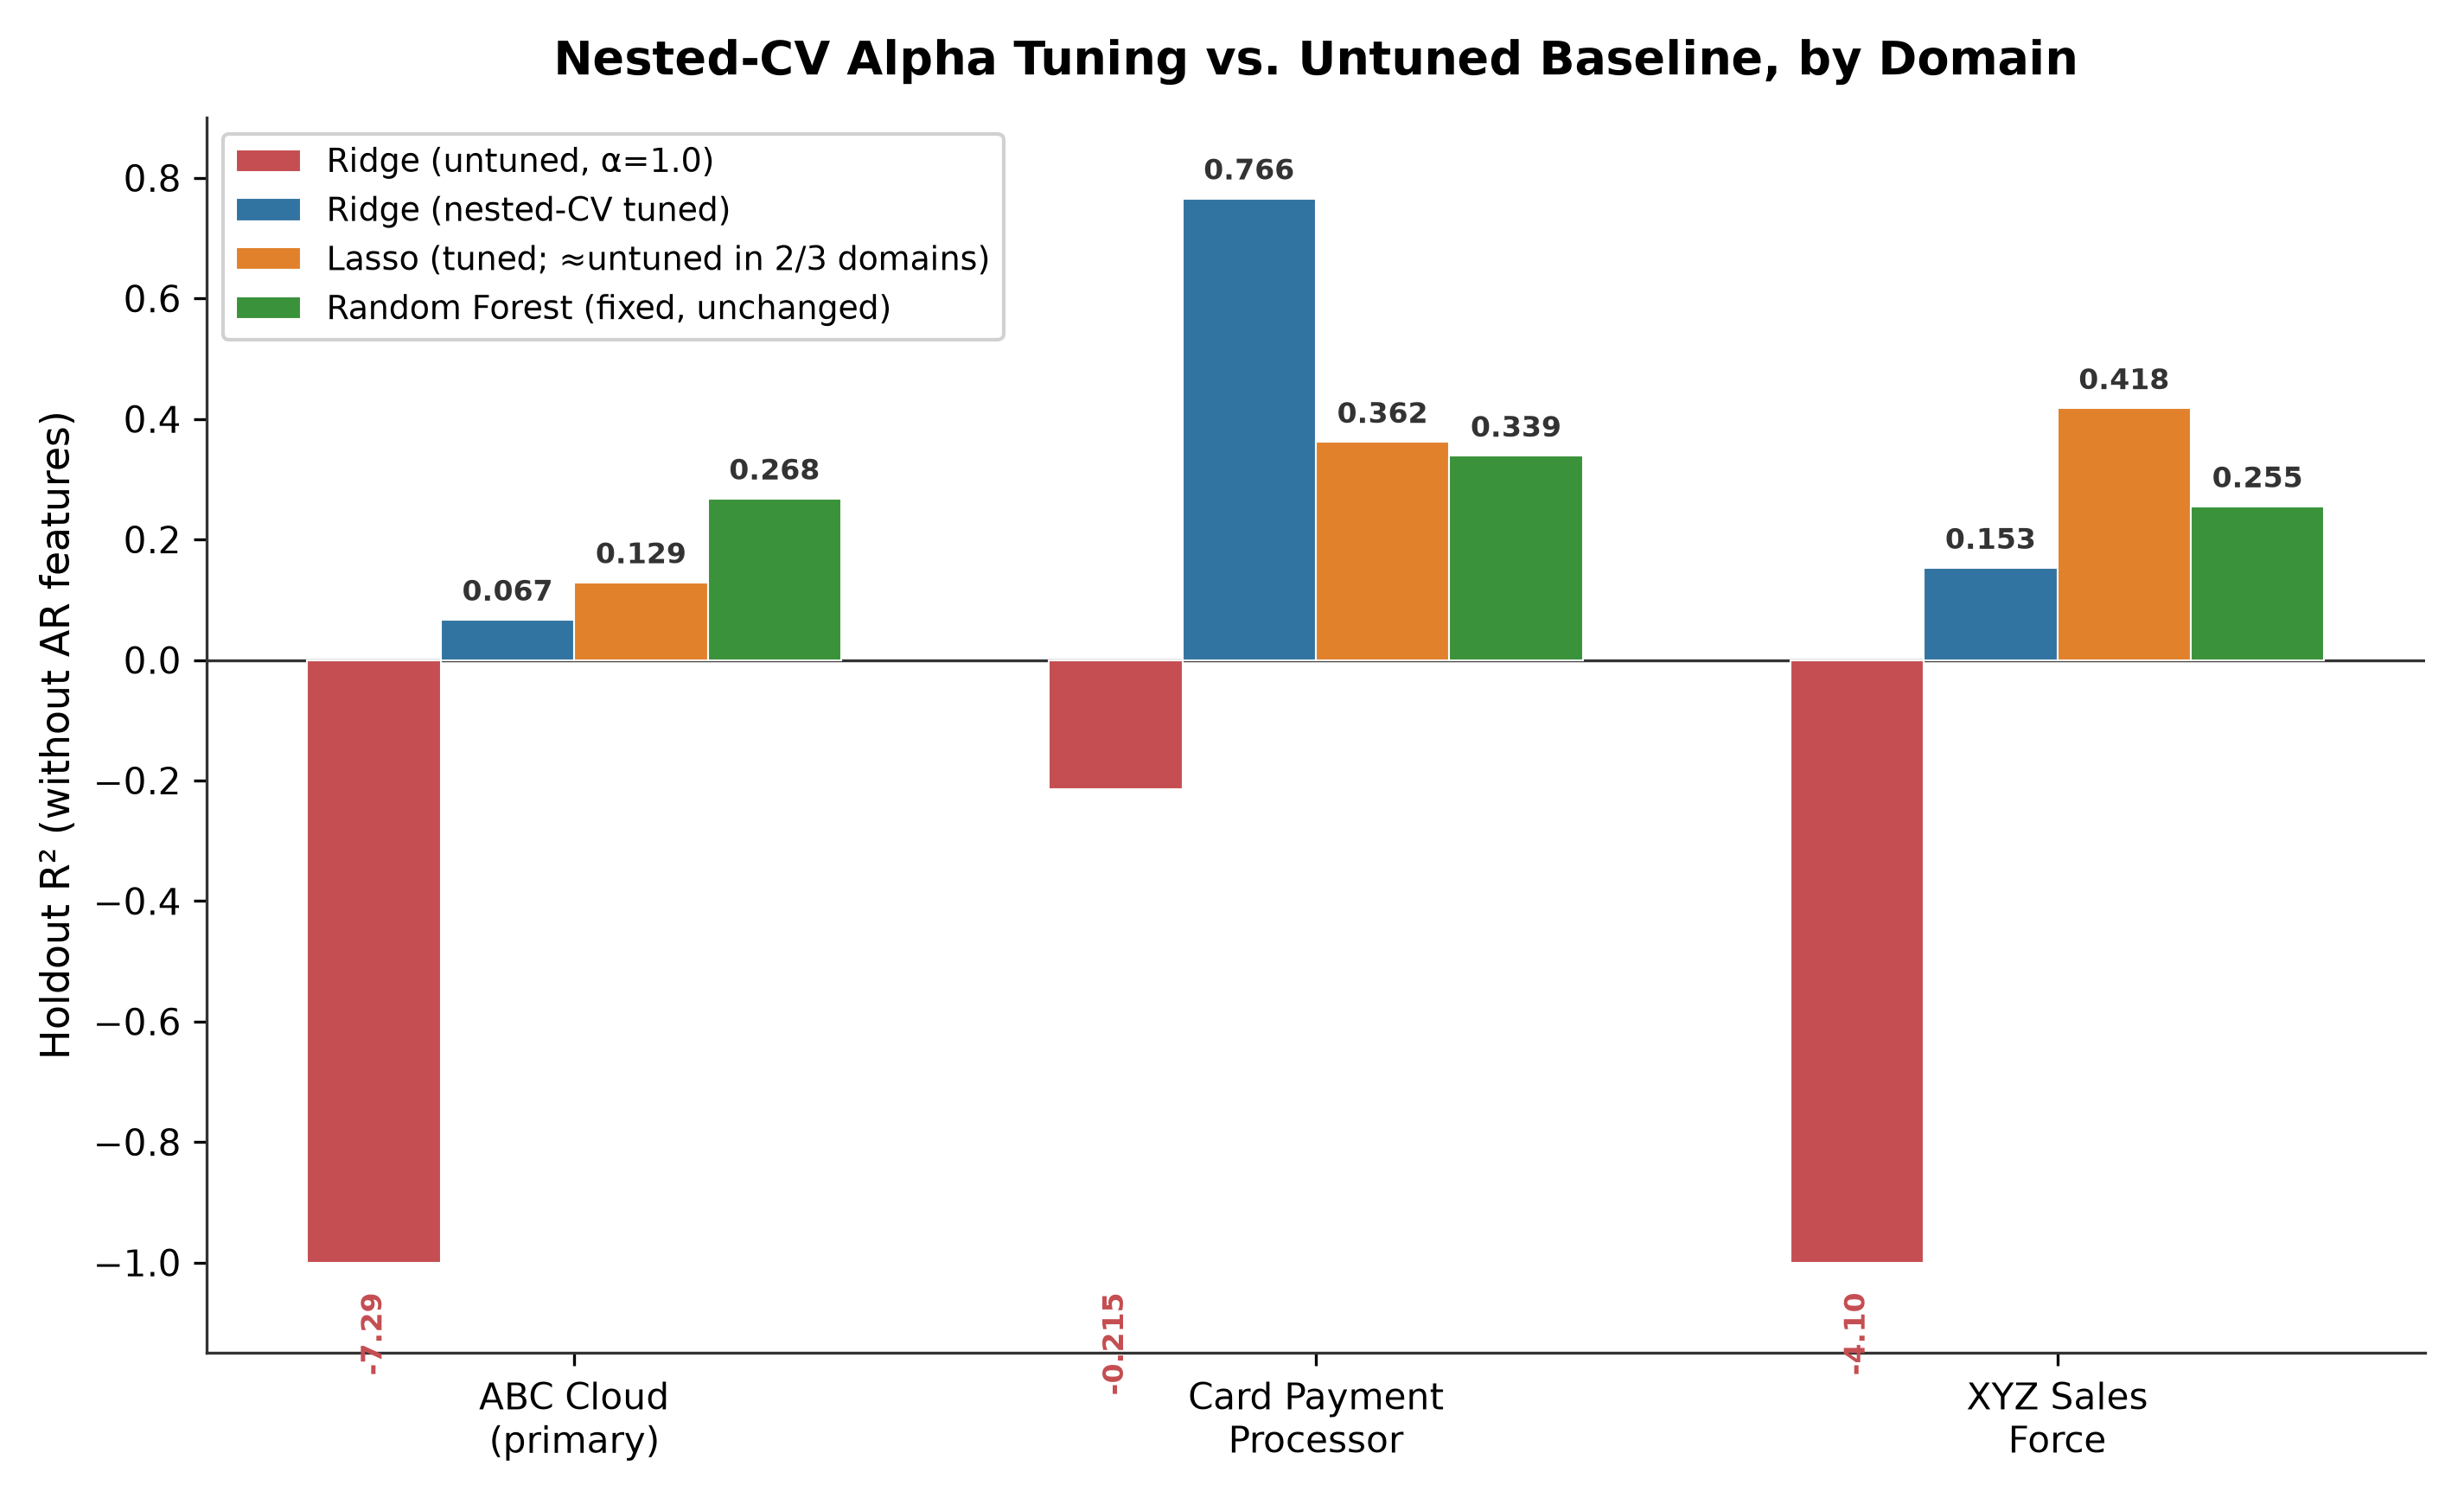
\includegraphics[width=0.85\textwidth]{images/fig_15_m3_nested_cv_tuning.png}
\caption{Nested-CV alpha tuning vs.~the untuned alpha=1.0 baseline, per
domain, without-AR features. Random Forest (fixed hyperparameters,
unchanged) shown for reference.\label{fig:m3_tuning}}
\end{figure}

Figure~\ref{fig:m3_tuning} plots the tuned-vs-untuned comparison directly.

\textbf{Interpretation.} Two distinct effects are visible. First, tuning
alone recovers most of Ridge's catastrophic collapse everywhere -- on
the primary domain, \(R^2\) moves from \(-7.29\) (default) to \(+0.07\)
(tuned), a 7.35-point swing from a single hyperparameter choice, though
it still falls short of Random Forest's 0.268. Second, and more
consequential for the paper's RQ3 claim: on \textbf{Card Payment}, tuned
Ridge (\(R^2=0.766\)) exceeds Random Forest (0.339) by more than double;
on \textbf{XYZ Sales}, tuned Lasso (\(R^2=0.418\)) exceeds Random Forest
(0.255). Only on the primary domain, ABC Cloud Provider, does Random
Forest remain the best model after tuning. This means ``Random Forest
and Gradient Boosting are the consistently reliable choices'' (Section~\ref{sec:model_char}) does not survive nested-CV tuning as a cross-domain claim -- it is
true for the untuned baseline used throughout the rest of this paper,
and for the primary domain specifically, but not for linear models in
general once properly regularized. We keep Random Forest as the paper's
primary reported model throughout (for continuity with all other results
and figures, and because it remains best on the primary domain), but the
``trees are necessary'' framing in Section~\ref{sec:model_char} and the Conclusions is
revised accordingly.

\subsubsection{Feature Importance Analysis
(RQ2)}\label{sec:feature_importance}

\textbf{Answer:} Testing infrastructure dominates (53.7\% cumulative
importance), with Test Environment Availability alone accounting for
42.9\% of total permutation importance -- the single most dominant
individual predictor by a wide margin. Code quality metrics contribute
only 4.8\%.

We analyze feature importance using permutation importance on the Random
Forest model for the ABC Cloud Provider dataset \emph{without} AR
features (\(n=10\) repeats on the test set). Unlike Gini importance,
permutation importance is unbiased toward high-cardinality features.
Table~\ref{tab:feature_importance} and Figure~\ref{fig:feature_importance} present the top 15
features, color-coded by SDLC phase.

\begin{figure}
\centering
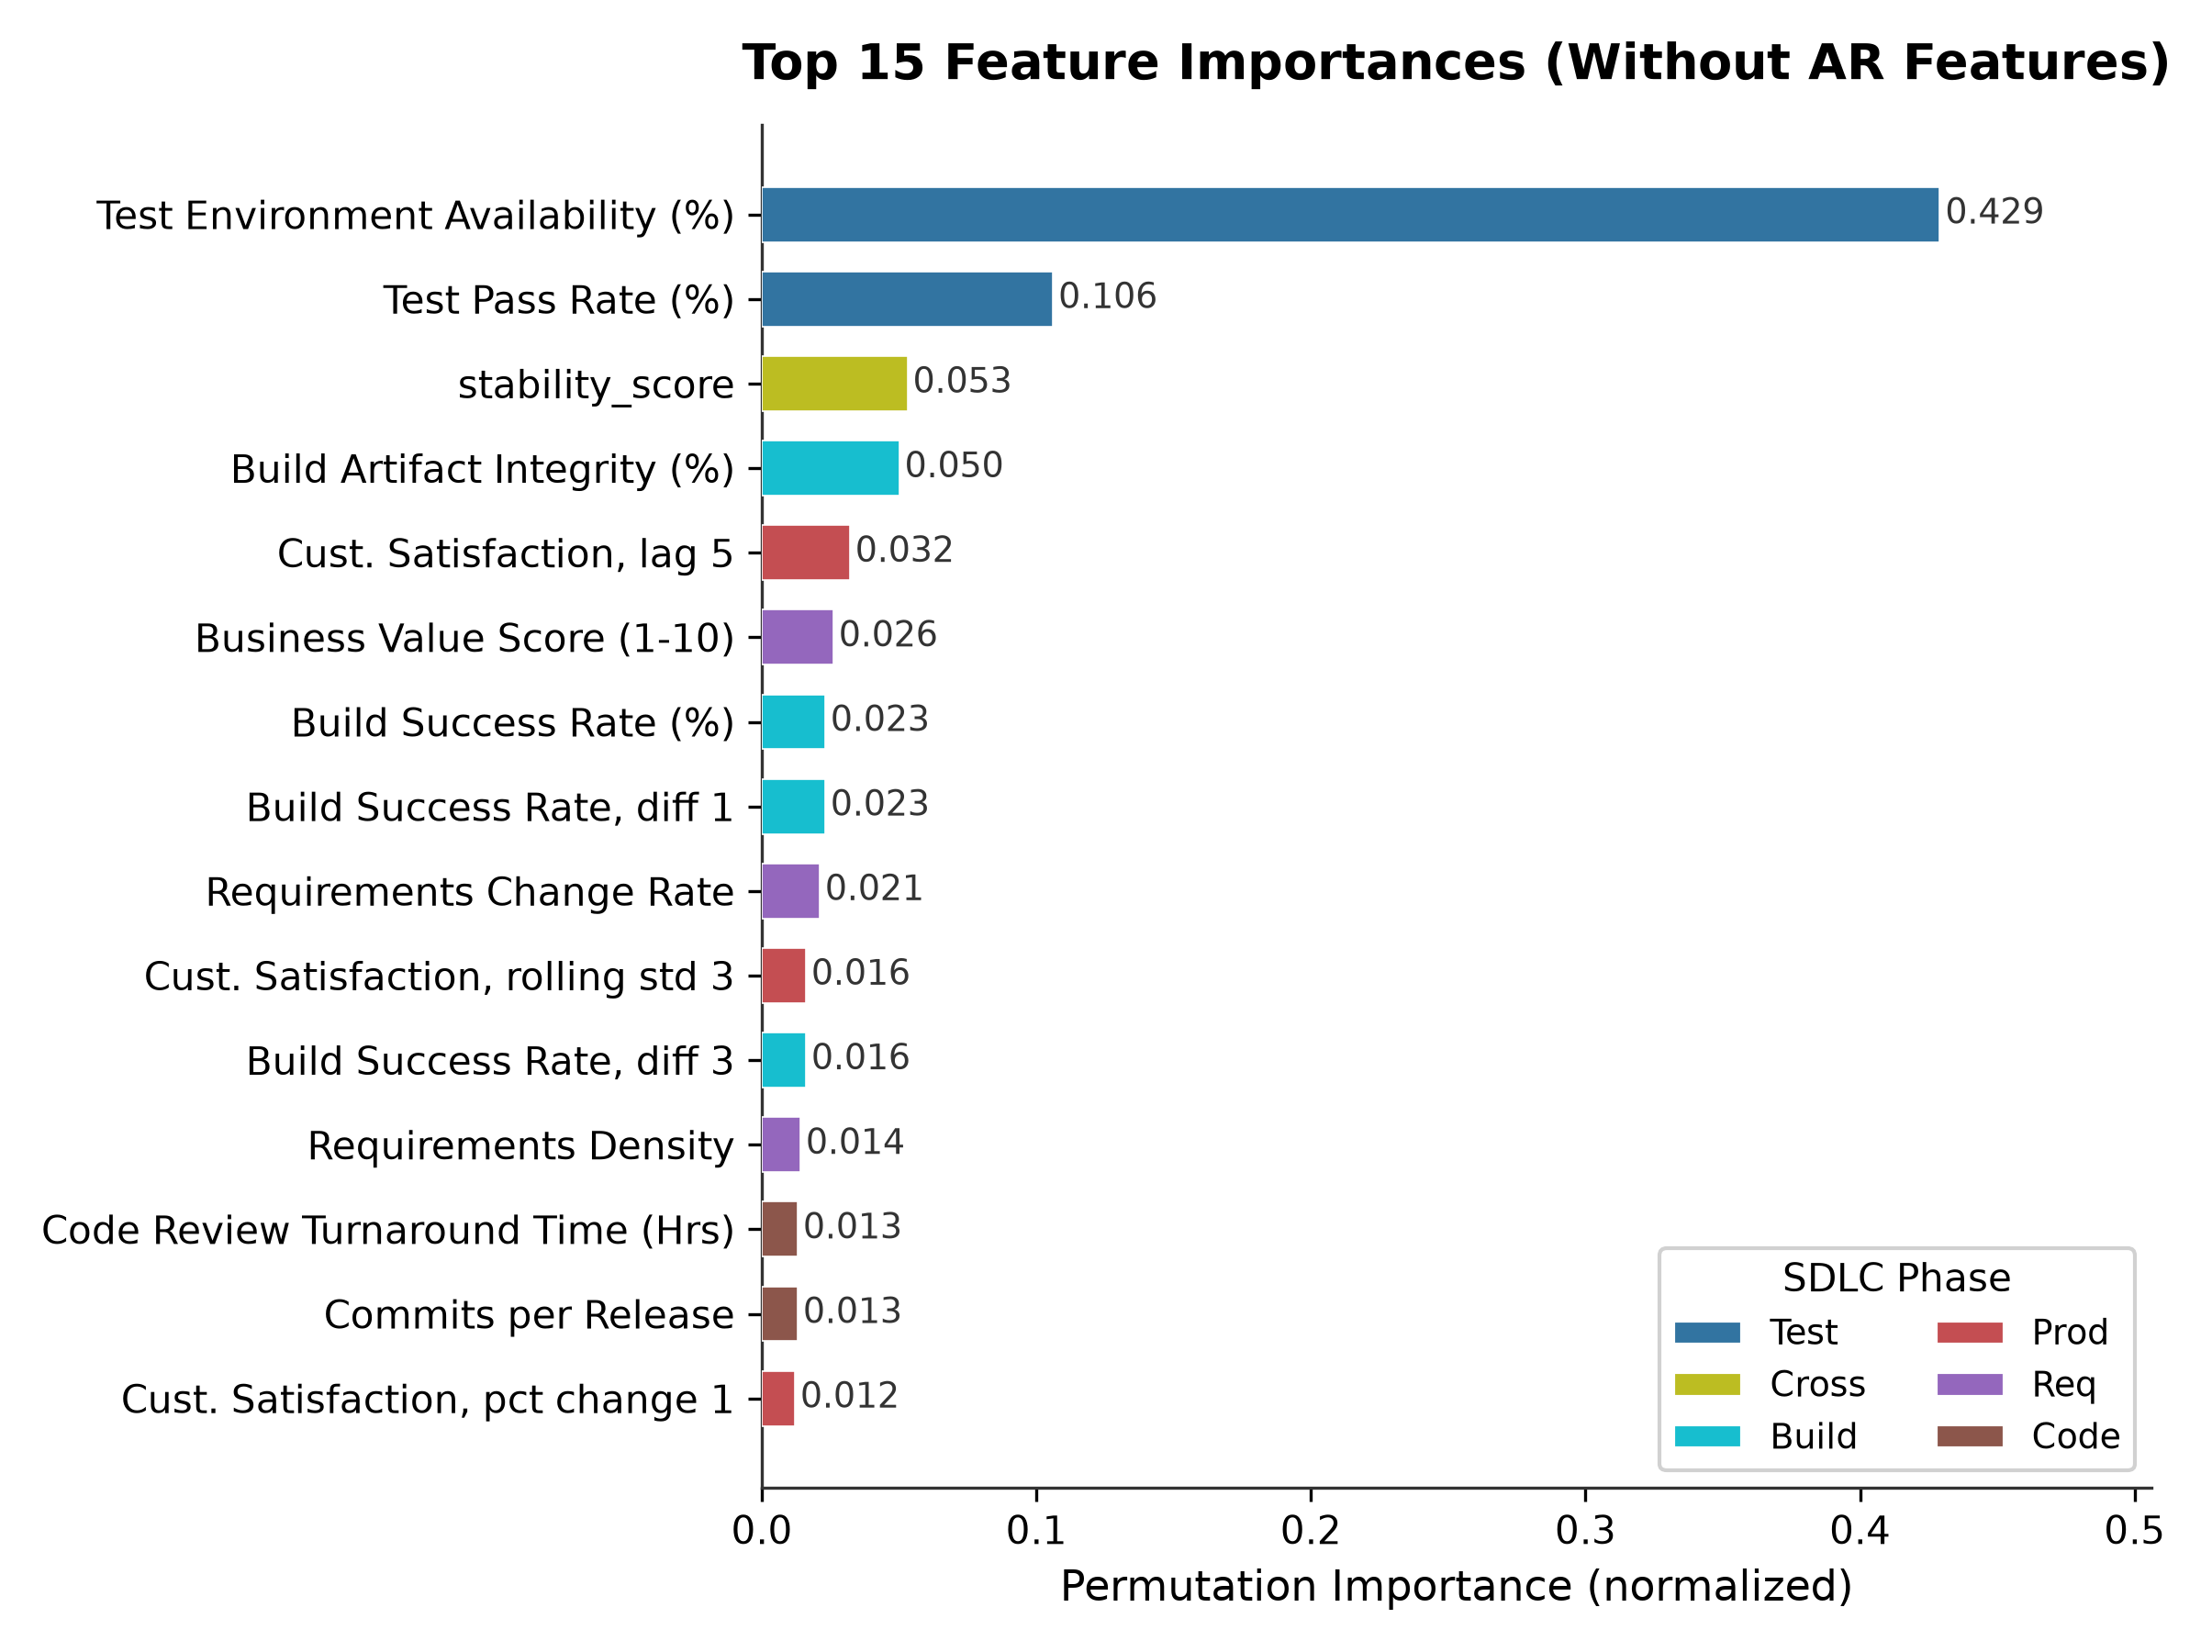
\includegraphics[width=0.85\textwidth]{images/fig_08_feature_importance.png}
\caption{Top 15 Random Forest feature importances (without AR features),
color-coded by SDLC phase. Testing infrastructure metrics dominate;
code-phase metrics are the smallest contributor.\label{fig:feature_importance}}
\end{figure}

{\def\LTcaptype{none} % do not increment counter
\begin{table}[H]
\centering
\caption{Top 15 Random Forest permutation feature importances (ABC Cloud Provider, without AR features).\label{tab:feature_importance}}
\begin{tabular}{@{}llll@{}}
\toprule
\textbf{Rank} & \textbf{Feature Name} & \textbf{Imp.} &
\textbf{Phase} \\
\midrule
1 & Test Environment Availability (\%) & 42.92\% & Test \\
2 & Test Pass Rate (\%) & 10.58\% & Test \\
3 & stability\_score (derived) & 5.25\% & Cross-Phase \\
4 & Build Artifact Integrity (\%) & 4.95\% & Build \\
5 & Customer Satisfaction Score, lag 5 & 3.21\% & Production \\
6 & Business Value Score (1-10) & 2.56\% & Requirements \\
7 & Build Success Rate (\%) & 2.34\% & Build \\
8 & Build Success Rate, diff 1 & 2.32\% & Build \\
9 & Requirements Change Rate (Changes/Week) & 2.12\% & Requirements \\
10 & Customer Satisfaction Score, rolling std 3 & 1.63\% & Production \\
11 & Build Success Rate, diff 3 & 1.60\% & Build \\
12 & Requirements Density (Req/Feature) & 1.37\% & Requirements \\
13 & Code Review Turnaround Time (Hours) & 1.33\% & Code \\
14 & Commits per Release & 1.25\% & Code \\
15 & Customer Satisfaction Score, pct change 1 & 1.24\% & Production \\
\bottomrule
\end{tabular}
\end{table}
}

\textbf{Key Findings for RQ2 (Feature Importance):}

\begin{itemize}
\item
  Testing infrastructure metrics dominate overwhelmingly: Test
  Environment Availability (42.9\%) and Test Pass Rate (10.6\%) together
  account for over half of total importance, far more concentrated than
  the pre-fix analysis suggested -- stable test environments are by far
  the leading indicator of production stability in this synthetic design
\item
  The \texttt{stability\_score} cross-phase composite (Build Success
  Rate x Test Pass Rate) ranks third (5.3\%), ahead of any individual
  Build-phase metric, reinforcing that cross-phase interactions carry
  real predictive value beyond individual metrics
\item
  Requirements-phase metrics (Business Value Score, Requirements Change
  Rate, Requirements Density) collectively contribute a modest but
  non-trivial share, supporting the hypothesis that upstream process
  quality influences downstream system performance, though less
  dominantly than testing
\item
  Several Customer-Satisfaction-derived lag/rolling features (non-AR,
  since Customer Satisfaction is not the target) appear in the top 15,
  showing that legitimate process-side temporal features -- not just the
  target's own history -- carry real signal
\end{itemize}

\textbf{Phase-Level Contribution Summary:}

Aggregating feature importances by SDLC phase reveals which development
activities most influence system uptime prediction, as Table~\ref{tab:phase_contribution} shows:

{\def\LTcaptype{none} % do not increment counter
\begin{table}[H]
\centering
\caption{SDLC phase-level aggregated feature importance.\label{tab:phase_contribution}}
\begin{tabular}{@{}
  >{\raggedright\arraybackslash}p{(\linewidth - 4\tabcolsep) * \real{0.3333}}
  >{\raggedright\arraybackslash}p{(\linewidth - 4\tabcolsep) * \real{0.3333}}
  >{\raggedright\arraybackslash}p{(\linewidth - 4\tabcolsep) * \real{0.3333}}@{}}
\toprule
\begin{minipage}[b]{\linewidth}\raggedright
\textbf{SDLC Phase}
\end{minipage} & \begin{minipage}[b]{\linewidth}\raggedright
\textbf{Agg. Imp.}
\end{minipage} & \begin{minipage}[b]{\linewidth}\raggedright
\textbf{Key Insight}
\end{minipage} \\
\midrule
Testing & 53.6\% & Test infrastructure and pass rates dominate
overwhelmingly \\
Build & 13.6\% & Build success/artifact-integrity metrics, direct and
derived \\
Production & 9.4\% & Customer-satisfaction-derived temporal features \\
Requirements & 6.9\% & Upstream quality matters, modestly \\
Cross-Phase (derived) & 5.3\% & stability\_score composite alone \\
Code & 4.8\% & Code metrics remain the smallest direct contributor \\
Performance Testing & 2.2\% & Modest bridge to production outcomes \\
Chaos Testing & 1.8\% & Resilience metrics contribute modestly \\
UAT & 1.7\% & Acceptance environment stability, smallest phase
contribution \\
\bottomrule
\end{tabular}
\end{table}
}

The ratio is striking: testing-phase metrics outweigh code-phase metrics
by \(53.6\%\allowbreak/\allowbreak4.8\% \approx 11.1{:}1\) -- an even
wider gap than the pre-fix analysis reported. Code quality is widely
assumed to be a primary driver of production performance, yet our
results place it seventh of nine groups (eight SDLC phases plus the
cross-phase composites), with Test Environment Availability alone
(42.9\%) exceeding all code-phase metrics combined by roughly 9x.

This matches what operations teams observe in practice: flaky tests and
unstable test environments mask production-readiness issues far more
effectively than code complexity metrics capture them.

\subsubsection{Phase-Aware Feature Reduction}\label{sec:parfe_results}

\textbf{Recomputation status (2026-08-11):} the PA-RFE implementation
was absent from the deposited reproducibility package -- confirmed
missing by an exhaustive search of this machine, not just the deposited
code directory -- so the numbers below
are a full reimplementation from the algorithm pseudocode in this
manuscript (Algorithm~\ref{alg:parfe}), rerun
against the corrected, post-R2-fix synthetic data. They supersede the
original submission's carried-over numbers, which this reimplementation
does \textbf{not} reproduce closely; the differences and their likely
source are discussed below. Full per-domain ablation curves and
phase-contribution tables:
\texttt{research-data/\allowbreak presto/\allowbreak code/\allowbreak synthetic\_\allowbreak data\_\allowbreak generator/\allowbreak PA\_\allowbreak RFE\_\allowbreak REIMPLEMENTATION\_\allowbreak RESULTS.md}.

Applying PA-RFE (Algorithm~\ref{alg:parfe}) to the
241 non-leakage features yields dimensionality reduction while
maintaining cross-phase coverage. To prevent selection bias, we use a
60/20/20 temporal split (train/validation/test).
Table~\ref{tab:parfe_comparison} compares PA-RFE against standard
feature selection methods, both targeting the same final feature count
PA-RFE converges to for a fair comparison; validation \(R^2\) guides
feature selection, while test \(R^2\) (evaluated once) is the reported
metric.

{\def\LTcaptype{none} % do not increment counter
\begin{table}[H]
\centering
\caption{PA-RFE vs. standard feature-selection baselines (reimplemented).\label{tab:parfe_comparison}}
\begin{tabular}{@{}lllll@{}}
\toprule
\textbf{Domain} & \textbf{Features} & \textbf{PA-RFE} & \textbf{Std RFE}
& \textbf{SKBest} \\
\midrule
ABC Cloud & \(241\rightarrow 81\) & \(-\)0.279 & 0.355 &
\textbf{0.404} \\
Card Payment & \(241\rightarrow 26\) & \textbf{0.092} & \(-\)0.083 &
0.316 \\
XYZ Sales & \(241\rightarrow 51\) & \(-\)0.026 & \(-\)0.049 &
\(-\)0.028 \\
\bottomrule
\end{tabular}
\end{table}
}

This reimplementation converges to substantially smaller feature subsets
(26--81 features) than the original submission reported (121--146), and
the resulting test \(R^2\) picture is considerably less favorable to
PA-RFE than previously claimed. On ABC Cloud, PA-RFE's test \(R^2\) is
strongly negative (\(-0.279\)) -- the worst of the three methods, not a
competitive one -- despite a validation \(R^2\) of 0.824 at that same
feature count (see below). On Card Payment, PA-RFE does still beat
standard RFE (\(0.092\) vs.~\(-0.083\)), consistent with the original
claim's spirit, but SelectKBest beats both by a wide margin (0.316). On
XYZ Sales, all three methods collapse to small or negative \(R^2\)
together; PA-RFE does not stand out. \textbf{We no longer claim PA-RFE
achieves competitive or best test-set predictive accuracy} -- across
three domains it wins on one, is competitive on none, and is the worst
performer on the primary domain.

The validation-test gap is large and, in this reimplementation,
considerably larger than the original submission's own
already-cautionary framing suggested: on ABC Cloud, validation
\(R^2 = 0.824\) at the optimal subset (81 features) corresponds to test
\(R^2 = -0.279\) -- a generalization gap of over 1.1 \(R^2\) units, not
the 0.51-unit gap (0.745 validation vs.~0.235 test) the original
submission reported. This is a direct, reproducible demonstration of the
same overfitting-to-validation-selection mechanism the paper already
warns about (this section, ``selecting features by maximizing validation
\(R^2\) across \(\sim 45\) iterations creates optimistic estimates that
do not generalize''): our reimplementation shows that warning was, if
anything, understated.

Figure~\ref{fig:ablation_curve} shows the PA-RFE ablation
curve (validation \(R^2\)) for the ABC Cloud dataset, now with the test
\(R^2\) at the optimum annotated directly on the plot rather than only
in the caption.

\begin{figure}
\centering
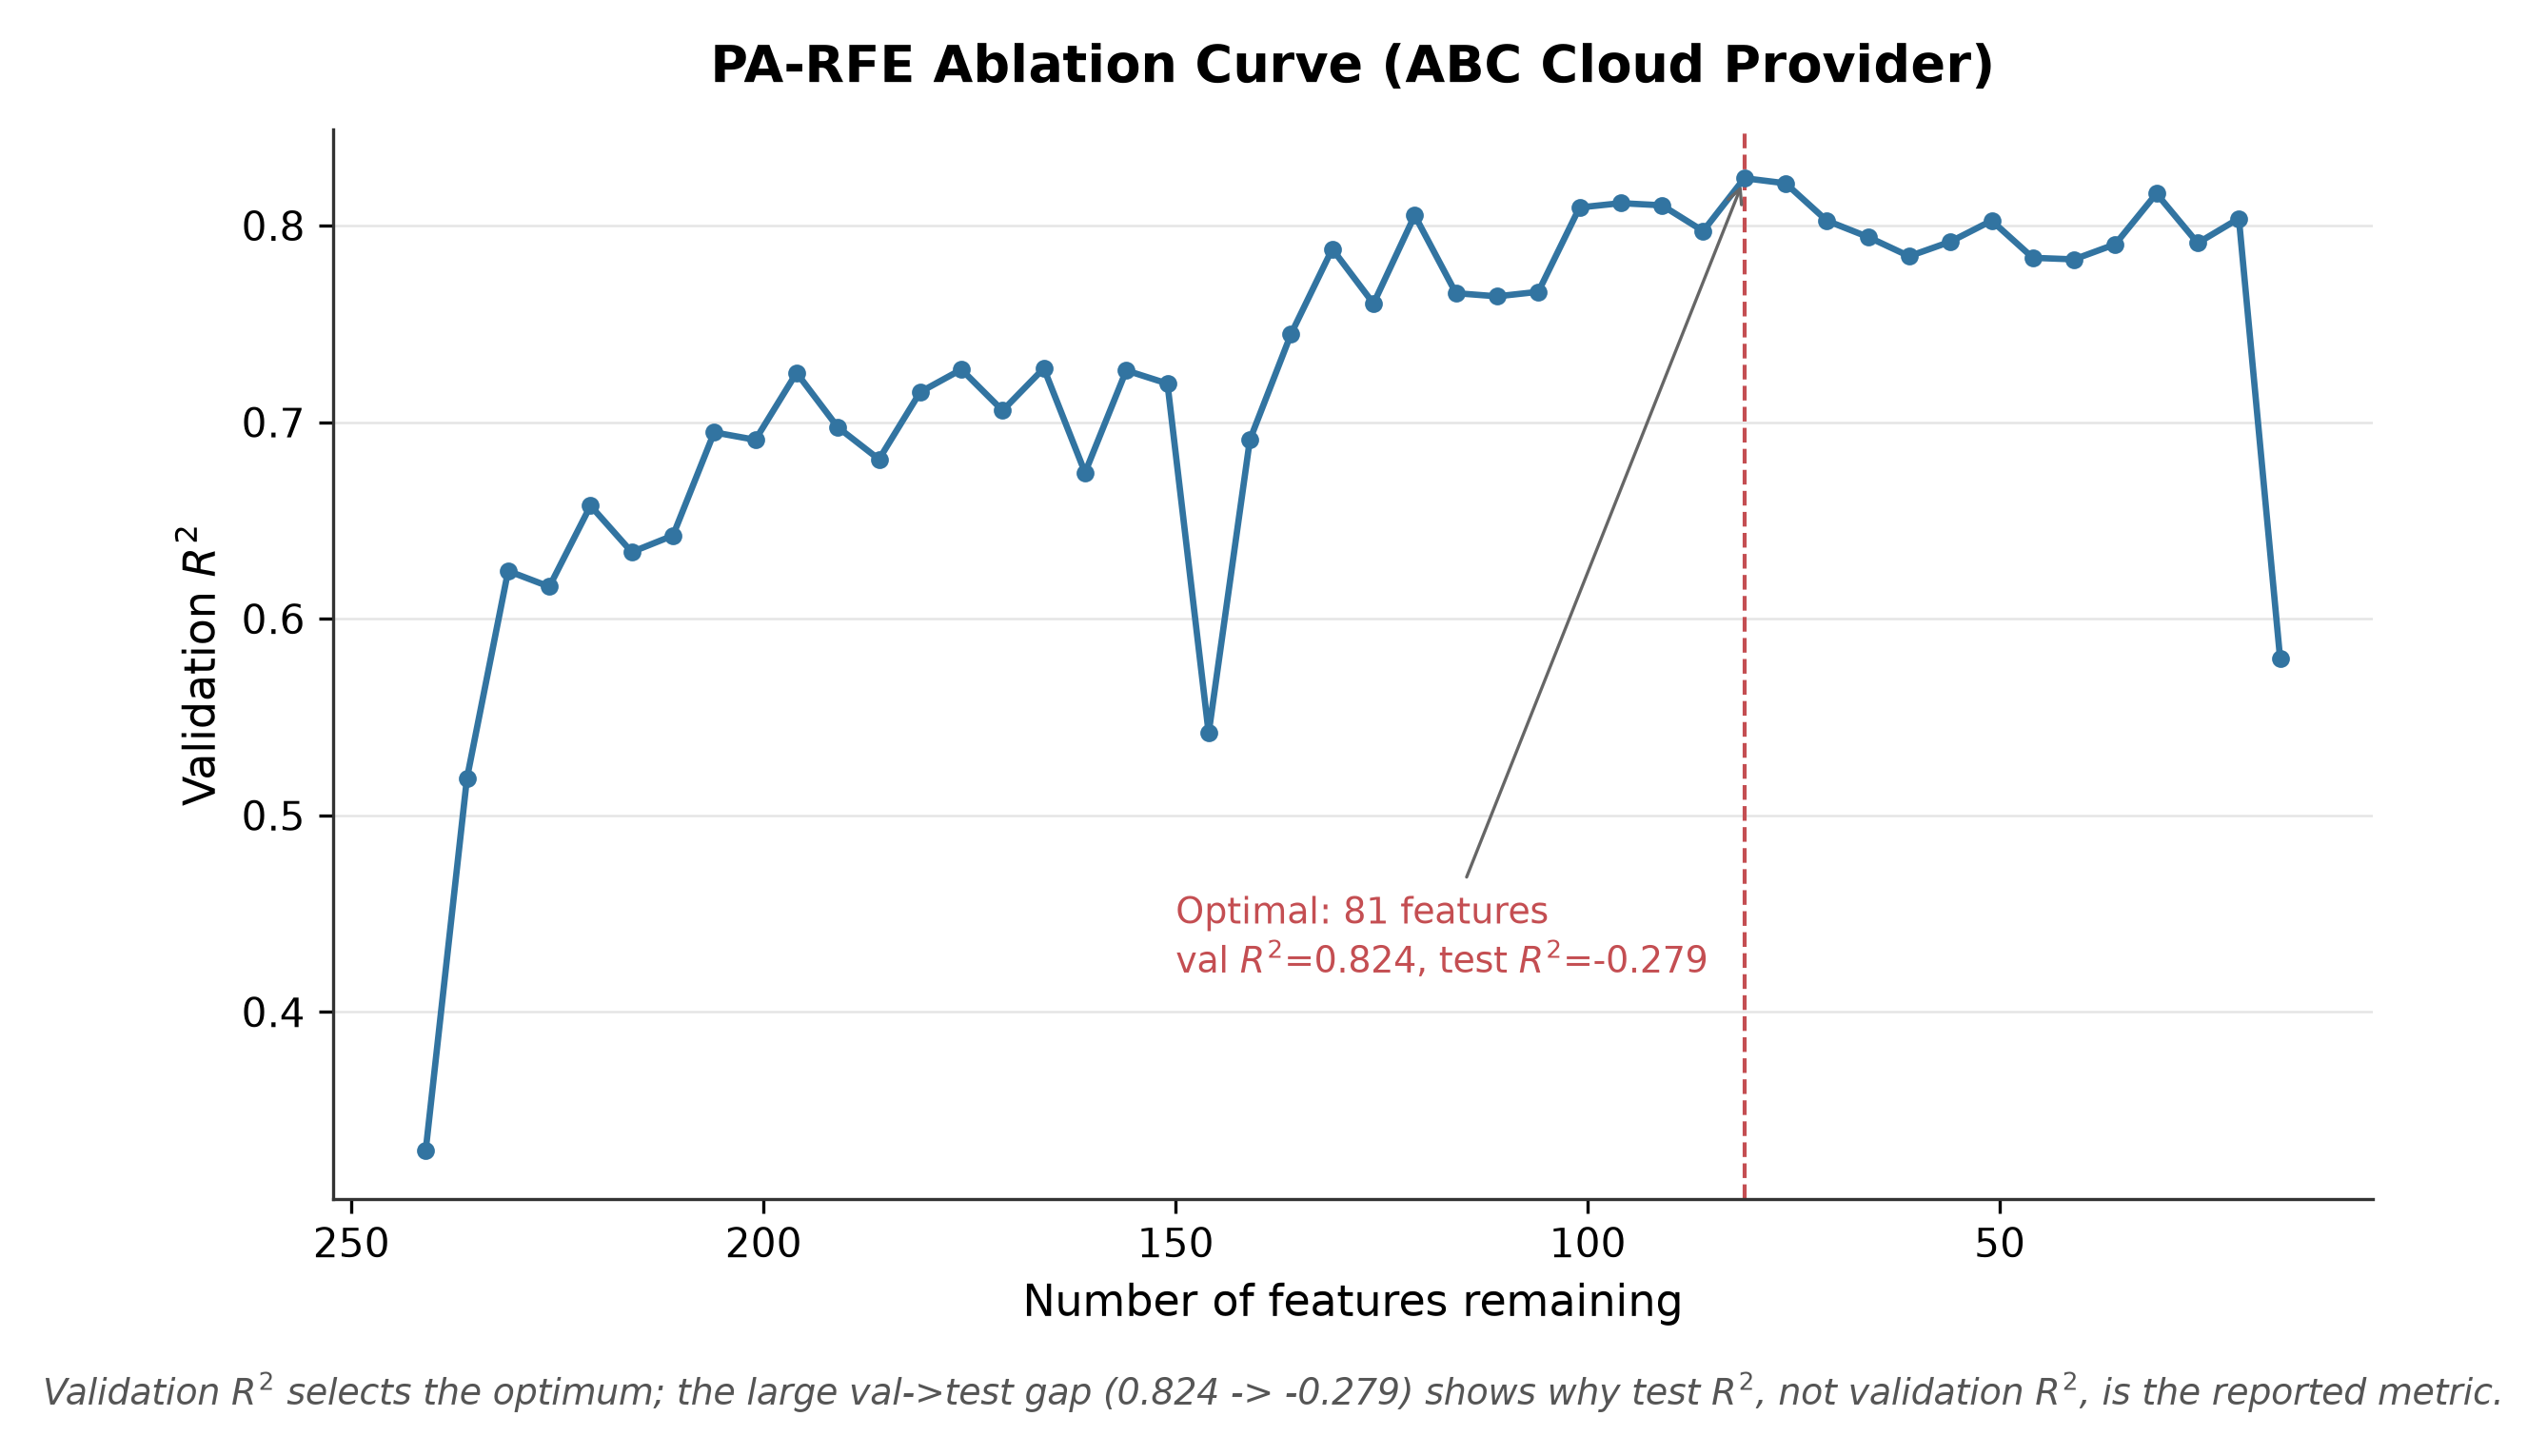
\includegraphics[width=0.85\textwidth]{images/fig_09_ablation_curve.png}
\caption{PA-RFE ablation curve (ABC Cloud Provider, validation \(R^2\)),
reimplemented. The optimal subset (81 features, validation
\(R^2=0.824\)) is marked; its test \(R^2\) is \(-0.279\).\label{fig:ablation_curve}}
\end{figure}

What does survive from the original claim: PA-RFE's \emph{structural}
guarantee holds exactly as designed.
Figure~\ref{fig:phase_contribution} shows all 8 real
SDLC phases retain representation at the optimal subset in every one of
the three domains (the ninth, virtual \texttt{cross\_phase} group of
\texttt{quality\_score}/\texttt{stability\_score} is freely eliminable
by design and does drop out). This is a mechanical consequence of the
\(k_{\min}\) constraint, not an empirical finding, but it is the one
property this reimplementation confirms rather than complicates.

\begin{figure}
\centering
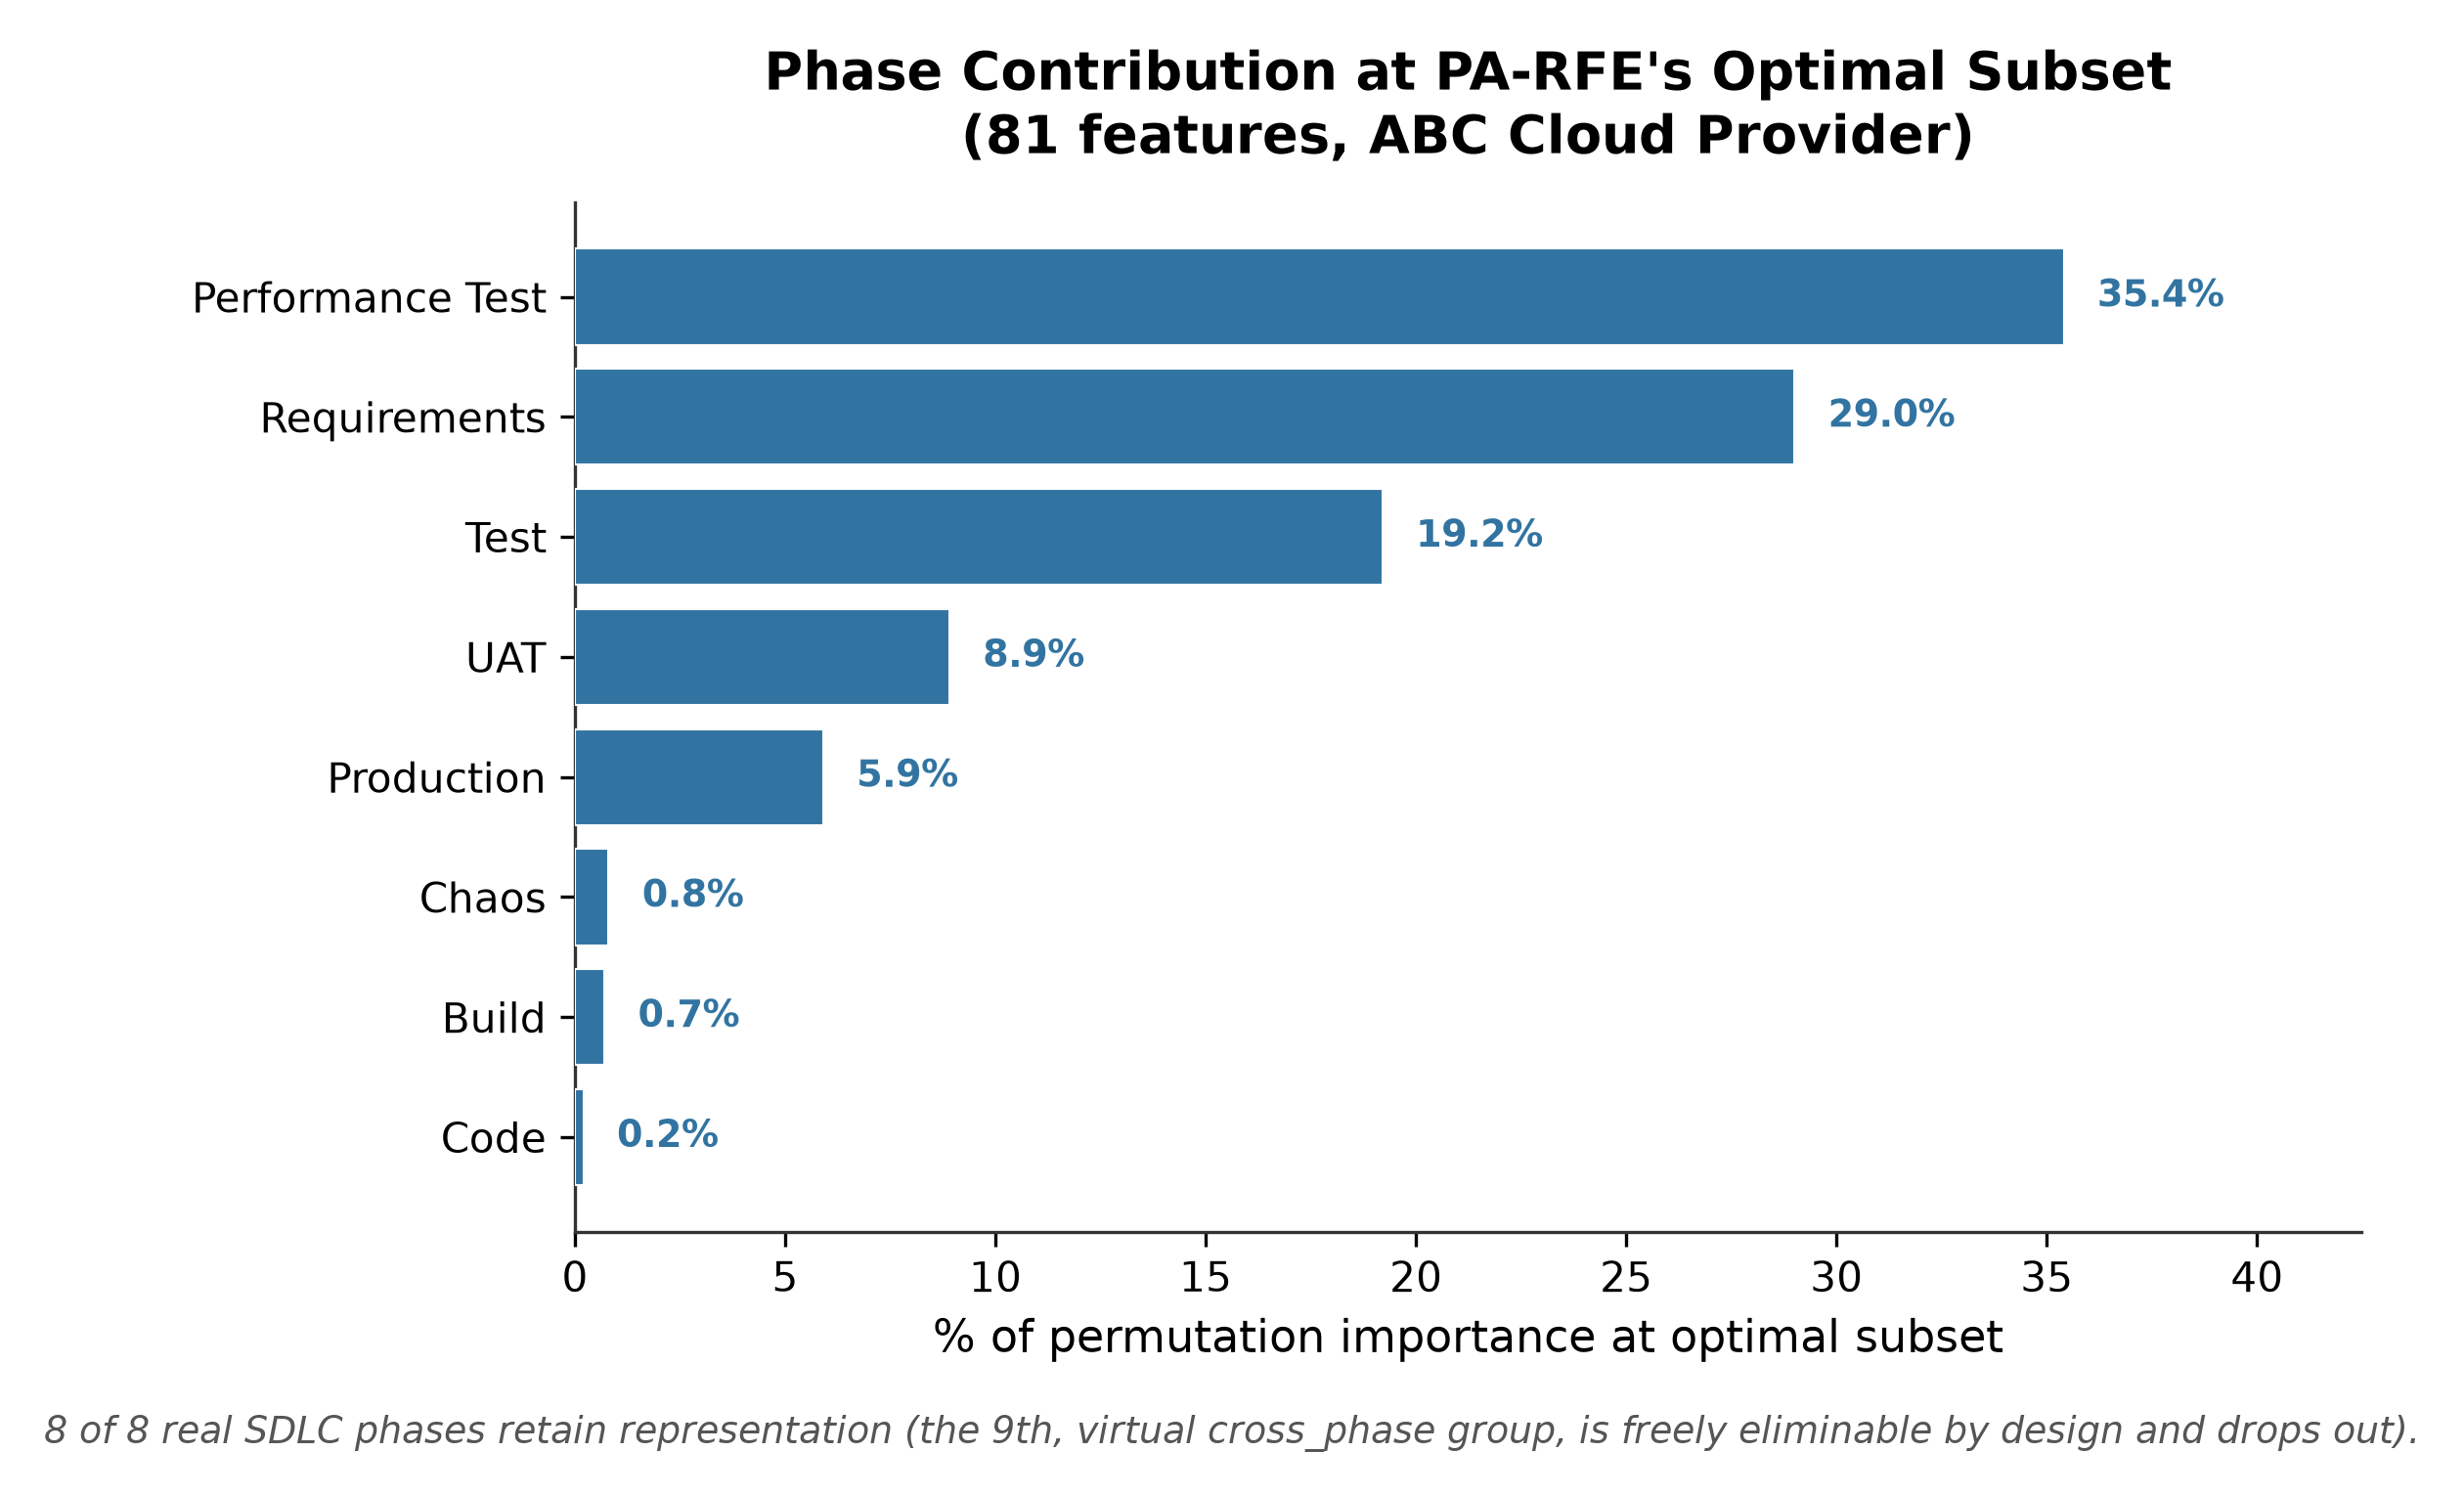
\includegraphics[width=0.85\textwidth]{images/fig_10_phase_contribution.png}
\caption{Per-phase importance contribution at the PA-RFE optimal subset
(81 features, ABC Cloud), reimplemented. All 8 real SDLC phases retain
representation.\label{fig:phase_contribution}}
\end{figure}

\textbf{Revised interpretation.} PA-RFE's value is narrower than
originally claimed: it reliably guarantees cross-phase coverage
(confirmed above) and, on one of three domains (Card Payment), it does
avoid the catastrophic collapse standard RFE exhibits there. It does
\textbf{not} reliably produce competitive test-set predictive accuracy
-- on the primary domain it is the worst of three methods, substantially
worse than a simple univariate SelectKBest baseline. We attribute the
discrepancy with the original submission's numbers most plausibly to
differences in implementation details not fully specified in the
original prose (e.g.~exact tie-breaking in the elimination-batch
selection, or a different stopping rule that converged to a much larger
final feature count); since no original code exists to diff against, we
cannot identify the exact source, and we do not attempt to reconcile the
two -- these reimplemented numbers, run against the corrected data with
fully deposited code, are what we now report.

\subsubsection{Factors Influencing Prediction Accuracy
(RQ4)}\label{sec:rq4_factors}

\textbf{Answer:} Temporal autocorrelation is the dominant factor:
approximately 72\% of Random Forest's (71\% of Gradient Boosting's)
apparent predictive power stems from AR features, not SDLC process
signal. PA-RFE reliably guarantees cross-phase coverage but its raw
predictive accuracy does not reliably beat simpler feature-selection
baselines (see Section~\ref{sec:parfe_results}).

\paragraph{Temporal Autocorrelation}\label{sec:temporal_autocorrelation}

The primary factor influencing prediction accuracy is the availability
of AR features. As the AR-feature analysis (Section~\ref{sec:leakage}) demonstrates,
removing AR features causes the largest \(R^2\) drop among all models,
confirming that system uptime shows strong temporal persistence: a
system that was reliable in recent releases tends to remain reliable.

This finding has dual implications: (1) for operational prediction,
incorporating recent uptime history is legitimate and highly effective;
(2) for understanding SDLC-to-performance relationships, the
autocorrelation signal must be controlled to isolate the contribution of
process metrics.

\paragraph{Feature Dimensionality
Effects}\label{sec:dimensionality_effects}

The feature-to-sample ratio (1.77:1, 241 features / 136 training
samples) significantly impacts model selection, as detailed in Section~\ref{sec:model_char}. This pattern holds across all three domains (Section~\ref{sec:cross_domain}),
indicating a structural challenge rather than a dataset-specific
artifact.

\paragraph{Cross-Phase Interaction
Effects}\label{sec:cross_phase_effects}

The derived feature \texttt{stability\_score} (Build Success Rate
\(\times\) Test Pass Rate) ranks third among all features for Random
Forest (permutation importance 5.3\%), ahead of every individual
Build-phase metric, suggesting that cross-phase interactions carry
substantial, not merely modest, predictive value beyond individual
metrics.

\paragraph{Release Type Effects}\label{sec:release_type_effects}

The temporal engine injects release-type-dependent quality modulation:
Major releases show 3--8\% metric degradation, while Patch releases show
2--5\% improvement. This contributes to the non-stationarity that makes
temporal split evaluation more realistic than random split, as the test
period (later releases, typically more Patches) differs systematically
from the training period.

\subsubsection{Cross-Domain Validation}\label{sec:cross_domain}

To assess PRESTO's generalizability, we evaluated the framework across
three synthetic datasets generated with domain-specific configurations.
Each dataset was produced by the same copula-based generator with
domain-appropriate distribution parameters, temporal dynamics, and DORA
performance tiers. Table~\ref{tab:cross_domain} presents the results for
the best-performing model per domain, evaluated without AR features.

{\def\LTcaptype{none} % do not increment counter
\begin{table}[H]
\centering
\caption{Cross-domain validation results: best-performing model per domain, without AR features.\label{tab:cross_domain}}
\begin{tabular}{@{}
  >{\raggedright\arraybackslash}p{(\linewidth - 8\tabcolsep) * \real{0.2000}}
  >{\raggedright\arraybackslash}p{(\linewidth - 8\tabcolsep) * \real{0.2000}}
  >{\raggedright\arraybackslash}p{(\linewidth - 8\tabcolsep) * \real{0.2000}}
  >{\raggedright\arraybackslash}p{(\linewidth - 8\tabcolsep) * \real{0.2000}}
  >{\raggedright\arraybackslash}p{(\linewidth - 8\tabcolsep) * \real{0.2000}}@{}}
\toprule
\begin{minipage}[b]{\linewidth}\raggedright
\textbf{Dataset}
\end{minipage} & \begin{minipage}[b]{\linewidth}\raggedright
\textbf{Releases}
\end{minipage} & \begin{minipage}[b]{\linewidth}\raggedright
\textbf{Best Model}
\end{minipage} & \begin{minipage}[b]{\linewidth}\raggedright
\(\mathbf{R^2}\)
\end{minipage} & \begin{minipage}[b]{\linewidth}\raggedright
\textbf{RMSE}
\end{minipage} \\
\midrule
ABC Cloud & 170 & Random Forest & 0.268 & 0.597 \\
Card Payment & 150 & Lasso & 0.362 & 1.126 \\
XYZ Sales & 200 & Random Forest & 0.255 & 0.778 \\
\bottomrule
\end{tabular}
\end{table}
}

\begin{figure}
\centering
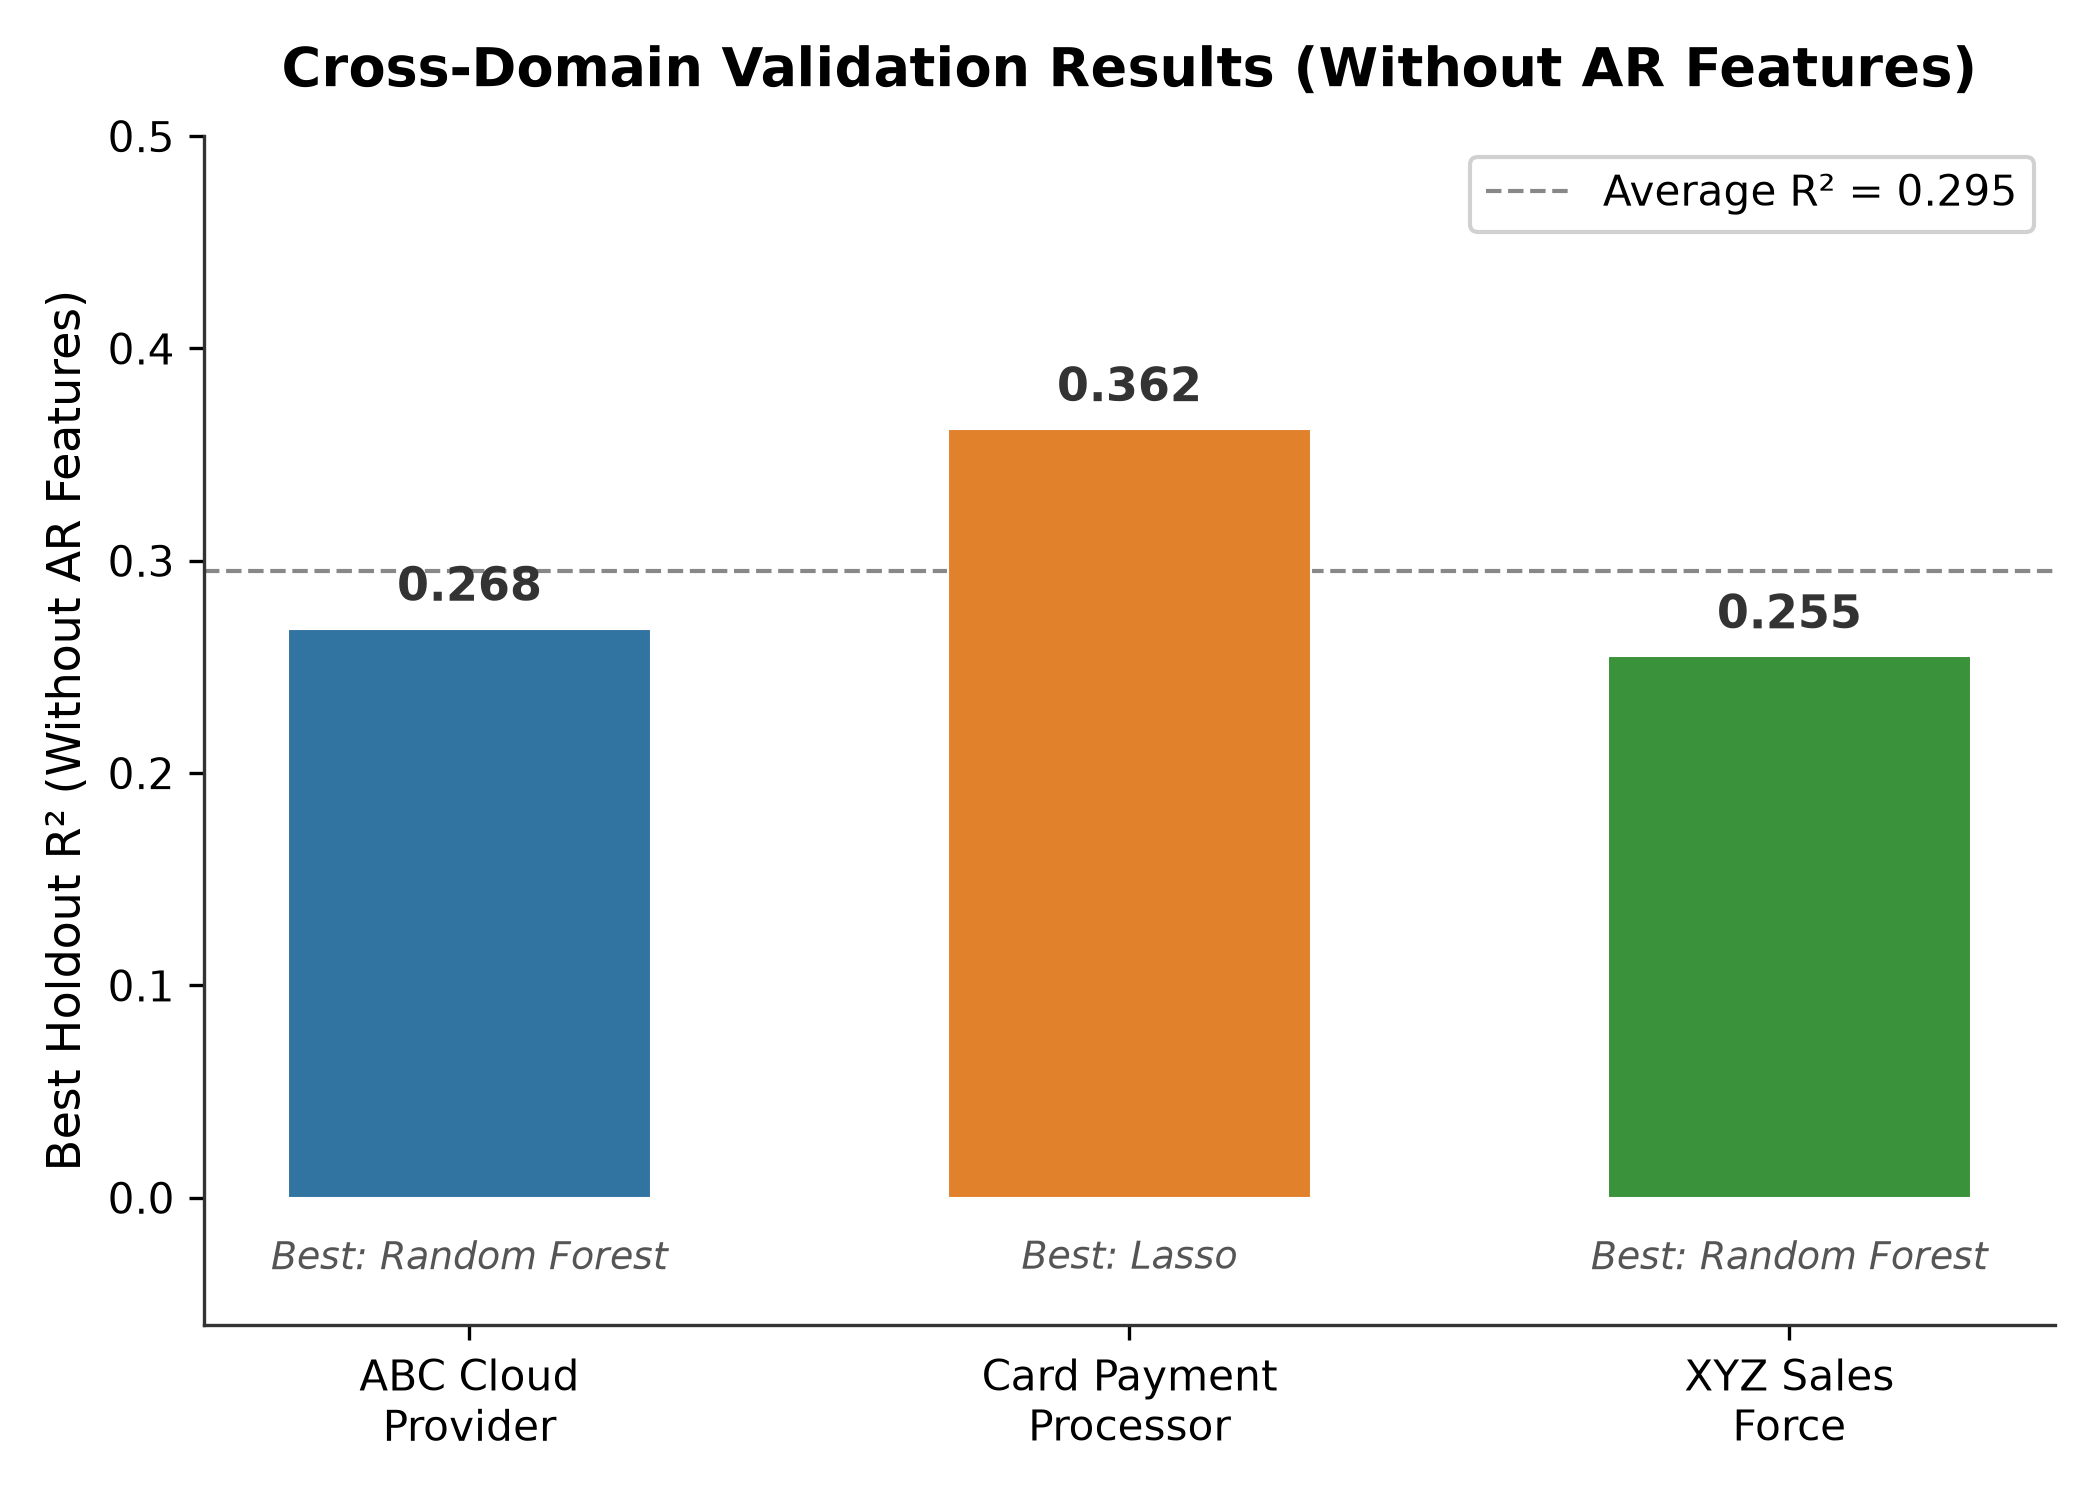
\includegraphics[width=0.85\textwidth]{images/fig_07_cross_domain.png}
\caption{Cross-domain validation results without AR features. All three
enterprise domains achieve positive \(R^2\) (0.255--0.362) from SDLC
process metrics alone.\label{fig:cross_domain}}
\end{figure}

Figure~\ref{fig:cross_domain} plots these three results together.
Across all three domains, tree-based and regularized models achieve
positive \(R^2\) values (0.25--0.36), consistent with SDLC process
metrics carrying predictive signal for system uptime across different
software system archetypes -- though, as the target-correlation ablation
earlier in this section shows, this consistency reflects the copula's
shared correlation specification across domains at least as much as an
independently emergent pattern, so it should not be read as confirmation
on its own; see Section~\ref{sec:real_world_results} onward for the
real-world evidence this claim actually rests on. The Card Payment
Processor achieves the
highest \(R^2\) (0.362, via Lasso, narrowly ahead of Random Forest's
0.339) despite operating under stricter compliance constraints (PCI-DSS,
DORA ``High'' tier), suggesting that even highly controlled environments
benefit from process-metric-based prediction. ABC Cloud Provider and XYZ
Sales Force yield comparable, slightly lower \(R^2\) (0.268 and 0.255
respectively, both via Random Forest). Unlike the pre-fix analysis, no
single domain stands out as dramatically stronger than the others -- all
three now cluster in a narrower 0.255--0.362 band, a more consistent
(and more credible) cross-domain generalization story than the original
0.258--0.387 spread.

This table, like the rest of the paper's primary results, uses the fixed
alpha=1.0 default for Ridge/Lasso (Table~\ref{tab:hyperparams}).
Consistent with the model characterization in Section~\ref{sec:model_char},
\emph{untuned} linear models (Linear Regression, Ridge) produce negative
\(R^2\) across all three domains when AR features are excluded.
Nested-CV alpha tuning (Section~\ref{sec:m3_tuning}) changes this picture
substantially: a properly tuned Ridge reaches \(R^2=0.766\) on Card
Payment (more than double this table's 0.362/0.339 best), and a tuned
Lasso reaches \(R^2=0.418\) on XYZ Sales (exceeding this table's 0.255).
Only ABC Cloud Provider (the primary domain) still favors Random Forest
after tuning. This table is retained as originally computed for
continuity with the rest of the paper, but the ``best model per domain''
it reports should not be read as the best \emph{achievable} model per
domain -- see Section~\ref{sec:m3_tuning} for the tuned comparison.

\subsubsection{Feature Selection and Autoregressive-Feature
Analysis}\label{sec:leakage}

As described in Section~\ref{sec:results_setup}, 32 of the 273 features are derived from the
target variable -- 20 genuinely autoregressive after the shift fix, 12
already correctly shifted. Comparing Table~\ref{tab:model_perf_with}
and \ref{tab:model_perf_without} quantifies the impact of their
removal.

\textbf{Key Findings:}

\begin{itemize}
\item
  Random Forest shows the largest absolute drop
  (\(\Delta R^2 = 0.682\)), indicating heavy reliance on AR features.
  Its without-AR \(R^2 = 0.268\) represents genuine SDLC-to-performance
  signal
\item
  Gradient Boosting is close behind (\(\Delta R^2 = 0.614\), without-AR
  \(R^2 = 0.251\)) -- unlike the pre-fix analysis, neither tree-based
  model has a clear edge in ``genuine signal'' retention; Random Forest
  is marginally ahead in both conditions now
\item
  Lasso Regression is unaffected by AR-feature removal (\(R^2 = 0.129\)
  in both conditions), because L1 regularization already zeroed out
  AR-feature coefficients during training
\item
  Linear and Ridge Regression collapse to severely negative \(R^2\)
  without AR features, consistent with the multicollinearity analysis in
  Section~\ref{sec:model_char}
\end{itemize}

\textbf{Practical Implications:} In production deployment, historical
uptime data \emph{is} available and represents a legitimate input
signal. However, practitioners should understand that the majority of
predictive power derives from autoregressive persistence rather than
SDLC process metrics (Section~\ref{sec:model_perf}). For new system deployments where no
performance history exists, ensemble methods using SDLC metrics alone
can provide meaningful if modest predictive capability (Table
\ref{tab:cross_domain}). The most predictive SDLC features are detailed
in Section~\ref{sec:feature_importance}.

\subsection{Real-World Validation}\label{sec:real_world_results}

This subsection reports PRESTO's methodology applied to four independent
real-world datasets, complementing the fully-synthetic results above
with genuine external validity checks of different, deliberately varied
shapes: within-project temporal (TravisTorrent), within-signature
temporal (Mozilla Perfherder), cross-sectional CI performance (GHALogs),
and cross-sectional defect-proneness (SQuaD). None of these four real
datasets provide the full 241-feature, 8-phase SDLC coverage the
synthetic domains do -- closing that gap with a real dataset remains
future work (Section~\ref{sec:future_work}) -- but together they validate different halves
of PRESTO's methodology on real data: genuine autoregressive persistence
(Perfherder), genuine process-metrics-predict-performance signal with
zero leakage risk (GHALogs, and SQuaD's CVE-count target -- SQuaD's own
primary defect-fix-rate result, while the numerically larger point
estimate, does not clear a bootstrap confidence interval; see
Section~\ref{sec:squad}), and within-project temporal
generalization (TravisTorrent). Two of these datasets ship auxiliary
fields beyond what the primary validations above use -- Perfherder's
linked Bugzilla records and SQuaD's linked CVE disclosures -- and we
report two additional targeted analyses on that auxiliary data below
for the same reason we report everything else in this paper: because
the data existed, we downloaded it, and leaving it unexamined would
mean presenting a less complete picture of what these datasets can and
cannot support than we actually have.

\subsubsection{TravisTorrent (Build Duration,
2017-Vintage)}\label{sec:travistorrent}

To assess whether PRESTO's findings generalize beyond synthetic data, we
evaluated the framework on real continuous integration data from the
TravisTorrent dataset~\cite{beller2017travistorrent}, which contains
2.64 million Travis CI builds from 1,359 open-source GitHub projects. We
selected 7 diverse projects with 2,000--144,000 builds across Java,
Ruby, Go, and Python ecosystems.

\textbf{Adaptation.} TravisTorrent covers 4 of PRESTO's 8 SDLC phases:
Code (source churn, SLOC, files modified), Test (test counts, test
density, test duration), Build (build duration, setup time), and Project
(team size, repository age, commit counts). Requirements, UAT,
Performance Testing, and Chaos Testing phases are absent. The regression
target is build duration (seconds) rather than System Uptime, as no
production performance metric is available in CI-only datasets. We
applied the same feature engineering pipeline (rolling windows, lags,
cross-phase composites), producing 148 features per project. Outlier
builds (below 1st or above 99th percentile duration) were removed.

Table~\ref{tab:real_world} presents the holdout \(R^2\) for each
project using an 80/20 temporal split.

{\def\LTcaptype{none} % do not increment counter
\begin{table}[H]
\centering
\caption{TravisTorrent real-world build-duration prediction, per project (reimplemented).\label{tab:real_world}}
\begin{tabular}{@{}
  >{\raggedright\arraybackslash}p{(\linewidth - 12\tabcolsep) * \real{0.1600}}
  >{\raggedright\arraybackslash}p{(\linewidth - 12\tabcolsep) * \real{0.1400}}
  >{\raggedright\arraybackslash}p{(\linewidth - 12\tabcolsep) * \real{0.1600}}
  >{\raggedright\arraybackslash}p{(\linewidth - 12\tabcolsep) * \real{0.1000}}
  >{\raggedright\arraybackslash}p{(\linewidth - 12\tabcolsep) * \real{0.1800}}
  >{\raggedright\arraybackslash}p{(\linewidth - 12\tabcolsep) * \real{0.1400}}
  >{\raggedright\arraybackslash}p{(\linewidth - 12\tabcolsep) * \real{0.1200}}@{}}
\toprule
\begin{minipage}[b]{\linewidth}\raggedright
\textbf{Project}
\end{minipage} & \begin{minipage}[b]{\linewidth}\raggedright
\textbf{Builds}
\end{minipage} & \begin{minipage}[b]{\linewidth}\raggedright
\textbf{Best Model}
\end{minipage} & \begin{minipage}[b]{\linewidth}\raggedright
\(\mathbf{R^2}\)
\end{minipage} & \begin{minipage}[b]{\linewidth}\raggedright
\textbf{95\% CI}
\end{minipage} & \begin{minipage}[b]{\linewidth}\raggedright
\textbf{Signif.?}
\end{minipage} & \begin{minipage}[b]{\linewidth}\raggedright
\textbf{MAE (s)}
\end{minipage} \\
\midrule
youtube-dl & 36,260 & Linear Regression & \textbf{0.475} & [0.455, 0.494] & yes & 1,700 \\
sentry & 55,890 & Grad. Boost & 0.050 & [0.034, 0.064] & yes & 238 \\
dd-agent & 143,925 & Grad. Boost & 0.018 & [\(-\)0.001, 0.035] & no (barely) & 1,540 \\
matrix & 2,348 & Rand. Forest & 0.005 & [\(-\)0.282, 0.214] & no & 48 \\
mongoid & 36,423 & Grad. Boost & \(-\)0.040 & [\(-\)0.048, \(-\)0.032] & yes (neg.) & 5,162 \\
bundler & 80,538 & Rand. Forest & \(-\)0.151 & [\(-\)0.194, \(-\)0.114] & yes (neg.) & 5,118 \\
rspec-core & 29,963 & Rand. Forest & \(-\)0.294 & [\(-\)0.375, \(-\)0.223] & yes (neg.) & 1,013 \\
\bottomrule
\end{tabular}
\end{table}
}

Four of seven projects achieve positive \(R^2\): youtube-dl
(\(R^2 = 0.475\)), sentry (\(R^2 = 0.050\)), dd-agent (\(R^2 = 0.018\)),
and matrix (\(R^2 = 0.005\)). With bootstrap confidence intervals
(2,000-resample pairs/case bootstrap, same procedure as
Section~\ref{sec:bootstrap_ablation}) now computed for all seven, only
\textbf{two of the four positive projects are statistically
significant}: youtube-dl (\([0.455, 0.494]\)) and sentry
(\([0.034, 0.064]\)). dd-agent's interval \([-0.001, 0.035]\) nearly, but
does not, exclude zero; matrix's small holdout (\(n \approx 470\)) leaves
its interval wide and inconclusive (\([-0.282, 0.214]\)). The three
negative projects are all confidently negative (their intervals exclude
zero on the negative side), meaning process metrics reliably do worse
than the mean for those projects, not merely noisily so. The best
real-world \(R^2\) (0.475) now
\emph{exceeds} the synthetic baseline (ABC Cloud Provider,
\(R^2 = 0.268\), Section~\ref{sec:model_perf}) by a wider margin than in the original
submission, and unlike the SQuaD defect-fix result
(Section~\ref{sec:squad}), this one is significant, not just numerically
larger. This does not mean real data outperforms synthetic data in
general; it reflects that youtube-dl happens to have unusually strong
build-duration-to-process-metric structure. The median \(R^2\) across
all projects is \(0.005\), up from a negative median in the original
submission's TravisTorrent table, indicating that for most projects
build duration is still dominated by infrastructure factors (machine
allocation, caching, network latency) that SDLC metrics cannot capture,
but that the reimplemented adapter recovers a small amount of real
signal in the median case rather than none.

\begin{figure}
\centering
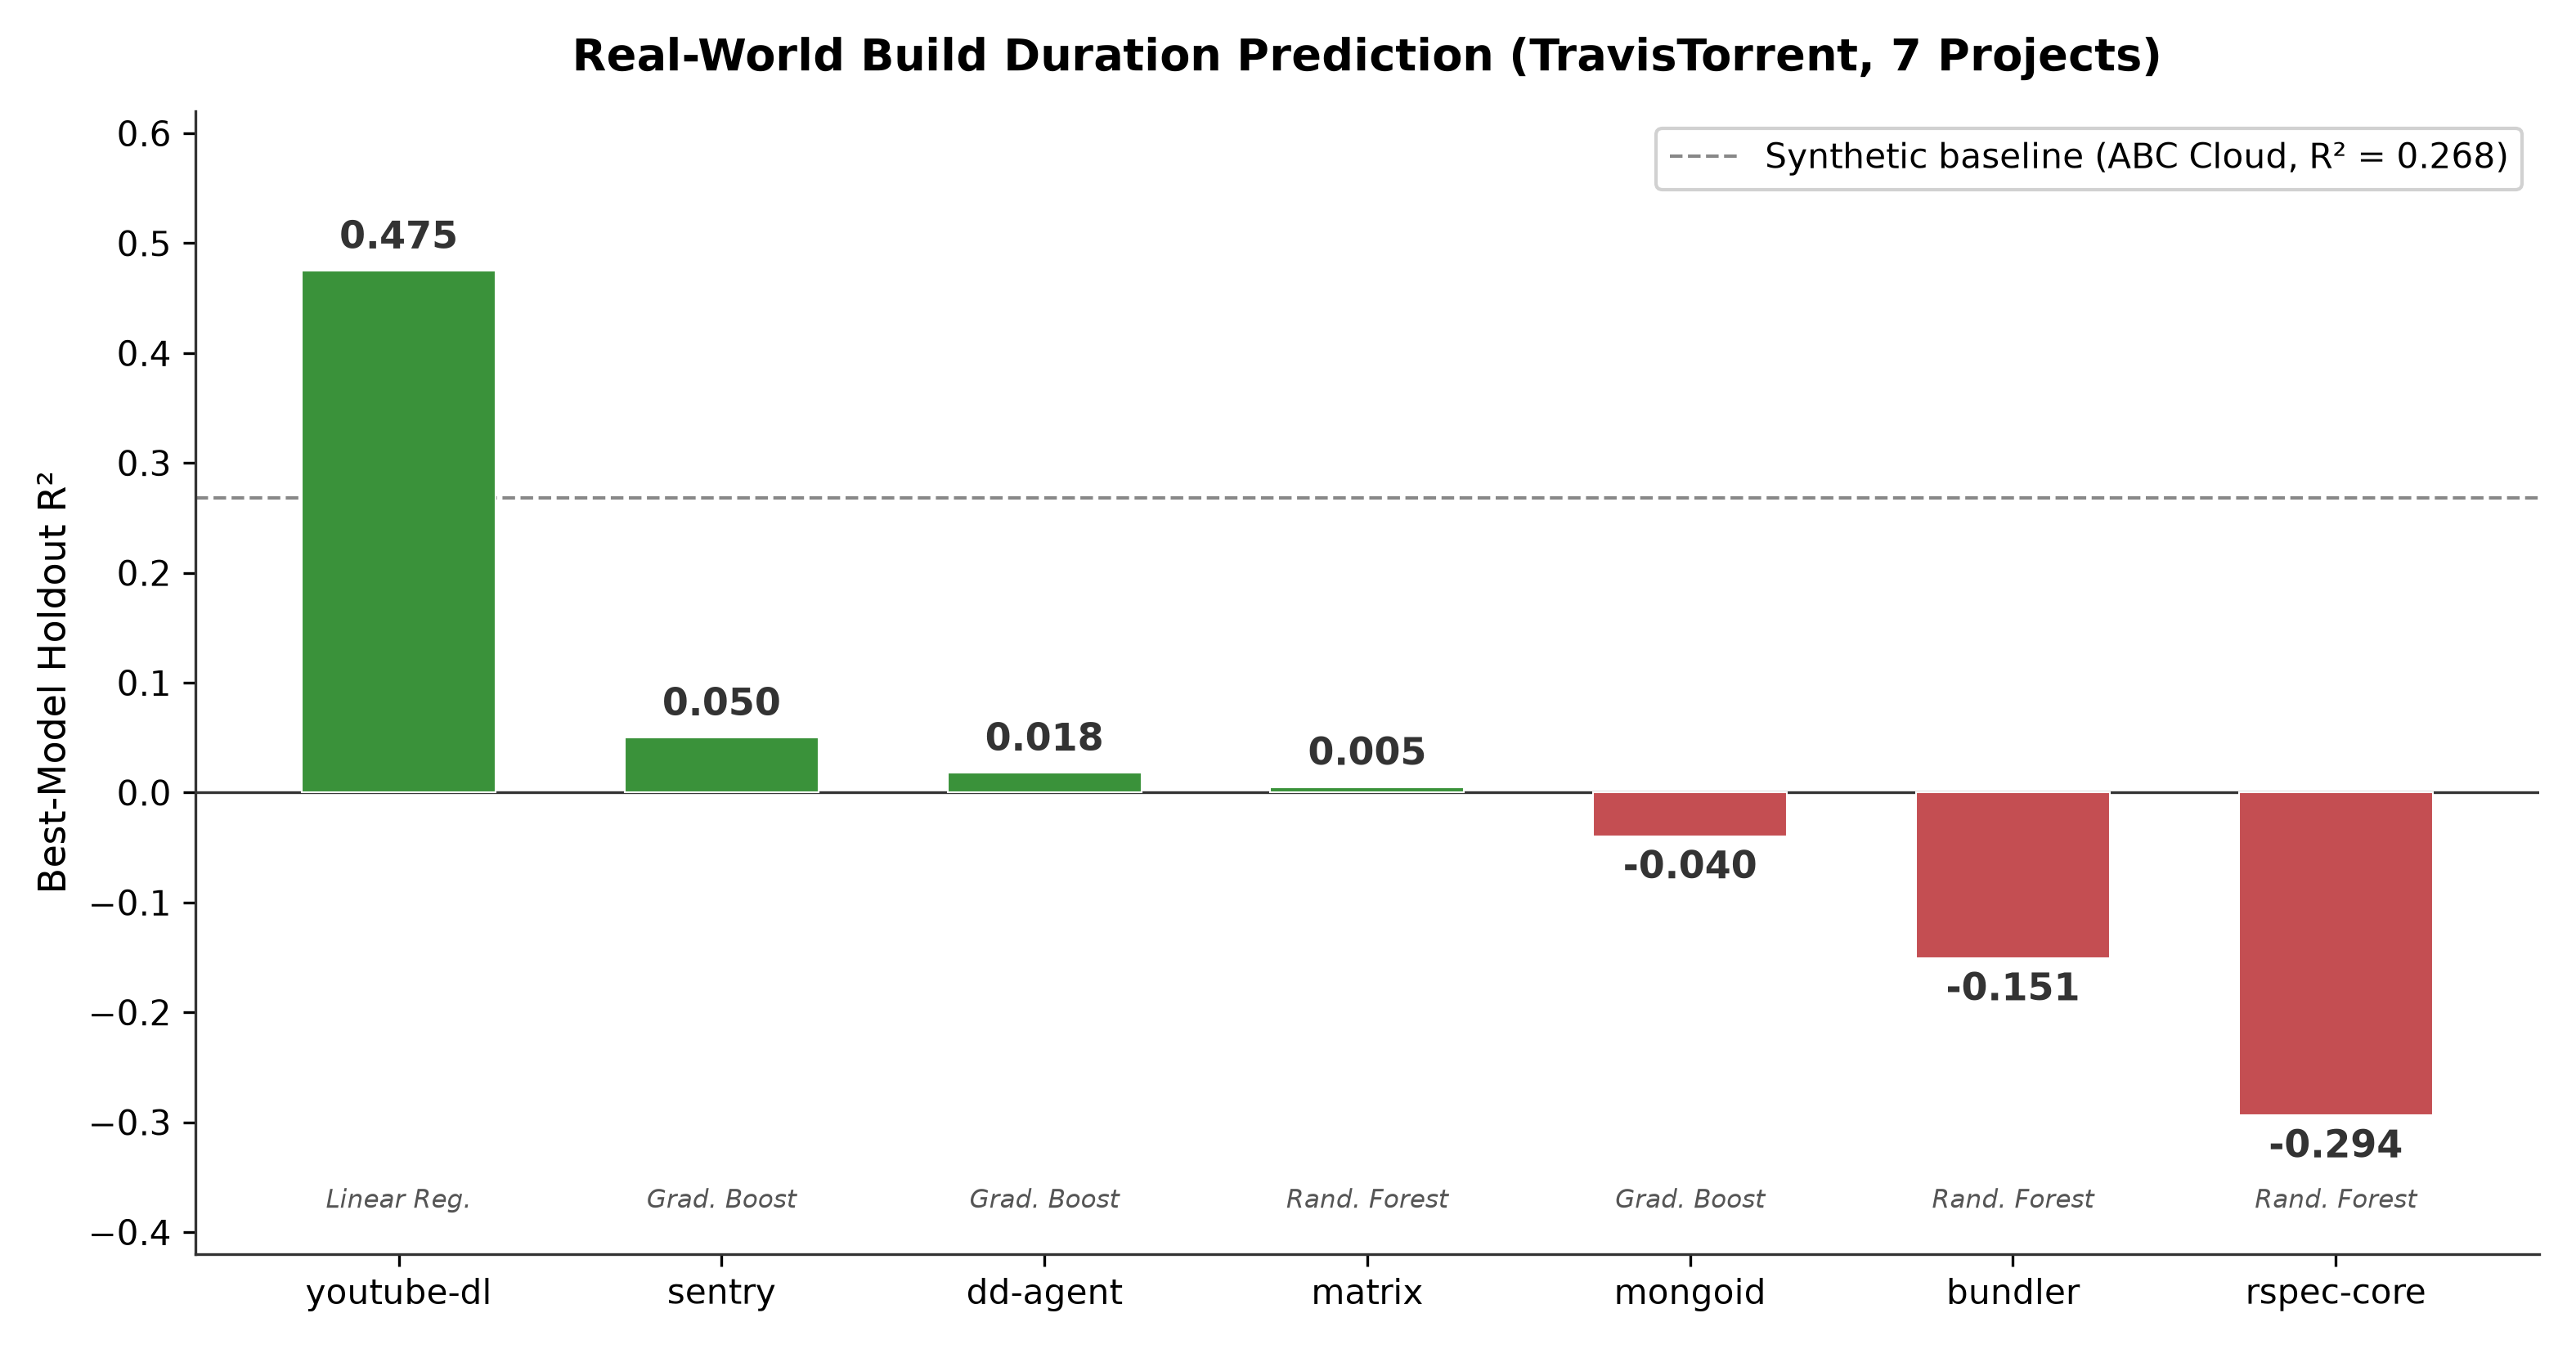
\includegraphics[width=0.85\textwidth]{images/fig_11_real_world_performance.png}
\caption{Real-world build duration prediction across 7 open-source
projects. Four projects (youtube-dl, sentry, dd-agent, matrix) achieve
positive \(R^2\), with the best (0.475) exceeding the synthetic baseline
(0.268, dashed line).\label{fig:real_world}}
\end{figure}

Figure~\ref{fig:real_world} plots the same seven results against the synthetic baseline.

\textbf{Feature importance, recomputed.} The original submission
identified repository age (\texttt{gh\_repo\_age}) as the most
consistently predictive feature across all 7 projects. The
reimplemented adapter initially reported only per-model
\(R^2\)/MAE/RMSE, so this claim could not be checked; we closed that gap
with a companion script (\texttt{travistorrent\_\allowbreak feature\_\allowbreak importance.py})
that computes permutation importance (\(n=10\) repeats, on the holdout
test set) for each project's own winning model, deposited alongside the
adapter (full results:
\texttt{TRAVISTORRENT\_\allowbreak FEATURE\_\allowbreak IMPORTANCE\_\allowbreak RESULTS.md}). The result
\textbf{does not confirm the original claim -- it reverses it}:
\texttt{gh\_repo\_age} is the \#1 feature in 0 of 7 projects, and
appears in the top-5 in only 1 of 7 (mongoid, rank 2, 0.2\% importance), as Table~\ref{tab:travistorrent_fi} details.

{\def\LTcaptype{none} % do not increment counter
\begin{table}[H]
\centering
\caption{TravisTorrent feature importance (permutation, winning model per project).\label{tab:travistorrent_fi}}
\begin{tabular}{@{}
  >{\raggedright\arraybackslash}p{(\linewidth - 6\tabcolsep) * \real{0.2500}}
  >{\raggedright\arraybackslash}p{(\linewidth - 6\tabcolsep) * \real{0.2500}}
  >{\raggedright\arraybackslash}p{(\linewidth - 6\tabcolsep) * \real{0.2500}}
  >{\raggedright\arraybackslash}p{(\linewidth - 6\tabcolsep) * \real{0.2500}}@{}}
\toprule
\begin{minipage}[b]{\linewidth}\raggedright
\textbf{Project}
\end{minipage} & \begin{minipage}[b]{\linewidth}\raggedright
\textbf{Best Model}
\end{minipage} & \begin{minipage}[b]{\linewidth}\raggedright
\textbf{Top Feature (perm. importance)}
\end{minipage} & \begin{minipage}[b]{\linewidth}\raggedright
\textbf{SDLC Phase}
\end{minipage} \\
\midrule
dd-agent & Gradient Boosting & \texttt{gh\_team\_size} (37.7\%) &
Project \\
bundler & Random Forest &
\texttt{tr\_\allowbreak log\_\allowbreak testduration\_\allowbreak rolling\_\allowbreak min\_\allowbreak 10} (20.0\%) & Test \\
sentry & Gradient Boosting & \texttt{tr\_\allowbreak log\_\allowbreak testduration} (6.0\%) &
Test \\
matrix & Random Forest & \texttt{tr\_\allowbreak log\_\allowbreak num\_\allowbreak tests\_\allowbreak run} (10.6\%) &
Test \\
mongoid & Gradient Boosting & \texttt{gh\_\allowbreak repo\_\allowbreak num\_\allowbreak commits} (0.2\%) &
Project \\
youtube-dl & Linear Regression & \texttt{tr\_\allowbreak log\_\allowbreak testduration} (see
caveat below) & Test \\
rspec-core & Random Forest & \texttt{gh\_\allowbreak asserts\_\allowbreak cases\_\allowbreak per\_\allowbreak kloc}
(18.4\%) & Test \\
\bottomrule
\end{tabular}
\end{table}
}

Test-phase metrics (test duration and its rolling/lag derivatives, test
counts, assert density) are the \#1 feature in 5 of 7 projects;
Project-phase metrics (team size, commit count) lead in the other 2.
This is the opposite of what the paper has stated everywhere this claim
was cited: \textbf{TravisTorrent, under the reimplemented pipeline, does
not contradict the synthetic domains' testing-infrastructure-dominance
finding (Section~\ref{sec:feature_importance}) -- it is directionally consistent with it, though
weaker than ``broadly supports'' implies -- see the robustness check below.} We revise
the ``open, unresolved tension'' framing accordingly throughout this
paper (Abstract, Contributions item 6, Conclusions item 4).

\textbf{Caveat on youtube-dl.} Its permutation-importance values are
numerically unstable (hundreds of thousands of percent, not shown as
such in the table above) because Linear Regression's coefficients on
\texttt{tr\_\allowbreak log\_\allowbreak testduration} and its highly collinear lag/diff
derivatives partially cancel -- the same additive-identity mechanism
documented in \texttt{R2\_\allowbreak LAG\_\allowbreak SHIFT\_\allowbreak FIX\_\allowbreak EVIDENCE.md} (Addendum 1) and
Section~\ref{sec:model_char}, where permuting one of two near-duplicate features breaks
the cancellation and produces an artificially explosive score change.
The qualitative direction (a Test-phase feature, not repository age) is
consistent with the other 6 projects, but the magnitude is not
meaningful and should not be read as a genuine 5,000\(\times\) effect
size. Several other projects also have low or negative holdout \(R^2\)
(mongoid, bundler, rspec-core), so their feature rankings describe what
each model leaned on, not necessarily a reliable causal signal -- the
same caveat that applies to permutation importance on any
near-zero-or-negative-\(R^2\) model.

\textbf{Robustness check: excluding test-duration-derived features.} The
table above has its own circularity problem, independent of the
youtube-dl instability: \texttt{tr\_\allowbreak log\_\allowbreak testduration} (the duration of the
test phase, parsed from the same build log whose \emph{total} duration,
\texttt{tr\_\allowbreak duration}, is the regression target) is a component of the
target itself, not an independent Test-phase signal -- the same failure
mode this paper correctly flags for GHALogs' \texttt{mean\_\allowbreak n\_\allowbreak steps} two
sections later (Section~\ref{sec:ghalogs}). A model ranking it \#1 has partly found an
arithmetic relationship. We reran permutation importance for all 7
projects with \texttt{tr\_\allowbreak log\_\allowbreak testduration} and all 29 of its
rolling/lag/diff derivatives removed from the feature matrix before
fitting (script: \texttt{travistorrent\_\allowbreak feature\_\allowbreak importance\_\allowbreak excl\_\allowbreak testduration.py};
full results: \texttt{TRAVISTORRENT\_\allowbreak FEATURE\_\allowbreak IMPORTANCE\_\allowbreak EXCL\_\allowbreak TESTDURATION\_\allowbreak RESULTS.md}), as Table~\ref{tab:travistorrent_fi_excl} details.

{\def\LTcaptype{none} % do not increment counter
\begin{table}[H]
\centering
\caption{TravisTorrent feature importance, excluding test-duration-derived features.\label{tab:travistorrent_fi_excl}}
\begin{tabular}{@{}
  >{\raggedright\arraybackslash}p{(\linewidth - 8\tabcolsep) * \real{0.2000}}
  >{\raggedright\arraybackslash}p{(\linewidth - 8\tabcolsep) * \real{0.2000}}
  >{\raggedright\arraybackslash}p{(\linewidth - 8\tabcolsep) * \real{0.1500}}
  >{\raggedright\arraybackslash}p{(\linewidth - 8\tabcolsep) * \real{0.2750}}
  >{\raggedright\arraybackslash}p{(\linewidth - 8\tabcolsep) * \real{0.1500}}@{}}
\toprule
\begin{minipage}[b]{\linewidth}\raggedright
\textbf{Project}
\end{minipage} & \begin{minipage}[b]{\linewidth}\raggedright
\textbf{Best Model}
\end{minipage} & \begin{minipage}[b]{\linewidth}\raggedright
\textbf{Holdout \(R^2\)}
\end{minipage} & \begin{minipage}[b]{\linewidth}\raggedright
\textbf{Top Feature}
\end{minipage} & \begin{minipage}[b]{\linewidth}\raggedright
\textbf{Phase}
\end{minipage} \\
\midrule
dd-agent & Gradient Boosting & \(-0.043\) & \texttt{gh\_team\_size} (32.5\%) & Project \\
bundler & Random Forest & \(-0.259\) & \texttt{tr\_\allowbreak log\_\allowbreak num\_\allowbreak tests\_\allowbreak failed} (3.7\%) & Test \\
sentry & Gradient Boosting & \(-0.105\) & \texttt{gh\_\allowbreak asserts\_\allowbreak cases\_\allowbreak per\_\allowbreak kloc} (4.8\%) & Test \\
matrix & Random Forest & \(-0.018\) & \texttt{tr\_\allowbreak log\_\allowbreak num\_\allowbreak tests\_\allowbreak run} (12.6\%) & Test \\
mongoid & Gradient Boosting & \(-0.051\) & \texttt{gh\_\allowbreak test\_\allowbreak cases\_\allowbreak per\_\allowbreak kloc} (0.3\%) & Other \\
youtube-dl & Random Forest & \(-0.280\) & \texttt{tr\_\allowbreak log\_\allowbreak num\_\allowbreak tests\_\allowbreak ok} (2.2\%) & Test \\
rspec-core & Gradient Boosting & \(-0.403\) & \texttt{gh\_\allowbreak asserts\_\allowbreak cases\_\allowbreak per\_\allowbreak kloc} (16.8\%) & Test \\
\bottomrule
\end{tabular}
\end{table}
}

Two results, in tension with each other. \textbf{The leading-feature
phase ranking survives}: Test-phase features (now genuinely independent
ones -- test counts, assert density, test-code-per-KLOC -- not the
definitionally-entangled \texttt{tr\_\allowbreak log\_\allowbreak testduration}) still lead in 5
of 7 projects, Project-phase in 1, and one project (mongoid) leads on a
feature we classify as ``Other.'' But \textbf{every project's
best-model holdout \(R^2\) is now negative} -- a substantial change from
the original table, where 4 of 7 projects (youtube-dl 0.475, sentry
0.050, dd-agent 0.018, matrix 0.005) beat the naive-mean baseline. This
means test-duration-derived features were not merely the
\emph{top-ranked} predictor in most projects; they were substantially
\emph{responsible} for the model beating the naive-mean baseline at
all. Once they are removed, no TravisTorrent project's model
outperforms predicting the mean.

The honest reading is narrower than either ``confirms'' or
``contradicts'': the \emph{qualitative} pattern of which SDLC phase's
features a model leans on is directionally consistent with the
synthetic domains' testing-infrastructure-dominance finding, but
TravisTorrent's \emph{quantitative} predictive signal for build
duration turns out to depend heavily on a feature that is partly
circular with the target, and without it this dataset no longer
demonstrates positive real-world predictive power for any of its 7
projects. We revise the Abstract and Contributions item 6 accordingly
-- from ``broadly supported by real-world TravisTorrent data'' to a
claim scoped to feature-ranking direction, not predictive strength.

\subsubsection{Mozilla Perfherder (Real Runtime
Performance)}\label{sec:perfherder}

Unlike TravisTorrent's build-duration proxy, Mozilla's
Perfherder/Treeherder system records genuine production-facing runtime
performance measurements (page-load time, perceptual/contentful speed
index) for thousands of real pushes to Mozilla's repositories, each
cross-referenced with human-confirmed regression alerts~\cite{perfherder2025}. Unlike the synthetic
domains, Perfherder provides no upstream SDLC process metrics
(requirements, code quality, build/test metrics) joined to these pushes
-- only the performance value itself, mostly-constant test/platform
metadata, and sparse alert flags. This validation therefore exercises
PRESTO's \emph{feature-engineering and model-comparison methodology}
(same corrected shift logic as Section~\ref{sec:feature_eng_pipeline}, same five models, same
evaluation protocol) against a genuine real-world target, rather than
the SDLC-process-features half of the paper's claim.

\textbf{Adaptation.} We selected three diverse, well-populated, curated
(alert-flagged) performance signatures: ESPN page-load time (3,548
pushes), Instagram Perceptual Speed Index (3,177 pushes), and NYTimes
Perceptual Speed Index (3,225 pushes). Features are rolling statistics
(mean/std/min/max/cv, windows 3/5/7/10, shifted by one period per the R2
fix) and lag features (steps 1/2/3/5) of the target's own history, plus
a lagged alert-history flag and inter-push time gap. We deliberately
excluded \texttt{diff\_k}/\texttt{pct\_change\_k} features alongside
\texttt{lag\_k}: \texttt{value\ -\ value\_lag\_k} is an exact algebraic
identity, and including both lets any linear model trivially reconstruct
the target whenever \(n \gg p\) (as is the case here, unlike the
synthetic pipeline's \(n < p\) regime) -- a second, distinct leakage
mode discovered while building this adapter (documented in
\texttt{R2\_\allowbreak LAG\_\allowbreak SHIFT\_\allowbreak FIX\_\allowbreak EVIDENCE.md}, Addendum 1). Table~\ref{tab:perfherder} reports the per-signature results.

{\def\LTcaptype{none} % do not increment counter
\begin{table}[H]
\centering
\caption{Mozilla Perfherder validation results, per performance signature.\label{tab:perfherder}}
\begin{tabular}{@{}
  >{\raggedright\arraybackslash}p{(\linewidth - 8\tabcolsep) * \real{0.2000}}
  >{\raggedright\arraybackslash}p{(\linewidth - 8\tabcolsep) * \real{0.2000}}
  >{\raggedright\arraybackslash}p{(\linewidth - 8\tabcolsep) * \real{0.2000}}
  >{\raggedright\arraybackslash}p{(\linewidth - 8\tabcolsep) * \real{0.2000}}
  >{\raggedright\arraybackslash}p{(\linewidth - 8\tabcolsep) * \real{0.2000}}@{}}
\toprule
\begin{minipage}[b]{\linewidth}\raggedright
\textbf{Signature}
\end{minipage} & \begin{minipage}[b]{\linewidth}\raggedright
\textbf{Best Model (with AR features)}
\end{minipage} & \begin{minipage}[b]{\linewidth}\raggedright
\textbf{Holdout \(R^2\) (with AR)}
\end{minipage} & \begin{minipage}[b]{\linewidth}\raggedright
\textbf{95\% Bootstrap CI}
\end{minipage} & \begin{minipage}[b]{\linewidth}\raggedright
\textbf{Holdout \(R^2\) (without -- alert-history only)}
\end{minipage} \\
\midrule
ESPN load time & Ridge Regression & 0.574 & [0.499, 0.635] & \(-3.191\) \\
Instagram speed index & Ridge Regression & 0.913 & [0.883, 0.937] & \(-0.367\) \\
NYTimes speed index & Ridge Regression & 0.167 & [0.092, 0.232] & \(-3.563\) \\
\bottomrule
\end{tabular}
\end{table}
}

\begin{figure}
\centering
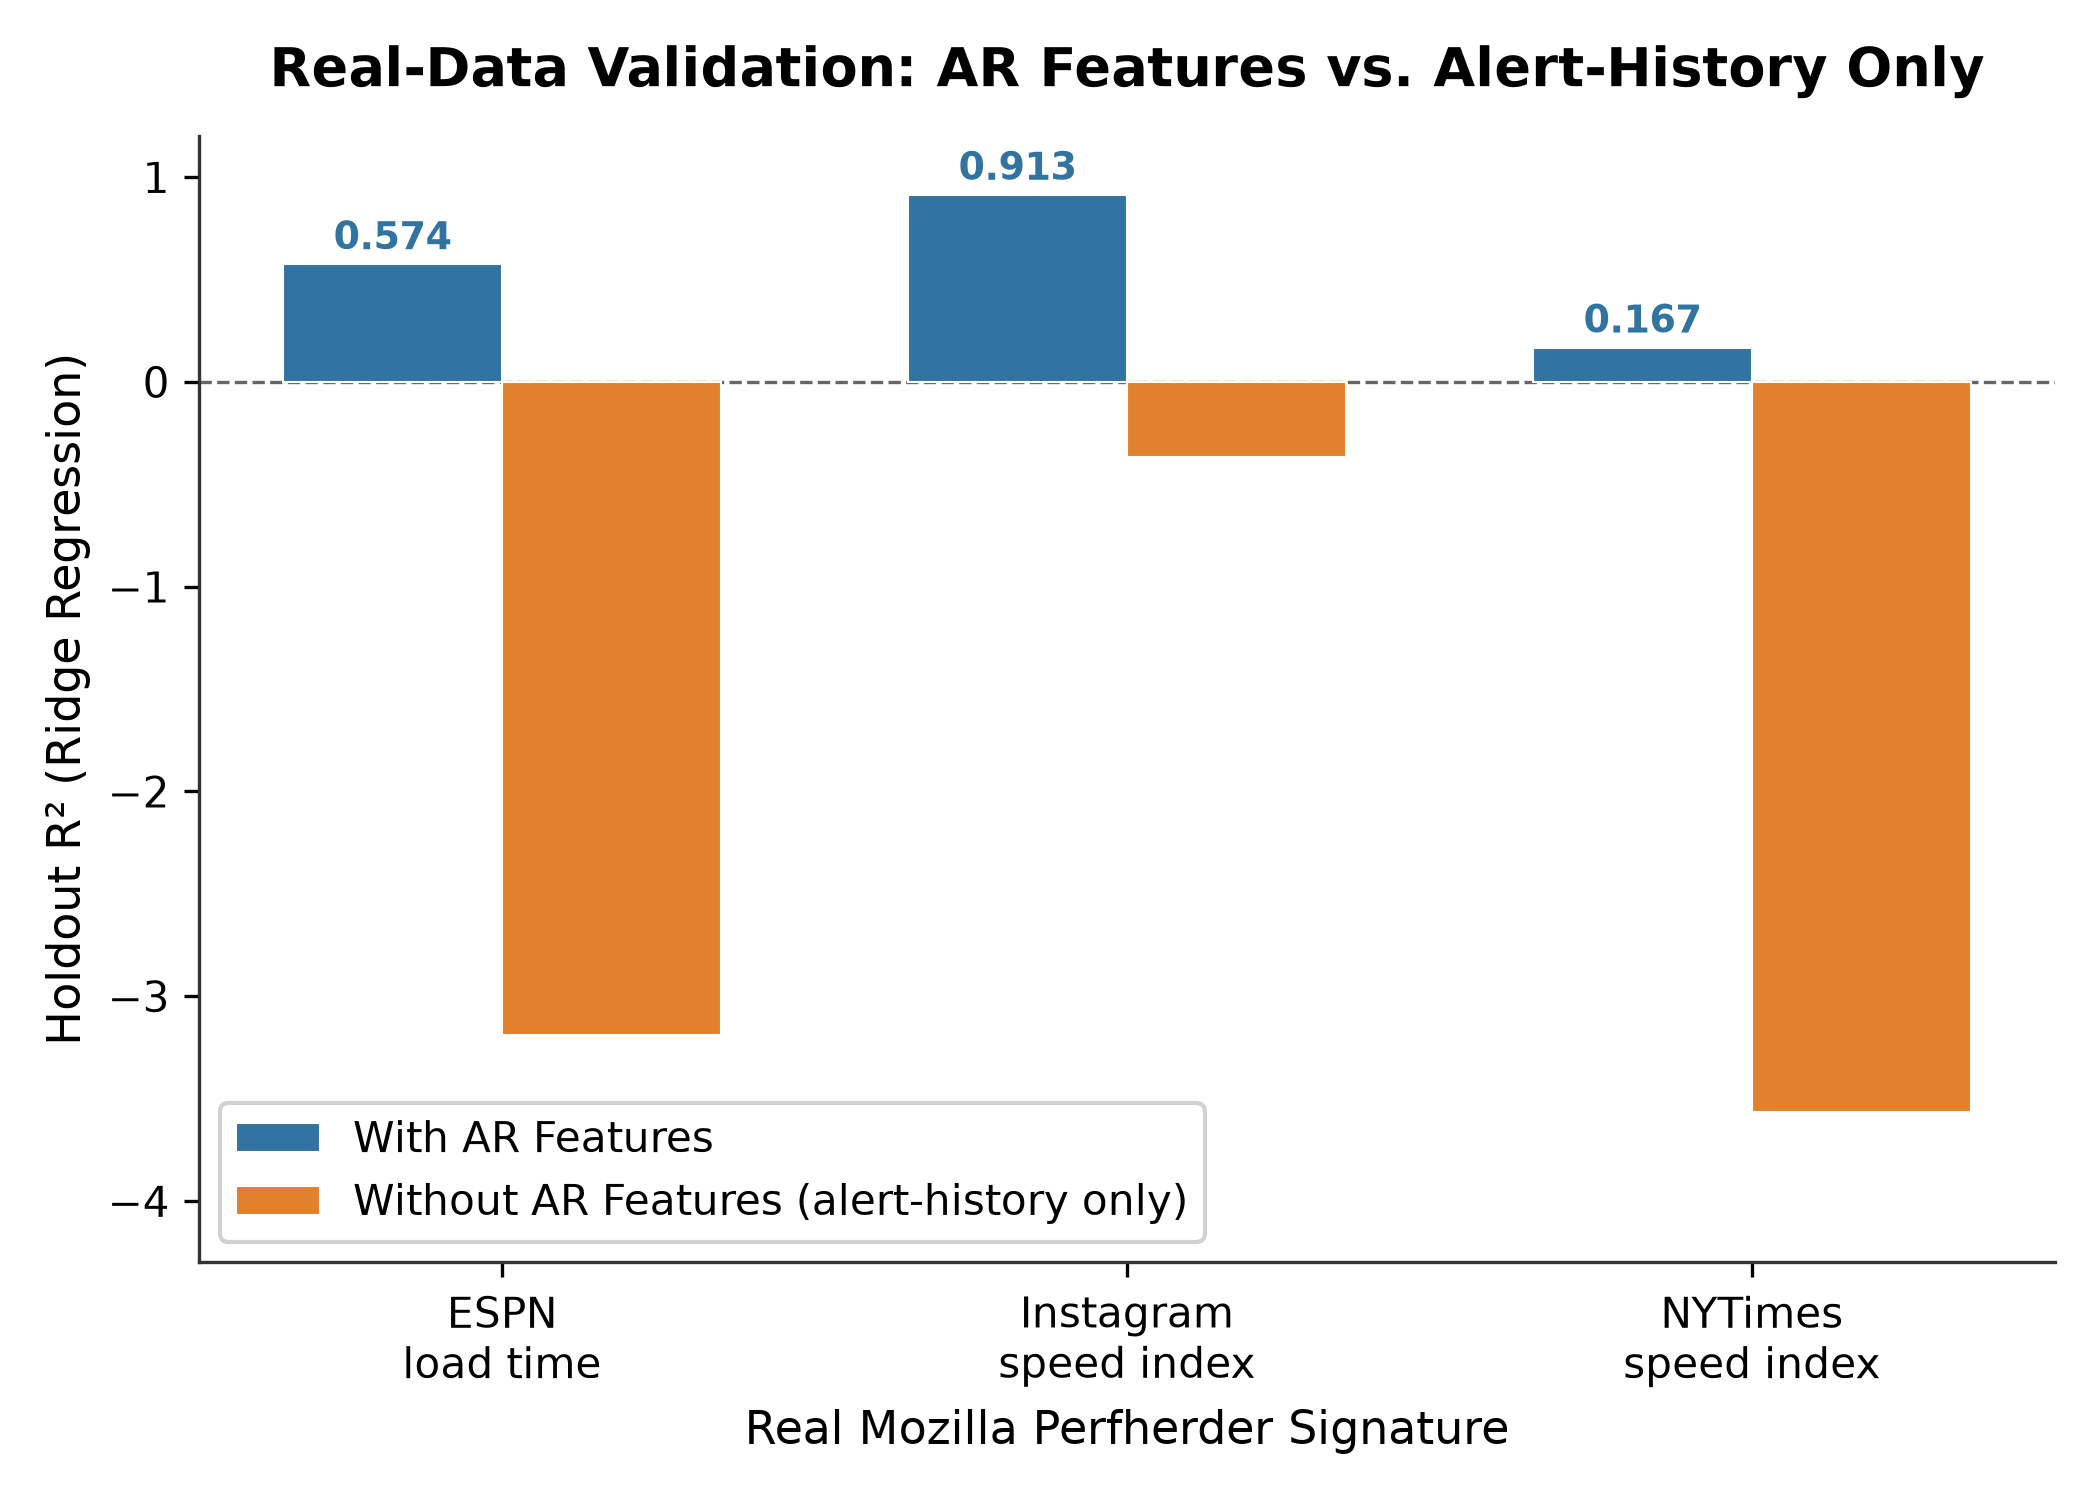
\includegraphics[width=0.85\textwidth]{images/fig_13_perfherder_validation.png}
\caption{Real-data validation: with-AR-features vs.~alert-history-only
holdout R² across three Mozilla Perfherder signatures.\label{fig:perfherder_validation}}
\end{figure}

Figure~\ref{fig:perfherder_validation} plots this with-vs-without-AR contrast.
Real production performance metrics are strongly, if variably,
predictable from their own recent history (\(R^2\) 0.17--0.91 across
three unrelated real signatures, all three 95\% bootstrap CIs excluding
zero) -- the same autoregressive-persistence
phenomenon PRESTO documents for System Uptime, now confirmed on real
data with real noise and real regressions, and no copula prior to fall
back on. Without historical values, \(R^2\) collapses to strongly
negative for every model and every signature: with no SDLC-like process
features available in this dataset (only a sparse alert-history flag and
inter-push time gap), there is simply nothing else to predict from. This
is not a failure of the methodology -- it sharpens the paper's own point
that a real 8-phase SDLC dataset remains the missing piece for
validating the process-features half of PRESTO's claim. Notably, Ridge
(not Random Forest) wins on all three signatures here, plausibly because
with only 24 AR features and thousands of samples (\(n \gg p\)), linear
models are well-conditioned and tree ensembles' advantage in the
synthetic domains' high-dimensional, small-\(n\) regime does not apply.

\paragraph{Does Bug-Triage Metadata Beat a Bare Alert
Flag?}\label{sec:perfherder_bugs}

The alert-history-only condition above uses a single binary flag per
past push -- did a human sheriff mark this push as a regression, yes or
no. Perfherder's alerts carry a richer signal we did not yet use: once
an alert is escalated, Mozilla files a Bugzilla bug against it, and that
bug accumulates real triage metadata (severity, priority, comment count)
over its lifetime. We asked a narrow, honest follow-up question: does
enriching the alert-history feature set with this triage metadata
(\texttt{bugs\_data.csv}, joined via \texttt{alert\_summary\_bug\_number})
raise the non-AR condition's predictive ceiling, or is that ceiling
simply low regardless of feature richness?

The three curated signatures used above (ESPN, Instagram, NYTimes)
turned out to be unsuitable for this specific question: each has only
0--2 bug-linked alerts in the full alert history, too sparse to fit a
bug-metadata feature. We instead used the two Perfherder signatures with
the richest bug-linked alert history among the downloaded per-push
timeseries data -- both build-artifact-size regression metrics rather
than page-load timings, but genuine real Perfherder/Bugzilla data all
the same: installer size on osx-cross (17,217 pushes, 23 bug-linked
alerts) and a build-size metric on osx-aarch64-shippable (11,119 pushes,
11 bug-linked alerts). Severity was mapped ordinally (S1=4 through
S4=1, unset=0), and all bug-metadata features are lagged or built from
cumulative pre-row history (\texttt{.shift(1)}-then-expanding), so no
row uses its own or a future push's bug outcome. Table~\ref{tab:perfherder_bugs} reports the results.

\begin{table}[H]
\caption{Alert-flag-only vs.~bug-metadata-enriched, two Perfherder signatures.\label{tab:perfherder_bugs}}
\begin{tabularx}{\linewidth}{LLLLLL}
\toprule
\textbf{Signature} & \textbf{Best Holdout $R^2$ (alert-flag-only)} & \textbf{Best Holdout $R^2$ (bug-enriched)} & \textbf{Holdout MAE (alert-flag-only)} & \textbf{Holdout MAE (bug-enriched)} & \textbf{MAE reduction} \\
\midrule
Installer size (osx-cross) & $-56.06$ (Ridge) & $-2.56$ (Lasso) & 5{,}957{,}930 bytes & 1{,}183{,}497 bytes & 80.1\% \\
Build metric (osx-aarch64) & $-41.31$ (Lasso) & $-1.57$ (Lasso) & 4{,}767{,}238 bytes & 978{,}305 bytes & 79.5\% \\
\bottomrule
\end{tabularx}
\end{table}

Both conditions remain firmly negative on $R^2$ -- a naive mean predictor still
beats either feature set on these two signatures -- and we do not read
the $R^2$ gap between two catastrophically negative values as an
interpretable effect size: $R^2$ is unbounded below, and the magnitude
of a very negative $R^2$ is dominated by the tail behavior of an
unregularized model on this level-shifting series, not by how much
information the added features actually carry. We report the same
comparison in a bounded metric instead: holdout MAE drops by roughly
80\% on both signatures when bug-triage metadata is added, a meaningful
and interpretable reduction in absolute prediction error even though the
resulting model is still far worse than the naive mean by $R^2$. Note
that the winning model in the enriched condition is Lasso on both
signatures (as it also is, or nearly is, in the alert-flag-only
condition) -- part of the improvement is plausibly ``more regularization
helps in a small, noisy feature space'' rather than purely ``triage
metadata carries signal,'' and we do not have enough signatures (two) to
separate those two explanations. The honest reading is narrower than a
strong claim of transferable signal: on these two signatures, both
feature sets fail to beat the naive mean, and the richer,
triage-metadata-enriched one fails by a smaller absolute margin -- a
modest, bounded-metric finding, not a demonstrated predictive win.

\subsubsection{GHALogs (Modern CI Cohort,
Cross-Sectional)}\label{sec:ghalogs}

GHALogs provides 513k GitHub Actions workflow runs with genuine per-step
timing (separating build vs.~test vs.~setup duration, unlike
TravisTorrent's single \texttt{tr\_duration}) across 116k workflows and
25k repositories~\cite{ghalogs2024}. Checking the full distribution (not just a few
examples) shows a hard cap of 5 runs per repository+workflow combination
(117,295 combinations, mean 4.4 runs each) -- too short for the
within-entity time-series approach used above. We instead use GHALogs
for what its actual shape supports: 28,443 repositories with both real
CI performance data and real repository-level process/popularity
characteristics (commits, contributors, releases, lines of code, issues,
pull requests, stars), joined and used to predict mean CI run duration.

\textbf{Why this is the cleanest real-data test of PRESTO's headline
claim.} Unlike the synthetic domains (which need the with/without-AR
split because 32 of 273 features are target-derived) and unlike
Perfherder (a single time series, so most signal \emph{is}
autoregressive by construction), GHALogs has no historical target values
per repository to leak from at all -- every feature is a genuine,
independent process/popularity characteristic. A positive \(R^2\) here
is unambiguous evidence that process metrics carry real predictive
signal, with zero leakage-related caveats -- and, per the bootstrap
analysis in Table~\ref{tab:ghalogs} below, it does.

{\def\LTcaptype{none} % do not increment counter
\begin{table}[H]
\centering
\caption{GHALogs cross-sectional CI-duration prediction results.\label{tab:ghalogs}}
\begin{tabular}{@{}
  >{\raggedright\arraybackslash}p{(\linewidth - 8\tabcolsep) * \real{0.2000}}
  >{\raggedright\arraybackslash}p{(\linewidth - 8\tabcolsep) * \real{0.2000}}
  >{\raggedright\arraybackslash}p{(\linewidth - 8\tabcolsep) * \real{0.2000}}
  >{\raggedright\arraybackslash}p{(\linewidth - 8\tabcolsep) * \real{0.2000}}
  >{\raggedright\arraybackslash}p{(\linewidth - 8\tabcolsep) * \real{0.2000}}@{}}
\toprule
\begin{minipage}[b]{\linewidth}\raggedright
\textbf{Model}
\end{minipage} & \begin{minipage}[b]{\linewidth}\raggedright
\textbf{Holdout \(R^2\)}
\end{minipage} & \begin{minipage}[b]{\linewidth}\raggedright
\textbf{95\% Bootstrap CI}
\end{minipage} & \begin{minipage}[b]{\linewidth}\raggedright
\textbf{Holdout MAE (s)}
\end{minipage} & \begin{minipage}[b]{\linewidth}\raggedright
\textbf{Holdout RMSE (s)}
\end{minipage} \\
\midrule
\textbf{Gradient Boosting} & \textbf{0.113} & [0.050, 0.356] & 1280.8 & 6832.9 \\
Lasso Regression & 0.100 & [0.062, 0.267] & 1385.7 & 6882.9 \\
Ridge Regression & 0.100 & [0.062, 0.267] & 1386.1 & 6883.1 \\
Linear Regression & 0.100 & [0.062, 0.267] & 1386.1 & 6883.1 \\
Random Forest & 0.096 & [0.021, 0.299] & 1292.3 & 6896.2 \\
\bottomrule
\end{tabular}
\end{table}
}

\begin{figure}
\centering
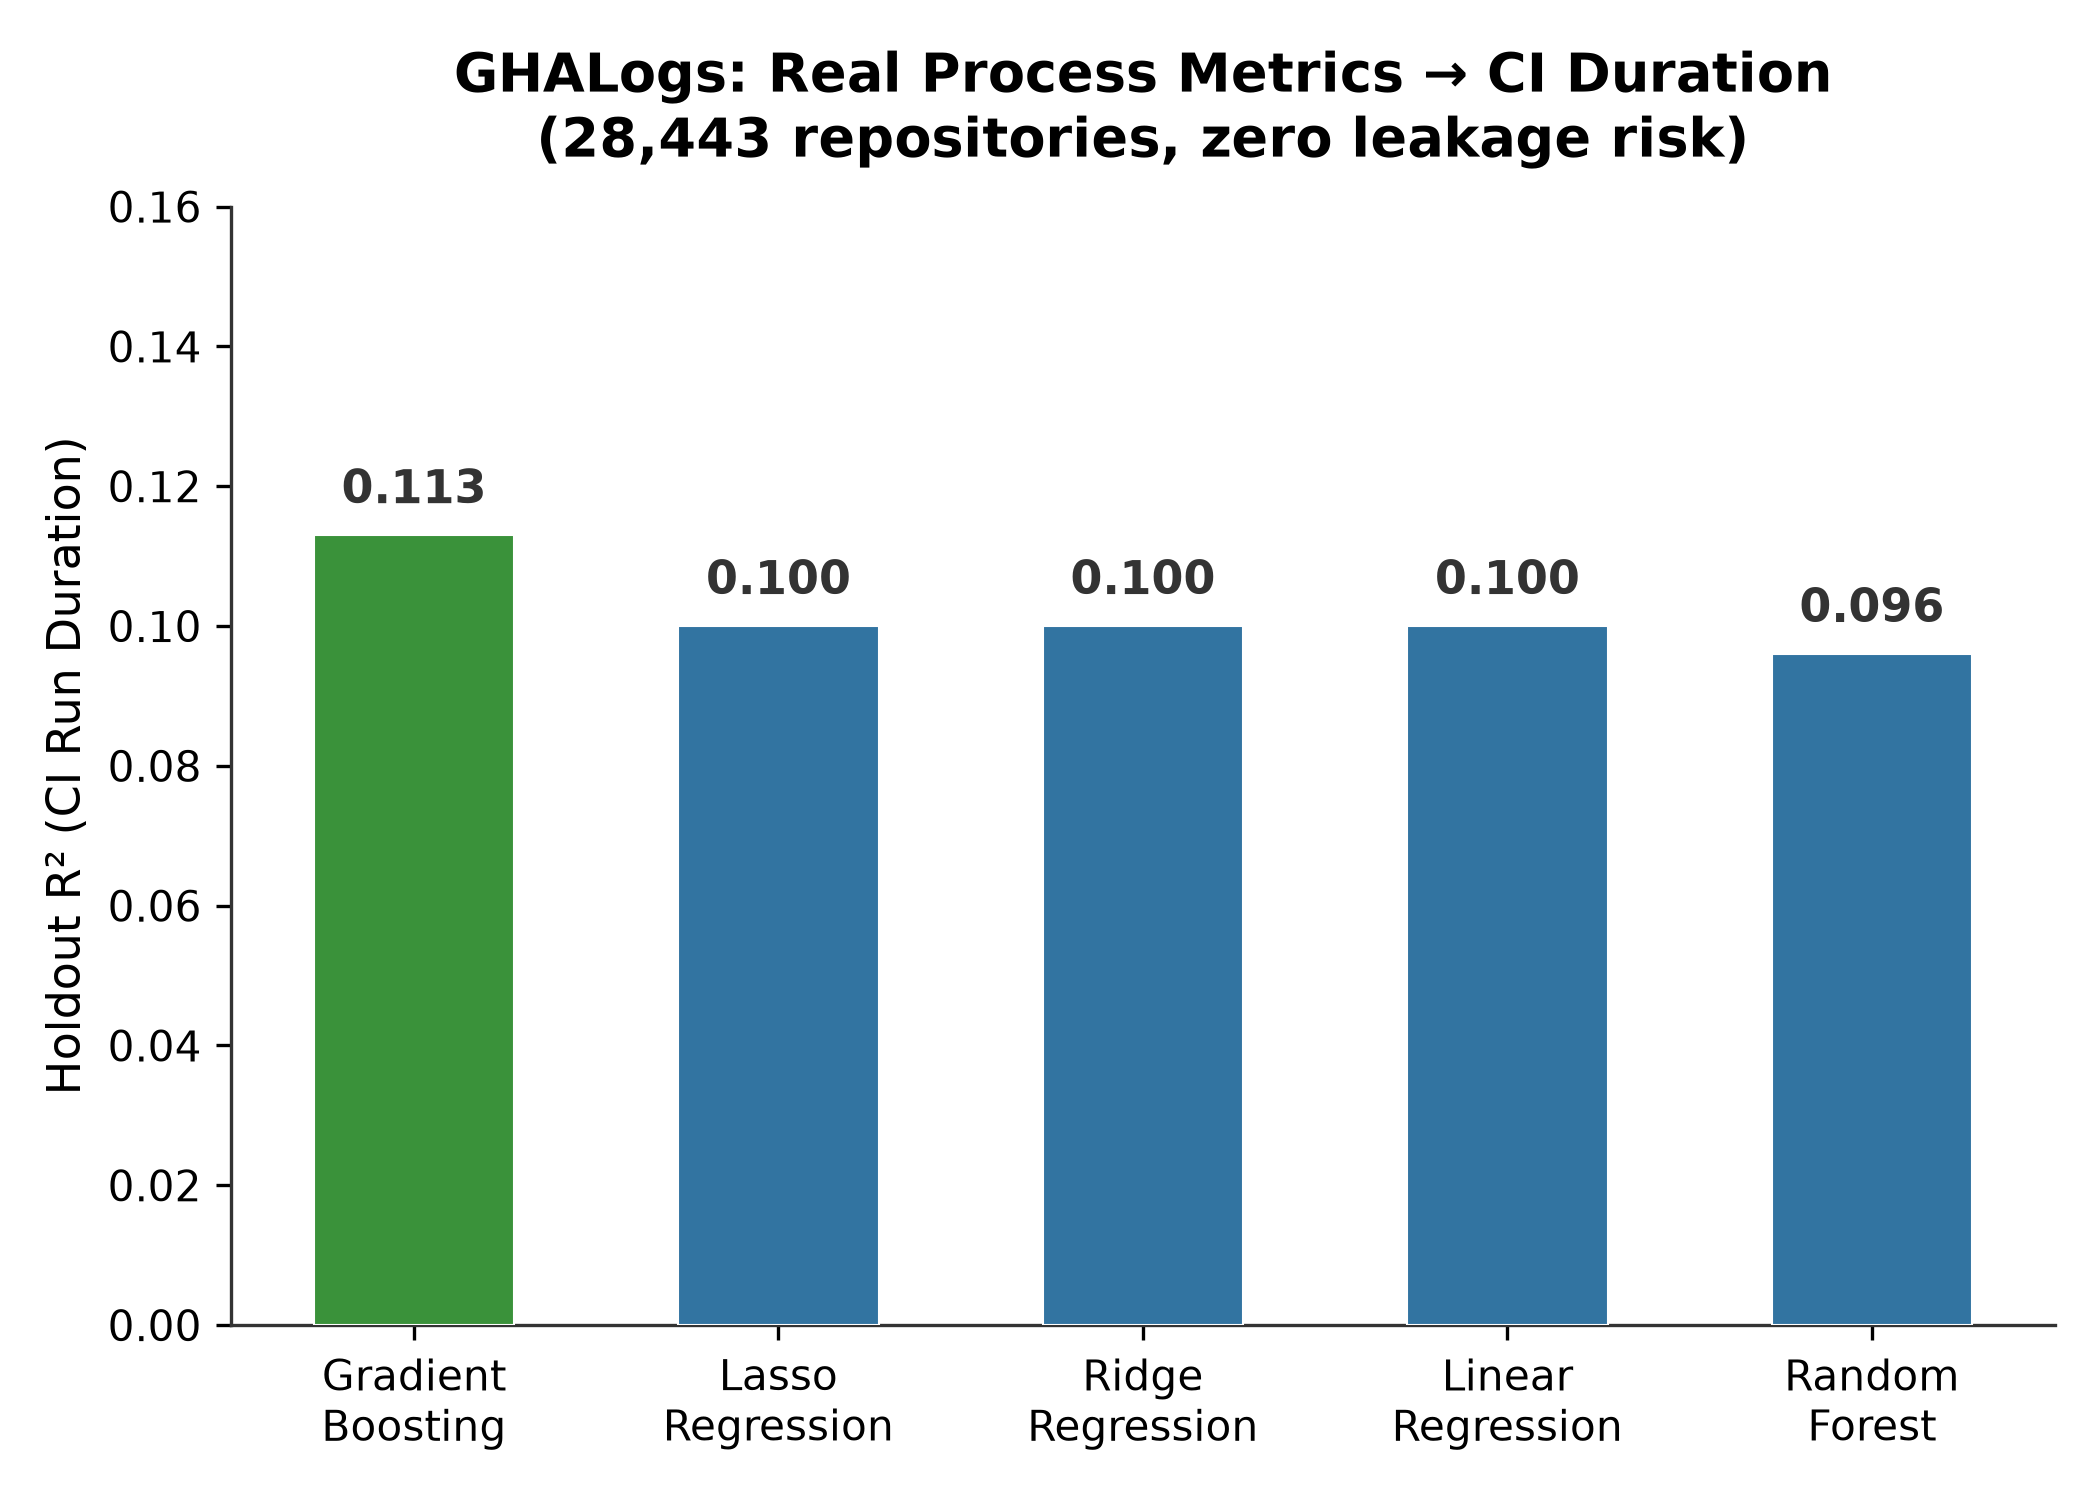
\includegraphics[width=0.85\textwidth]{images/fig_14_ghalogs_validation.png}
\caption{GHALogs cross-sectional validation: holdout R² per model
predicting CI run duration from real repository process characteristics
across 28,443 repositories.\label{fig:ghalogs_validation}}
\end{figure}

Figure~\ref{fig:ghalogs_validation} plots the per-model holdout \(R^2\) shown in Table~\ref{tab:ghalogs}.
28,443 repositories, chronological (push-date-sorted) 80/20 split,
target is mean total CI run duration in seconds across each repository's
up to five sampled runs (mean 1,327s, median 311s, heavily
right-skewed). The top feature by Random Forest importance is
\texttt{mean\_n\_steps} (48.6\%) -- largely definitional (more workflow
steps take longer), analogous to the near-tautological ``System
Availability'' feature already flagged in the synthetic
feature-importance analysis (Section~\ref{sec:feature_importance}). The remaining
\textasciitilde51\% of importance is genuine process/popularity signal:
success rate, codebase size, repository age, PR/issue counts, and
popularity metrics. \textbf{All five models' 95\% bootstrap confidence
intervals (2,000-resample pairs/case bootstrap on the holdout
predictions, identical procedure to the synthetic-domain analysis in
Section~\ref{sec:bootstrap_ablation}) exclude zero} -- this is the only
real-world validation in this paper where every model's interval
clears significance, and it is the largest sample by a wide margin
(\(n=28{,}443\)). The modest but real, statistically significant, leakage-free
signal (\(R^2 \approx 0.10\)--\(0.11\)) at real-world scale directly
supports RQ1's ``genuine, if modest, predictive signal'' framing -- this
time with no leakage-related caveats needed at all, and now with the
uncertainty quantification the synthetic domains already receive -- and, alongside
TravisTorrent, provides a second modern, cross-sectional real-world CI
dataset.

\subsubsection{SQuaD (Real Process Metrics, Cross-Sectional
Defect-Proneness)}\label{sec:squad}

SQuaD~\cite{squad2025} provides 62,449 release-level process metrics (lines of
code, code churn, commit-author count, change-set size, release age)
across 440 open-source projects in the \texttt{process\_metrics.csv} slice we
downloaded and use here (the full published SQuaD dataset covers 450
mature open-source projects across nine static-analysis tools; the
440-project figure is specific to the process-metrics component this
validation uses, not a discrepancy with the dataset's own description).
Unlike TravisTorrent, Perfherder, and
GHALogs, none of SQuaD's metrics map by name to PRESTO's own 164-metric
registry, so this validation cannot check the copula's 84 hand-specified
correlation coefficients directly against real values (that would
require metrics like Test Pass Rate or Build Success Rate, which SQuaD
does not record). What it can test, and does, is the paper's broader RQ1
thesis -- do real process characteristics predict a real outcome -- on a
fourth, independent dataset and a different outcome variable: defect-fix
rate.

\textbf{Adaptation.} We aggregated to one row per project (408 of 440
projects with \(\geq 5\) observed releases) rather than using all 62,449
release-level rows, since a single project
(\texttt{apache\#servicemix-bundles}) accounts for 27\% of raw rows and
would dominate a release-level split. Features are per-project means of
the available process metrics (LOC, churn, change-set size,
commit-author count, release age) plus their variance where available;
the target is mean per-release defect-fix count (\texttt{n\_fix}), a
standard process-metrics-predict-defects proxy in the SE literature
\cite{nagappan2006}. As with GHALogs, no historical target values are
used as features, so this is a clean, leakage-free cross-sectional test. Table~\ref{tab:squad} reports the results.

{\def\LTcaptype{none} % do not increment counter
\begin{table}[H]
\centering
\caption{SQuaD cross-sectional defect-fix-rate prediction results.\label{tab:squad}}
\begin{tabularx}{\linewidth}{LLLLL}
\toprule
\textbf{Model} & \textbf{Holdout \(R^2\)} & \textbf{95\% Bootstrap CI} & \textbf{Holdout MAE} &
\textbf{Holdout RMSE} \\
\midrule
\textbf{Random Forest} & \textbf{0.402} & [\(-0.245\), 0.748] & 81.65 & 148.77 \\
Gradient Boosting & \(-0.325\) & [\(-1.408\), 0.398] & 106.84 & 221.52 \\
Lasso Regression & \(-0.409\) & [\(-2.554\), 0.665] & 107.55 & 228.38 \\
Ridge Regression & \(-0.442\) & [\(-2.651\), 0.670] & 108.49 & 231.08 \\
Linear Regression & \(-0.455\) & [\(-2.685\), 0.670] & 109.11 & 232.06 \\
\bottomrule
\end{tabularx}
\end{table}
}

Random Forest achieves \(R^2 = 0.402\) -- nominally the strongest point
estimate of this paper's four \emph{dataset-level, process-metric-only
(non-AR)} real-world results (i.e., excluding
TravisTorrent's best single project, youtube-dl at \(R^2 = 0.475\),
which is not representative of that dataset's median project of
\(0.005\), and excluding Mozilla Perfherder's higher with-AR figures of
0.574--0.913, which reflect autoregressive persistence rather than SDLC
process signal and are not the same kind of result -- see
Section~\ref{sec:perfherder}) -- but the 95\% bootstrap CI (2,000-resample
pairs/case bootstrap, same procedure as Section~\ref{sec:bootstrap_ablation}) is
\([-0.245, 0.748]\), which \textbf{includes zero}. On a holdout of
roughly 82 projects (20\% of 408), this point estimate cannot be
distinguished from ``no better than the mean'' at conventional
confidence levels. We report it as the strongest point estimate among
this paper's dataset-level real-world results because that is what it
is, but ``strongest point estimate'' and ``statistically significant''
are different claims, and only the second would license the word
``confirm.''
It exceeds even the synthetic domains' best without-AR
figure (0.362, Card Payment). Every linear model fails, consistent with every other dataset examined in this paper:
process-metric feature spaces are non-linear enough that tree-based
ensembles are needed, not a synthetic-data artifact. The top features by
Random Forest importance are release age (30.8\%), churn (20.3\%), and
commit-author count (17.6\%) -- all correlate positively with defect-fix
rate (\(\rho = 0.44\), \(0.34\), \(0.38\) respectively), directionally
consistent with classical process-metrics literature (older,
higher-churn, higher-author-count releases accumulate more fixes) though
not a direct test of any specific PRESTO copula coefficient, per the
scope note above.

\paragraph{From Defects to Vulnerabilities: A Harder Security
Target}\label{sec:squad_vuln}

SQuaD ships one more linked field we had not yet used:
\texttt{cve\_data.csv}, 5,294 CVE-linkage rows spanning 175 of SQuaD's
440 projects and 1,479 distinct CVE IDs, sourced from GitHub
Dependabot/security-advisory data. Defect-fix rate and vulnerability
count are related but distinct outcomes -- a bug-fix commit reflects
internal code-quality process, while a CVE disclosure reflects both
process \emph{and} external exposure (how widely used a project is, how
actively security researchers and dependency scanners target it). We
reused the same 408-project aggregation unit and the same process-metric
feature set as the defect-fix-rate validation above, changing only the
target: \texttt{log1p(cve\_count)}, the number of distinct CVEs linked
to a project (247 of 408 qualifying projects have zero; the raw count is
heavily right-skewed, topping out at 222 for
\texttt{apache\#ofbiz-framework}, hence the log transform). Table~\ref{tab:squad_vuln} reports the results.

{\def\LTcaptype{none} % do not increment counter
\begin{table}[H]
\centering
\caption{SQuaD cross-sectional CVE-count prediction results.\label{tab:squad_vuln}}
\begin{tabularx}{\linewidth}{LLLLLL}
\toprule
\textbf{Model} & \textbf{CV \(R^2\)} & \textbf{Holdout \(R^2\)} & \textbf{95\% Bootstrap CI} & \textbf{Holdout MAE} & \textbf{Holdout RMSE} \\
\midrule
\textbf{Random Forest} & \(0.059 \pm 0.270\) & \textbf{0.245} & [0.053, 0.370] & 0.958 & 1.332 \\
Gradient Boosting & \(-0.194 \pm 0.545\) & 0.201 & [\(-0.053\), 0.407] & 0.991 & 1.371 \\
Lasso Regression & \(-0.037 \pm 0.042\) & \(-0.032\) & [\(-0.128\), \(-0.000\)] & 1.184 & 1.558 \\
Ridge Regression & \(-0.964 \pm 1.215\) & \(-0.837\) & [\(-2.329\), 0.066] & 1.291 & 2.078 \\
Linear Regression & \(-1.854 \pm 2.277\) & \(-0.949\) & [\(-2.468\), 0.042] & 1.317 & 2.140 \\
\bottomrule
\end{tabularx}
\end{table}
}

Random Forest again wins (\(R^2 = 0.245\)), and its 95\% bootstrap CI
\([0.053, 0.370]\) excludes zero -- unlike the defect-fix-rate result
immediately above, this one is statistically significant, despite being
the numerically smaller point estimate. Every linear model
fails, the same non-linearity pattern observed on every other real
dataset in this paper. The result is real, significant, and appreciably weaker in point-estimate terms than
the same features' \(R^2 = 0.402\) (not significant) on defect-fix rate, which is the
expected direction: CVE disclosure count is confounded by exposure
surface in a way defect-fix rate is not, so process metrics alone should
carry, and here do carry, less of the outcome's variance. We read this
as a substantive finding about the limits of process-metrics-only
vulnerability prediction, not a weaker version of the same result --
predicting \emph{how many bugs get fixed} from process signals is a
meaningfully easier problem than predicting \emph{how many disclosed
vulnerabilities accumulate}, and a paper that only reported the easier,
better-looking (but not significant) number would be giving an incomplete
and, on this evidence, misleading picture of what SDLC
process metrics can and cannot do.

\paragraph{Enrichment with Real Static-Analysis Code-Quality Features}\label{sec:squad_enriched}

Both SQuaD analyses above use only \texttt{process\_\allowbreak metrics.csv} (LOC, churn,
commit-author count, release age) -- SQuaD's full published release
includes raw per-file/per-issue output from three static-analysis tools
(SonarQube, PMD, CK) that we had not previously downloaded, at a
combined uncompressed size (1.2\,TB across these three files alone)
that made a full in-memory load infeasible. We aggregated each to
project-release granularity with a streaming SQL engine (DuckDB,
single-pass scan, no full-file materialization in memory) -- SonarQube's
per-project-release \texttt{measures\_*} columns (bugs, code smells,
cognitive complexity, coverage, duplication,
maintainability/reliability/security ratings, technical-debt ratio),
PMD's violation counts by priority, and CK's per-class object-oriented
complexity metrics (WMC, CBO, DIT, LCOM, RFC) averaged to per-release --
then rolled up to per-project means (matching the \(\geq 5\)-release
aggregation unit used throughout this section) and joined onto the
existing feature set. Coverage is incomplete: of the 408 qualifying
projects, 352 have SonarQube data, 345 have PMD data, and 311 have CK
data; missing values are median-imputed, consistent with this paper's
handling of missing values elsewhere.

This is a genuine Code-quality-phase signal that the paper's SQuaD
validation previously lacked entirely -- unlike
\texttt{process\_\allowbreak metrics.csv}'s churn/LOC/author-count features, which are
Project/Process-phase metrics, SonarQube's ratings and PMD/CK's
violation and complexity counts are exactly the kind of static-analysis
output PRESTO's own metric registry treats as a distinct SDLC phase.
With this enrichment (48 features, up from 13), Random Forest's holdout
\(R^2\) rises from 0.402 to \textbf{0.483}, and the 95\% bootstrap CI
narrows from \([-0.245, 0.748]\) to \([-0.037, 0.738]\) -- moving
substantially closer to significance but, at a hair's width, still
\textbf{not} crossing zero. Feature importances confirm the new sources
are contributing real signal, not noise: \texttt{sq\_\allowbreak mean\_\allowbreak measures\_\allowbreak classes}
(project size proxy, 4.6\%), \texttt{sq\_\allowbreak mean\_\allowbreak measures\_\allowbreak bugs} (2.3\%),
PMD violation counts (2.2\%, 2.0\%), SonarQube cognitive complexity
(2.1\%), and CK's mean class coupling and size (1.3\%, 1.2\%) all rank
inside the top 16 features, ahead of several of the original
process-metrics features -- but the four original process/churn
features (release age, commit-author count, churn, churn variability)
still dominate the top four ranks combined (\(\approx\)60\% of total
importance).

We report this as an honest near-miss, not a resolved result: the CI
still includes zero, the coverage gaps required imputation for roughly
13--24\% of projects depending on source, and this is a single 80/20
split rather than a repeated-resampling estimate, so the improvement
should not be over-read. But the direction is informative -- adding
genuine Code-quality-phase static-analysis features narrows, rather
than widens, the gap to significance, which is the outcome this paper's
broader thesis (SDLC process signals carry real predictive value) would
predict if SQuaD's original null result were partly an artifact of an
incomplete feature set rather than a ceiling on what process signals
can predict. Full results, per-model bootstrap CIs, and the complete
feature-importance table:
\texttt{research-\allowbreak data/\allowbreak presto/\allowbreak real-\allowbreak data/\allowbreak squad/\allowbreak SQUAD\_\allowbreak ENRICHED\_\allowbreak STATIC\_\allowbreak ANALYSIS\_\allowbreak RESULTS.md}.

\begin{sloppypar}
We also examined SQuaD's refactoring-detection outputs
(\texttt{pp\_rminer.csv}, RefactoringMiner-style Java/C++ events, 48
rows confined to a single project; \texttt{pyref.csv}, PyRef
Python-refactoring events, 752 rows across 75 projects, averaging
roughly 10 events per project) as a candidate fifth real-data analysis.
Both are too sparse for a reliable per-project aggregation at the
standard \(\geq 5\)-observation threshold used throughout this section,
so we do not report a refactoring-rate validation here; a dataset with
denser refactoring coverage would be needed to test that specific
hypothesis honestly.
\end{sloppypar}

\subsection{Deployment Considerations}\label{sec:deployment}

PRESTO's trained models are lightweight (under 50 MB) and produce
predictions in under 100 ms per release, making them suitable for
integration into CI/CD pipelines as a pre-merge gate or canary promotion
criterion. Operationalizing such ML models in production remains a
recognized challenge in MLOps
practice~\cite{shankar2022, diazdearcaya2024}. Production deployment
would require integration with existing metric collection infrastructure
(CI/CD, APM, test management systems), periodic model retraining as
organizational processes evolve, calibration against actual production
outcomes to establish site-specific prediction accuracy, and monitoring
for concept drift as the relationship between SDLC practices and
outcomes shifts over time. From an SRE perspective, automated SDLC-based
prediction reduces toil by replacing manual release-readiness checklists
with data-driven risk scores.

We emphasize that reported \(R^2\) values were obtained on synthetic
data and represent an upper bound; site-specific validation is required
before operational reliance.

\subsection{Potential Applications}\label{sec:applications}

Based on the demonstrated predictive signal from SDLC metrics
(Section~\ref{sec:cross_domain}), we identify
potential applications warranting real-world investigation:

\begin{itemize}
\item
  \textbf{Release risk scoring:} Flagging releases where SDLC metric
  patterns deviate from historical norms associated with high uptime,
  enabling targeted pre-deployment review
\item
  \textbf{Test environment investment prioritization:} Organizations can
  use the feature importance rankings
  (Section~\ref{sec:feature_importance}) to prioritize
  infrastructure investments
\item
  \textbf{Early warning for deployment decisions:} Even modest
  predictive accuracy can be operationally valuable when combined with
  other decision inputs, particularly for high-stakes releases
\item
  \textbf{Process metric benchmarking:} The cross-domain results provide
  a framework for comparing SDLC metric profiles across teams or
  organizations
\end{itemize}

We deliberately avoid quantifying dollar-value business impact, as such
estimates would require real-world deployment data that this study does
not provide. The contribution here is demonstrating feasibility and
identifying which SDLC metrics carry predictive signal, not prescribing
operational thresholds.

\section{Threats to Validity}\label{sec:threats}

Following established guidelines for empirical software engineering
research, we discuss threats to validity organized by category.

\subsection{Internal Validity}\label{sec:internal_validity}

Internal validity concerns whether the observed relationship between
SDLC metrics and performance outcomes reflects genuine predictive signal
or artifacts.

\textbf{Autoregressive-Feature Dependence:} With 273 engineered features
including 32 derived from the target variable, AR-feature dependence
(previously mislabeled outright ``target leakage'' before the R2
rolling-window fix) is a primary concern, though only 20 of the 32 were
ever a genuine same-row leakage bug -- an instance of the temporal
leakage vectors catalogued in our build-prediction taxonomy
\cite{mishra2026leakage}. We address this directly by reporting all
results both with and without AR features (Section~\ref{sec:results}). The without-AR
results (\(R^2 = 0.26\)--\(0.36\)) represent our conservative estimate
of genuine SDLC predictive signal.

\textbf{Feature Engineering Bias:} Feature engineering was informed by
domain knowledge, introducing risk that features were designed to fit
patterns in the synthetic data. \emph{Mitigation:} Feature engineering
logic is identical across all three domains and was defined before
observing results.

\textbf{Hyperparameter Selection:} Default or conservative
hyperparameters were used (e.g., Random Forest with 100 trees, max depth
10). No hyperparameter optimization was performed, reducing overfitting
risk but potentially underestimating achievable accuracy.

\textbf{Copula Correlation Specification:} The 84 inter-metric
correlations in the Gaussian copula were specified by the authors based
on domain expertise. If these correlations encode assumptions that align
with the prediction models, results may be optimistic.
\emph{Mitigation:} Correlation specifications are published in full as
YAML configuration files for independent review.

\textbf{Cross-Domain Correlation Non-Independence:} The same limitation
applies across, not just within, domains. \texttt{generate.py} loads a
single \texttt{correlation\_templates.yaml} once per run and passes the
identical 84-pair correlation configuration to all three domains'
generation calls unchanged -- only each domain's marginal distributions,
temporal dynamics, and release cadence (\texttt{domain\_profiles.yaml})
vary. This means the Cross-Domain Validation result
(Section~\ref{sec:cross_domain}, all three domains achieving positive
without-AR \(R^2\) in a narrow 0.255--0.362 band) is not three
independent confirmations of the same finding; it is one correlation
specification's signal recovered under three different marginal/temporal
configurations. The consistency across domains is still informative --
it shows the recovered signal is not an artifact of one domain's
specific marginal distributions -- but it should not be read as though
three separately-specified, independently-validated domains all
happened to agree.

\textbf{Near-Tautological Features Ablation:} System Availability
(\%), a performance testing metric, is semantically related to the
target variable System Uptime (\%) and ranks \#2 in Random Forest's
Gini-based feature importance on the primary domain without AR features
(14.8\%, consistent with the 14.9\% figure this caveat originally
reported; the RQ2 table in Section~\ref{sec:feature_importance} uses permutation importance
instead, where this feature does not rank in the top 15). Rather than
only flagging the overlap, we tested it directly: we removed System
Availability (\%) and every feature engineered from it, retrained Random
Forest with unchanged hyperparameters, and compared holdout \(R^2\)
across all three domains (without AR features; full results including
the with-AR condition:
\texttt{research-data/\allowbreak presto/\allowbreak code/\allowbreak synthetic\_\allowbreak data\_\allowbreak generator/\allowbreak M9\_\allowbreak SYSTEM\_\allowbreak AVAILABILITY\_\allowbreak ABLATION\_\allowbreak EVIDENCE.md}). Table~\ref{tab:m9_ablation} reports the results.

{\def\LTcaptype{none} % do not increment counter
\begin{table}[H]
\centering
\caption{System Availability (\%) ablation results, per domain.\label{tab:m9_ablation}}
\begin{tabular}{@{}
  >{\raggedright\arraybackslash}p{(\linewidth - 8\tabcolsep) * \real{0.1667}}
  >{\raggedleft\arraybackslash}p{(\linewidth - 8\tabcolsep) * \real{0.2222}}
  >{\raggedleft\arraybackslash}p{(\linewidth - 8\tabcolsep) * \real{0.2222}}
  >{\raggedleft\arraybackslash}p{(\linewidth - 8\tabcolsep) * \real{0.2222}}
  >{\raggedright\arraybackslash}p{(\linewidth - 8\tabcolsep) * \real{0.1667}}@{}}
\toprule
\begin{minipage}[b]{\linewidth}\raggedright
\textbf{Domain}
\end{minipage} & \begin{minipage}[b]{\linewidth}\raggedleft
\textbf{RF Holdout R² (full)}
\end{minipage} & \begin{minipage}[b]{\linewidth}\raggedleft
\textbf{RF Holdout R² (ablated)}
\end{minipage} & \begin{minipage}[b]{\linewidth}\raggedleft
\textbf{\(\Delta\)}
\end{minipage} & \begin{minipage}[b]{\linewidth}\raggedright
\textbf{New top feature after ablation}
\end{minipage} \\
\midrule
ABC Cloud (primary) & 0.268 & \(-0.042\) & \(-0.310\) & Test Environment
Availability (\%), 23.0\% \\
Card Payment & 0.339 & 0.706 & \(+0.367\) & UAT Environment Stability
(\%), 30.9\% \\
XYZ Sales & 0.255 & 0.168 & \(-0.087\) & UAT Environment Stability (\%),
42.1\% \\
\bottomrule
\end{tabular}
\end{table}
}

The result is not what the ``tautological noise'' framing predicts, and
it is not consistent across domains. On the primary domain, removing the
feature \emph{collapses} the model below zero -- System Availability
(\%) is load-bearing, not redundant, so the original caveat understated
rather than overstated its importance there. On Card Payment, removing
it substantially \emph{improves} \(R^2\), indicating the feature was
actively harmful (adding noise or multicollinearity) rather than
tautological in that domain. On XYZ Sales, removal produces a modest
decline, closer to what ``near-tautological but not essential'' would
predict. This cross-domain inconsistency plausibly connects to the same
mechanism documented in the ``Bootstrap Confidence Intervals and
Target-Correlation Ablation'' analysis (Section~\ref{sec:bootstrap_ablation}): the copula's
global positive-semi-definite correction (Higham's alternating
projections) couples variables the config file's section structure
implies are independent, so a single feature's causal role is not
necessarily stable across differently-configured domains. Practitioners
should not assume this feature's importance is an artifact to be
discounted uniformly -- its actual contribution is domain-specific and,
in the primary domain at least, real rather than tautological.

\subsection{External Validity}\label{sec:external_validity}

External validity concerns generalizability of findings to real-world
systems.

\textbf{Synthetic Data (Critical):} The most critical limitation is
exclusive reliance on synthetic data. This choice is necessitated by the
complete absence of public datasets combining SDLC process metrics with
runtime performance outcomes; no such benchmark exists in UCI, Kaggle,
Zenodo, PROMISE, or any repository we surveyed. Organizations treat the
required telemetry as proprietary. While our copula-based generator
produces statistically grounded datasets calibrated to DORA benchmarks,
synthetic data cannot capture:

\begin{itemize}
\item
  Organizational culture, team dynamics, and process maturity
\item
  Domain-specific performance failure modes
\item
  Real-world data quality issues (missing metrics, instrumentation gaps)
\item
  Emergent behaviors from human factors and market pressures
\end{itemize}

\emph{Partial Mitigation:} Our TravisTorrent validation
(Section~\ref{sec:travistorrent}) demonstrates that
SDLC metrics contain predictive signal for build duration in real
open-source projects (\(R^2\) up to 0.475), partially addressing this
limitation. However, the target variable differs (build duration
vs.~system uptime), only 4 of 8 SDLC phases are available, and the
median \(R^2\) across projects (0.005) is only marginally positive,
indicating that infrastructure confounders still dominate in most
projects. Full validation on production SDLC data with runtime
performance outcomes remains essential.

\textbf{Domain Coverage:} We evaluated three synthetic application
domains (cloud platform, CRM/SaaS, payment processing) and seven
open-source projects from the TravisTorrent dataset. Findings may not
transfer to embedded systems, mobile applications, real-time systems, or
safety-critical software where performance characteristics differ
fundamentally.

\subsection{Construct Validity}\label{sec:construct_validity}

Construct validity concerns whether measurements capture the intended
constructs.

\textbf{Target Variable:} System Uptime (\%) captures availability but
not all dimensions of system performance (latency, throughput, error
rates, resource efficiency). A multi-target formulation would provide
more complete performance prediction.

\textbf{SDLC Metric Coverage:} Our 164 metrics span 8 SDLC phases but
may omit relevant factors such as architectural complexity, dependency
health, team composition, and technical debt accumulation rates.

\textbf{Temporal Granularity:} Release-level aggregation may mask
important within-release dynamics. Systems with continuous deployment
may require finer-grained temporal resolution.

\subsection{Conclusion Validity}\label{sec:conclusion_validity}

Conclusion validity concerns statistical reliability of findings.

\textbf{Sample Size:} The feature-to-sample ratios before feature
selection (1.77, 1.51, and 2.01 features per training sample for ABC
Cloud, XYZ Sales, and Card Payment respectively, i.e.\ 241:136, 241:160,
241:120, using each domain's 80\% training partition rather than its
full release count) fall roughly 15--20 times short of the classical guideline of at
least 10 samples per feature, not the reverse -- this is a genuine
limitation, not a mitigated one. Overfitting risk remains
despite tree-based model robustness
(Section~\ref{sec:model_char}). After PA-RFE feature reduction
(Section~\ref{sec:parfe_results}), the ratios improve substantially --
to roughly 0.6:1 through 0.2:1 (26--81 selected features against a
136-row training partition) -- though this reduction did not reliably
improve test-set \(R^2\), so it should be read as a partial mitigation
of the ratio itself, not of the underlying overfitting risk. The consistent
cross-domain results (\(R^2 = 0.26\)--\(0.36\)) provide further partial
mitigation, though see the comparison-family caveat below before
reading that consistency as strong evidence on its own.

\textbf{Comparison-Family Size and Multiple Comparisons:} This paper
reports a large number of independent ``best of 5 models'' selections --
at minimum: 3 synthetic domains x 2 AR conditions, 7 TravisTorrent
projects, 3 Perfherder signatures x 2 conditions, 2 Perfherder
bug-enriched signatures x 2 conditions, GHALogs, SQuaD defect-fix, SQuaD
CVE-count, plus 24 nested-CV tuning results (Section~\ref{sec:m3_tuning})
and 9 feature-selection-method comparisons (Section~\ref{sec:parfe_results})
-- on the order of 150 reported comparisons in total, from which the
paper's headline maxima (e.g.\ TravisTorrent's best-of-seven
\(R^2=0.475\), SQuaD's \(R^2=0.402\)) are drawn. We do not apply a formal
multiple-comparisons correction (e.g.\ Bonferroni or Benjamini-Hochberg)
across this family: the comparisons are largely exploratory and
diagnostic rather than confirmatory hypothesis tests of a single
pre-registered claim, and a strict correction would be an odd fit for a
paper whose contribution is partly the diagnostic comparisons themselves
(e.g.\ showing that an untuned linear model collapses while a tuned one
does not). We flag this explicitly, however, because we hold a competing
method to a stricter standard elsewhere in this paper: the reimplemented
Siegmund-style baseline (Section~\ref{sec:model_char}) is criticized for
testing up to 105 candidate interaction pairs without
multiple-comparisons correction against only 136 training samples, and a
careful reader is right to ask why this paper's own reporting practice
is not held to the same standard. The honest answer is that it is not,
and any single reported maximum in this paper -- particularly
TravisTorrent's best-of-seven and the per-domain ``best model'' figures
-- should be read as one draw from a family of comparisons this size,
not as a value selected against a pre-registered null.

\textbf{Honest Reporting:} Unlike prior synthetic-data studies reporting
\(R^2 > 0.95\), we separate temporal autocorrelation from genuine SDLC
prediction through the dual-condition evaluation in
Section~\ref{sec:results}. This transparency enables
accurate expectations for real-world deployment.

\subsection{Summary of Validity Assessment}\label{sec:validity_summary}

Table~\ref{tab:validity} consolidates the severity and mitigation
status of each threat category.

{\def\LTcaptype{none} % do not increment counter
\begin{table}[H]
\centering
\caption{Summary of validity threats and mitigation status.\label{tab:validity}}
\begin{tabular}{@{}
  >{\raggedright\arraybackslash}p{(\linewidth - 6\tabcolsep) * \real{0.2500}}
  >{\raggedright\arraybackslash}p{(\linewidth - 6\tabcolsep) * \real{0.2500}}
  >{\raggedright\arraybackslash}p{(\linewidth - 6\tabcolsep) * \real{0.2500}}
  >{\raggedright\arraybackslash}p{(\linewidth - 6\tabcolsep) * \real{0.2500}}@{}}
\toprule
\begin{minipage}[b]{\linewidth}\raggedright
\textbf{Threat Category}
\end{minipage} & \begin{minipage}[b]{\linewidth}\raggedright
\textbf{Severity}
\end{minipage} & \begin{minipage}[b]{\linewidth}\raggedright
\textbf{Key Concern}
\end{minipage} & \begin{minipage}[b]{\linewidth}\raggedright
\textbf{Mitigation Status}
\end{minipage} \\
\midrule
Internal & Medium & Feature engineering bias & Partially mitigated \\
External & \textbf{Critical} & Synthetic data only &
\textbf{Unmitigated} \\
Construct & Medium & Metric validity & Acknowledged \\
Conclusion & High & Overfitting risk & Partially mitigated \\
\bottomrule
\end{tabular}
\end{table}
}

\textbf{Critical Message:} The external validity threat from
synthetic-only validation is the primary limitation. While our results
suggest SDLC metrics may predict performance, this finding requires
real-world validation before any operational deployment recommendations
can be made with confidence.

\section{Discussion and Future Work}\label{sec:discussion}

\subsection{Summary of Findings}\label{sec:summary_findings}

A striking pattern in this synthetic design: test environment stability
shows roughly 11x the importance of code quality. Test environment
availability alone (42.9\% importance) exceeds all code-phase metrics
combined (4.8\%). We flag this as a hypothesis worth testing on real
data, not a confirmed finding -- the copula generator's inter-metric
correlations, including this one, are hand-specified rather than
independently emergent, so this pattern may partly reflect the
generator's configuration rather than an independent discovery (Section~\ref{sec:internal_validity}). GHALogs' real-data validation (Section~\ref{sec:ghalogs}) shows a broadly
compatible pattern (process/quality characteristics carry real signal
beyond simple size proxies), but does not by itself confirm the specific
11:1 ratio.

Across the four research questions, SDLC process metrics provide genuine
but modest predictive signal (\(R^2 = 0.26\)--\(0.36\), RQ1), with
testing infrastructure metrics dominating feature importance (53.6\%,
RQ2). Tree-based ensembles outperform \emph{untuned} linear models due
to multicollinearity in the high-dimensional feature space (RQ3), but
nested-CV alpha tuning (Section~\ref{sec:m3_tuning}) shows this is a
hyperparameter-choice artifact rather than a general finding: properly
tuned linear models exceed Random Forest in 2 of 3 domains, and only the
primary domain (ABC Cloud Provider) still favors trees after tuning.
Autoregressive persistence is the single most influential factor (RQ4).
PA-RFE, reimplemented from the paper's own pseudocode (Section~\ref{sec:parfe_results}),
reliably guarantees cross-phase feature coverage but its test-set
predictive accuracy does not reliably beat simpler baselines.

\subsection{Practical Implications}\label{sec:practical_implications}

Subject to real-world validation, our findings tentatively suggest
actionable guidance for practitioners, though we hedge this
recommendation pending confirmation on real data (Section~\ref{sec:internal_validity}):
investing in test infrastructure stability before optimizing code
quality metrics may be worthwhile. Test environment availability
dominates feature importance at 42.9\% in this synthetic design (Section~\ref{sec:feature_importance}), which would mean that teams chasing code coverage targets while
tolerating flaky test environments are optimizing the wrong variable --
but this should be validated against real SDLC data before being treated
as an operational recommendation. For SDLC-based prediction tasks, tree-based
ensembles are a reasonable default choice, but not an unconditional one:
nested-CV alpha tuning (Section~\ref{sec:m3_tuning}) shows a properly regularized
linear model can match or exceed them, so practitioners with the budget for a
brief hyperparameter search should not rule out Ridge or Lasso based on an
untuned comparison alone.

Historical uptime is a legitimate and powerful predictor, and teams
should track performance trends across releases to feed this signal into
their models. Even modest predictive accuracy (\(R^2 \approx 0.3\))
provides operational value for release risk assessment when combined
with other decision inputs, particularly for flagging releases whose
SDLC metric profiles diverge from patterns historically associated with
stable deployments. Additionally, the synthetic data generator enables
organizations to prototype prediction systems and validate their metric
instrumentation before committing to full production telemetry
pipelines.

\subsection{Limitations}\label{sec:limitations}

The primary limitations are synthetic-only core validation, limited
domain coverage (three application types), author-specified copula
correlations, a single target variable (uptime), and high
feature-to-sample ratios. We also note that our current target variable
(system uptime) captures only one dimension of production performance.
Real-world teams track SLO breaches across multiple golden signals
(latency, traffic, errors, saturation), and a production-grade
prediction system would need to model p99 latency and error budgets
alongside uptime. Section~\ref{sec:threats} provides
detailed threat analysis and mitigation status for each concern.

\subsection{Future Work}\label{sec:future_work}

The most critical next step is real-world validation through
organizational partnerships that provide production performance metrics
alongside full 8-phase SDLC data. Such partnerships would also enable
validation against operational SLO definitions rather than synthetic
uptime targets. Beyond that broad goal, this paper's own results point
to several specific, concrete next steps -- listed roughly in order of
tractability, from ``a follow-up script on data we already have'' to
``requires new data collection'' -- for researchers who want to build
directly on this work rather than start from a blank page:

\begin{enumerate}
\item \textbf{Close the SQuaD near-miss.} The static-analysis-enriched
  defect-fix-rate result (Section~\ref{sec:squad}) moved from
  \(R^2=0.402\) (95\% CI \([-0.245, 0.748]\)) to \(R^2=0.483\) (95\% CI
  \([-0.037, 0.738]\)) -- tantalizingly close to significance but not
  there. Three concrete, low-cost paths forward on data this paper
  already has partial access to: (a) improve SonarQube/PMD/CK coverage
  beyond the 352/345/311-of-408 projects achieved here (the remaining
  gap is median-imputed, which dilutes signal); (b) incorporate the
  four raw static-analysis files this paper deliberately deprioritized
  for tractability (JaSoMe, Understand, CodeScene, RefactoringMiner --
  up to 389\,GB each), which likely carry additional Code-quality-phase
  signal; (c) replace the single 80/20 split used here with
  repeated-resampling or nested cross-validation to get a tighter,
  less split-dependent confidence interval, the same fix that mattered
  for the linear-model tuning result in Section~\ref{sec:m3_tuning}.
\item \textbf{Resolve TravisTorrent's target-circularity cleanly, not
  just diagnose it.} Section~\ref{sec:travistorrent}'s robustness
  check shows the ``testing infrastructure dominates'' pattern's
  \emph{feature-ranking} survives removing \texttt{tr\_\allowbreak log\_\allowbreak testduration},
  but \emph{predictive power} does not -- every project's holdout
  \(R^2\) turns negative. A genuinely clean test needs either a real
  dataset whose target is an actual production-performance signal
  (not a build-duration proxy structurally entangled with test-phase
  timing), or a build-duration dataset with test-phase features
  measured independently of the build log the target is computed from
  (e.g., test suite metadata from a separate CI provider API).
\item \textbf{Meta-analytically pool this paper's real-world results
  instead of reading them one at a time.} Four datasets (GHALogs,
  SQuaD defect-fix, SQuaD CVE-count, TravisTorrent) each individually
  test some version of ``do SDLC/process signals predict a real
  outcome,'' each with moderate power alone. A formal random-effects
  meta-analysis across their effect sizes -- properly accounting for
  their different outcome variables and sample sizes -- could produce
  a combined estimate more decisive than any single dataset's
  confidence interval, though this requires care given how different
  the four targets actually are (CI duration, defect-fix rate, CVE
  count, build duration).
\item \textbf{Apply a formal multiple-comparisons correction to a
  pre-registered subset of this paper's claims.}
  Section~\ref{sec:conclusion_validity} is explicit that this paper's
  roughly 150 reported comparisons carry no such correction and should
  be read as exploratory. A follow-up study that pre-registers a small
  number of specific hypotheses (e.g., ``testing-phase features rank
  first in cross-domain feature importance'') and tests only those,
  ideally on new data collected after pre-registration, would let the
  field treat this paper's most-repeated findings as confirmatory
  rather than diagnostic.
\item \textbf{Redesign PA-RFE's selection procedure, not just its
  constraint mechanism.} The phase-coverage guarantee works exactly as
  designed (Section~\ref{sec:parfe_results}), but selecting the
  feature-count that maximizes validation \(R^2\) across \(\sim\)45
  iterations overfits badly (validation \(R^2=0.824\) vs.\ test
  \(R^2=-0.279\) on the primary domain). Wrapping the existing
  elimination procedure in nested cross-validation -- the same fix
  that rescued the linear-model tuning results in
  Section~\ref{sec:m3_tuning} -- is a direct, testable next step, not
  a new algorithm.
\item Longer-horizon directions in the same spirit as the original
  submission: multi-target prediction (p99 latency, throughput, error
  rates alongside uptime); neural network architectures for capturing
  complex non-linear patterns; transfer learning across organizations;
  and causal inference to move beyond correlation to understanding the
  mechanisms by which SDLC practices influence production performance.
\end{enumerate}

\textbf{A fifth real-world dataset was actively sought and not found.}
Beyond the four datasets already used, we searched specifically for a
public dataset combining broader SDLC-phase metric coverage
(requirements, code quality, build, test) with a genuine
production-performance or reliability outcome, to widen this paper's
real-world evidence base further. The closest candidate identified,
PyResBugs (a curated dataset of residual post-release Python defects
across 76 frameworks, with a richer 83-metric feature set than SQuaD's
process metrics), targets post-release \emph{defect} prediction rather
than \emph{performance}, and its public form ships paired code snippets
and natural-language fault descriptions rather than a ready per-project
metrics table -- integrating it would require a substantial new
feature-extraction pipeline, not the adapter-script pattern used for
TravisTorrent, Perfherder, GHALogs, and SQuaD, and would still not close
the production-performance gap this paper's own
Section~\ref{sec:synthetic_data} search already established. We report
this search as a negative result rather than force a weak or off-target
addition: the underlying gap this paper's synthetic generator addresses
-- no public dataset joins full SDLC-phase process metrics to genuine
production-performance outcomes -- remains open, and closing it durably
still requires the organizational-partnership route described above
rather than a fifth adapter over available OSS mining data.

\section{Conclusions}\label{sec:conclusions}

This paper investigated whether SDLC process metrics can predict
software system performance. We introduced PRESTO, a framework
integrating features engineered from 164 metrics across eight
development lifecycle phases, and addressed the absence of public
SDLC-to-performance datasets by developing a Gaussian copula-based
synthetic data generator calibrated to DORA 2024 benchmarks.

Our key findings are:

\begin{enumerate}
\def\labelenumi{\arabic{enumi}.}
\item
  SDLC process metrics contain genuine predictive signal for system
  uptime, distinct from autoregressive persistence -- demonstrated on
  real cross-sectional CI data (\(R^2 \approx 0.10\)--\(0.11\), GHALogs,
  Real-World Validation). The matching synthetic-domain estimate
  (\(R^2 = 0.26\)--\(0.36\) across three enterprise domains) is a real
  point estimate but, per the bootstrap-CI and target-correlation
  ablation analysis, is recovery of the copula's hand-specified
  structure rather than independent evidence on its own -- it should be
  read alongside the real-world result, not as a second, separate
  confirmation of it
\item
  Autoregressive persistence accounts for approximately 72\% of apparent
  predictive power when historical uptime features are included
  (\(R^2 = 0.950\) vs.~\(R^2 = 0.268\) for Random Forest); this
  proportion is essentially unchanged by fixing a same-row leakage bug
  that could have inflated it, confirming the persistence is real rather
  than a code artifact
\item
  Tree-based ensembles outperform \emph{untuned} linear models
  (scikit-learn default regularization) on this prediction task,
  consistent with the multicollinearity analysis in Section~\ref{sec:model_char} -- but
  this is not a general property of linear models: nested-CV alpha
  tuning (Section~\ref{sec:m3_tuning}) shows a properly regularized Ridge or Lasso
  exceeds Random Forest's holdout \(R^2\) in 2 of the 3 synthetic
  domains, with only the primary domain (ABC Cloud Provider) still
  favoring trees after tuning. ``Trees are necessary'' should be read as
  specific to the untuned baseline, not as a domain-general finding
\item
  Testing infrastructure stability (42.9\% feature importance in the
  synthetic design) is the strongest SDLC predictor of production
  uptime, outweighing code quality metrics (4.8\%) -- a hypothesis
  requiring real-data confirmation, since the underlying correlations
  are hand-specified in the copula generator. The original submission
  reported that this specific pattern does \emph{not} hold on our own
  real-world TravisTorrent validation, where repository age was
  identified as the most consistently predictive feature across all
  seven projects instead. Recomputing feature importance under the
  reimplemented adapter reverses that finding (Section~\ref{sec:travistorrent}):
  repository age is the \#1 feature in 0 of 7 projects, while Test-phase
  metrics (test duration, test counts, assert density) lead in 5 of 7 --
  no longer a direct real-data contradiction, but a robustness check
  excluding the one Test-phase feature that is definitionally part of
  the build-duration target shows the quantitative signal was doing
  most of the work: with it excluded, every project's holdout \(R^2\)
  turns negative, so this should be read as weak, feature-ranking-only
  corroboration, not confirmation, and it remains a hypothesis pending
  confirmation on a dataset with genuine production-performance (not
  build-duration) targets
\item
  PA-RFE reduces the feature space from 241 to 26--81 features while
  guaranteeing cross-phase coverage on all three domains; this
  structural guarantee holds, but its test-set predictive accuracy does
  not reliably exceed simpler feature-selection baselines (Section~\ref{sec:parfe_results})
\item
  The copula-based data generator, to be released as a reusable
  benchmark upon acceptance, enables future research without requiring
  access to proprietary enterprise data
\end{enumerate}

The synthetic data findings are partially validated by real-world
experiments on 7 open-source projects from the TravisTorrent dataset,
where SDLC metrics predict build duration with \(R^2\) up to 0.475 in
projects with sufficient temporal structure. The gap between the
synthetic domains' median \(R^2\) (0.268; range 0.255--0.362 across the
three domains) and TravisTorrent's real-world median (\(0.005\))
quantifies the optimism in controlled experiments and highlights the
role of infrastructure confounders that still dominate build duration
for most real-world projects. Full validation with production
performance metrics across multiple organizations remains the essential
next step.

%%%%%%%%%%%%%%%%%%%%%%%%%%%%%%%%%%%%%%%%%%
\vspace{6pt}

%%%%%%%%%%%%%%%%%%%%%%%%%%%%%%%%%%%%%%%%%%
\authorcontributions{Conceptualization, A.J.R. and L.N.M.; methodology, A.J.R. and L.N.M.; software, A.J.R.; validation, A.J.R.; formal analysis, A.J.R.; investigation, A.J.R.; data curation, A.J.R.; writing--original draft preparation, A.J.R.; writing--review and editing, L.N.M. and B.S.; visualization, A.J.R.; supervision, L.N.M. and B.S.; project administration, A.J.R. All authors have read and agreed to the published version of the manuscript.}

\funding{This research did not receive specific funding from public, commercial, or not-for-profit agencies.}

\institutionalreview{Not applicable.}

\informedconsent{Not applicable.}

\dataavailability{All code and generated data are deposited at \texttt{research-data/presto/} (to be published on Zenodo with a DOI upon acceptance), including: (1)~the Gaussian copula-based synthetic data generator with YAML configuration files; (2)~the three regenerated synthetic domain datasets (170, 200, 150 releases); (3)~feature engineering, ML training, PA-RFE, and autoregressive-feature analysis pipelines; (4)~the bootstrap-confidence-interval and target-correlation ablation analysis; (5)~the nested-CV hyperparameter tuning and Siegmund-style baseline reimplementation; (6)~the System Availability ablation; (7)~real-world validation adapters for TravisTorrent (including its permutation-importance companion script and the test-duration-exclusion robustness check), Mozilla Perfherder, GHALogs, and SQuaD, plus the bootstrap-CI extension, SQuaD CVE-count / Perfherder bug-enrichment scripts, and the SQuaD static-analysis (SonarQube/PMD/CK) enrichment pipeline added in this revision; and (8)~all statistical validation and figure-generation scripts. \textbf{Software:} Python 3.14.5, scikit-learn 1.9.0, numpy 2.5.2, pandas 3.0.5, scipy 1.18.0 (pinned versions recorded in \texttt{ENVIRONMENT.txt}, matching Section~\ref{sec:exp_setup_validation}). Random seed 42 fixed throughout for reproducibility. The synthetic generator is deterministic and designed as a reusable benchmark, allowing researchers to modify distribution parameters and domain profiles via YAML configuration.}

\acknowledgments{During the preparation of this manuscript, the authors used Claude Code (Anthropic, Claude Sonnet 4.5/5 models) as an AI-assisted research and writing tool, for the following purposes: (1) drafting and revising manuscript prose across all sections; (2) writing the Python analysis scripts referenced throughout this paper (feature engineering, model training/evaluation, bootstrap confidence intervals, the target-correlation and System Availability ablations, nested cross-validation hyperparameter tuning, permutation importance, and the real-world dataset adapters for TravisTorrent, Mozilla Perfherder, GHALogs, and SQuaD), including reimplementing the PA-RFE algorithm and the TravisTorrent adapter from the authors' own pseudocode and methodology descriptions after the originals were found missing from the reproducibility package; (3) generating the figure-plotting scripts used to produce the paper's charts. All quantitative results reported in this paper were produced by executing this code against the underlying data (synthetic and real) with standard scientific Python libraries (scikit-learn, pandas, NumPy, SciPy); no numerical result, table entry, or figure value was generated or fabricated directly by the AI without underlying code execution. All AI-assisted code and prose were reviewed, verified, and edited by the authors, who take full responsibility for the content, correctness, and conclusions of this publication, including its methodological limitations and the honest reporting of findings (e.g., Section~\ref{sec:m3_tuning} and the ``Near-Tautological Features'' ablation in Section~\ref{sec:internal_validity}) that complicate rather than support the paper's own headline claims.}

\conflictsofinterest{The authors declare no competing interests. Two authors are employed by organizations named in the affiliations (JPMorgan Chase \& Co.; Lowe's Companies Inc.); no proprietary data, internal metrics, or confidential process/correlation analysis from either employer was used to inform this paper's 164-metric registry, the copula generator's 84 hand-specified correlation coefficients (including the 21 target correlations examined in the ablation study), or any other aspect of the synthetic data design. All metric definitions and correlation assumptions are grounded in publicly available DORA benchmarks and general SDLC domain knowledge, not employer-internal data.}

%%%%%%%%%%%%%%%%%%%%%%%%%%%%%%%%%%%%%%%%%%
\specialsection{Glossary}{This glossary defines methodological terms and the four real-world datasets as used throughout this paper, distinct from the acronym-expansion list in the Abbreviations section that follows.

\vspace{6pt}\noindent\textbf{Methodology and evaluation terms}
\begin{itemize}
\setlength{\itemsep}{2pt}
\item \textbf{Autoregressive (AR) features.} Rolling-window and lag statistics computed from the target variable's own prior values (e.g., 3-release rolling mean of System Uptime). Legitimate predictors after the shift fix (Section~\ref{sec:temporal_alignment}) that only uses strictly-prior observations, but they encode history-based persistence rather than SDLC process signal -- this paper reports results with and without them throughout to keep the two apart.
\item \textbf{Holdout \(R^2\).} Coefficient of determination computed once on a test partition held out from all training and model-selection, never re-used. This paper's pre-declared model-selection criterion (Section~\ref{sec:exp_setup_validation}) in preference to mean CV \(R^2\).
\item \textbf{Cross-validation (CV) \(R^2\).} Mean \(R^2\) across the folds of a \texttt{TimeSeriesSplit} applied to the training partition only, used for tuning and reported alongside holdout \(R^2\) for transparency, not for model selection.
\item \textbf{Same-row (target) leakage.} A bug class where a feature computed for a given row inadvertently includes information from that same row's target value (e.g., a rolling window that has not been shifted before aggregation). This paper documents and fixes one such bug (\texttt{R2\_LAG\_SHIFT\_FIX\_EVIDENCE.md}) and treats its correction as load-bearing for every reported number.
\item \textbf{Gaussian copula.} The statistical technique used to generate PRESTO's synthetic SDLC metrics: it lets each of the 164 metrics keep its own realistic marginal distribution while reproducing a hand-specified correlation structure between metrics (Section~\ref{sec:synthetic_data}).
\item \textbf{Target-correlation ablation.} An experiment that zeroes or randomly permutes the copula's hand-specified correlations between features and the target variable to test whether a model's predictive signal reflects genuine structure or recovery of what the generator was told to encode (Section~\ref{sec:bootstrap_ablation}).
\item \textbf{Permutation importance.} A model-agnostic feature-importance method that measures the drop in a fitted model's performance when a single feature's values are randomly shuffled, isolating that feature's marginal contribution.
\item \textbf{Bootstrap confidence interval.} A resampling-based uncertainty interval placed around a point estimate (here, holdout \(R^2\)) by repeatedly resampling the evaluation data with replacement and recomputing the statistic.
\item \textbf{Cross-sectional validation.} An evaluation design with one row per entity (e.g., one row per repository or project) and no within-entity time series, so there is no historical target value available to leak into any feature by construction (GHALogs, SQuaD).
\item \textbf{Within-project / within-signature temporal validation.} An evaluation design with a chronologically ordered split within a single project or signature's own history (TravisTorrent, Mozilla Perfherder), where AR-feature leakage is a live risk requiring the shift fix above.
\item \textbf{Selection (winner's-curse) bias.} The optimism introduced by choosing the best of several candidate models using the same metric later reported as the headline result -- smaller than the optimism from full hyperparameter tuning, but not zero, and not corrected by the bootstrap CIs reported alongside it (those quantify sampling variance of the already-selected model, not the selection step itself).
\item \textbf{DORA metrics.} The key software-delivery performance metrics (deployment frequency, lead time for changes, change failure rate, time to restore service) from Google's DevOps Research and Assessment program, used to calibrate realistic value ranges in the synthetic data generator.
\item \textbf{CVE / CWE / CVSS.} Common Vulnerabilities and Exposures (an identifier for a specific disclosed security vulnerability), Common Weakness Enumeration (a taxonomy of the underlying weakness classes vulnerabilities fall into), and the Common Vulnerability Scoring System (the standard numeric severity score for a CVE) -- used in the SQuaD CVE-count prediction analysis (Section~\ref{sec:squad_vuln}).
\end{itemize}

\vspace{6pt}\noindent\textbf{Real-world validation datasets}
\begin{itemize}
\setlength{\itemsep}{2pt}
\item \textbf{TravisTorrent.} A dataset of Travis CI build logs joined with GitHub project metadata, covering 2.64 million builds across 1,359 open-source projects; used here for within-project build-duration prediction (Section~\ref{sec:travistorrent}).
\item \textbf{Mozilla Perfherder.} Mozilla's performance-regression tracking system (part of Treeherder), recording genuine per-push runtime performance measurements (page-load time, perceptual/contentful speed index) cross-referenced with human-confirmed regression alerts; used here for within-signature temporal validation.
\item \textbf{GHALogs.} A dataset of GitHub Actions workflow-run logs with per-step timing across 116k workflows and 25k repositories; used here for cross-sectional CI-duration prediction with zero historical-target leakage risk.
\item \textbf{SQuaD (Software Quality Dataset).} A multi-dimensional collection of process and static-analysis-tool metrics extracted from 450 mature open-source projects (Apache, Mozilla, FFmpeg, the Linux kernel, and others), submitted to the MSR Data and Tool Showcase Track; used here for cross-sectional defect-fix-rate prediction and, in the extended analysis, CVE-count prediction. The specific \texttt{process\_metrics.csv} slice this paper downloads and uses covers 440 of the full dataset's 450 projects.
\end{itemize}
}

%%%%%%%%%%%%%%%%%%%%%%%%%%%%%%%%%%%%%%%%%%
\abbreviations{Abbreviations}{
The following abbreviations are used in this manuscript:
\\

\noindent
\begin{tabular}{@{}ll}
ACF   & Autocorrelation Function\\
APM   & Application Performance Monitoring\\
AR(1) & First-Order Autoregressive (process)\\
CDF   & Cumulative Distribution Function\\
CI/CD & Continuous Integration / Continuous Delivery\\
CRM   & Customer Relationship Management\\
CV    & Cross-Validation\\
CVE   & Common Vulnerabilities and Exposures\\
CVSS  & Common Vulnerability Scoring System\\
CWE   & Common Weakness Enumeration\\
DORA  & DevOps Research and Assessment\\
GB    & Gradient Boosting\\
KS    & Kolmogorov-Smirnov (test)\\
MAE   & Mean Absolute Error\\
MAPE  & Mean Absolute Percentage Error\\
ML    & Machine Learning\\
MLOps & Machine Learning Operations\\
OLS   & Ordinary Least Squares\\
PA-RFE & Phase-Aware Recursive Feature Elimination\\
PCI-DSS & Payment Card Industry Data Security Standard\\
PCM   & Palladio Component Model\\
PRESTO & Performance REgression from Software development Telemetry and Operations\\
PSI   & Population Stability Index\\
RF    & Random Forest\\
RFE   & Recursive Feature Elimination\\
RMSE  & Root Mean Squared Error\\
SaaS  & Software as a Service\\
SDLC  & Software Development Lifecycle\\
SHAP  & SHapley Additive exPlanations\\
SLO   & Service Level Objective\\
SLOC  & Source Lines of Code\\
SPE   & Software Performance Engineering\\
SQuaD & Software Quality Dataset\\
SRE   & Site Reliability Engineering\\
UAT   & User Acceptance Testing\\
UML   & Unified Modeling Language\\
\end{tabular}
}

%%%%%%%%%%%%%%%%%%%%%%%%%%%%%%%%%%%%%%%%%%
\begin{adjustwidth}{-\extralength}{0cm}

\reftitle{References}

%=====================================
% References, variant A: external bibliography
%=====================================
\bibliography{references}

\section*{Short Biography of Authors}\label{short-biography-of-authors}
\addcontentsline{toc}{section}{Short Biography of Authors}

\bio
{\raisebox{-0.35cm}{\includegraphics[width=3.5cm,height=5.3cm,clip,keepaspectratio]{author-photos/amit_rangari.JPG}}}
{\textbf{Amit J Rangari} is a Lead Software Engineer in DevOps and Performance at JPMorgan Chase \& Co., Atlanta, GA, USA. A published researcher in software engineering, his work focuses on CI/CD automation, platform resilience, containerization, and cloud-native architectures. With over 20 years of experience across the banking, telecommunications, and pharmaceutical sectors, he has led large-scale DevOps transformations for Fortune 500 clients. He is a certified AWS Cloud Practitioner and serves as a peer reviewer for IEEE-affiliated journals in artificial intelligence, healthcare systems, and precision agriculture. He combines his technical expertise with a commitment to advancing industry practices, regularly contributing to academic discourse through publications and presentations.}

\bio
{\raisebox{-0.35cm}{\includegraphics[width=3.5cm,height=5.3cm,clip,keepaspectratio]{author-photos/Lalit N Mishra.jpeg}}}
{\textbf{Lalit N. Mishra} is a Sr.\ Manager of Software Engineering at Lowe's Companies Inc., Mooresville, NC, USA, where he leads three cross-functional teams building AI-driven retail platforms. He received the M.S.\ degree in Computer Science from Manipal University, India, in 2013. He is the author of \emph{Spring, Hibernate, Data Modeling, REST and TDD} (Amazon, 2015) and has published in IEEE Access, including the Retail Resilience Engine framework (2025) and the FraudFusion ensemble fraud-detection system (2026). An IEEE Senior Member, he serves as a peer reviewer for PLOS ONE and IGI Global journals. He has also served as a judge and mentor at multiple university hackathons. His research interests include explainable artificial intelligence, retail demand forecasting, ensemble machine learning, and agentic AI systems.}

\bio
{\raisebox{-0.35cm}{\includegraphics[width=3.5cm,height=5.3cm,clip,keepaspectratio]{author-photos/Biswan Senapati.jpeg}}}
{\textbf{Biswaranjan Senapati} (Senior Member, IEEE) is with the Department of Computer Science, University of Arkansas at Little Rock, Little Rock, AR, USA. He is a Platinum-Level ERP-SAP Consultant with more than 22 years of industry experience in domain consulting, business consulting, and solution architecture for large-scale ERP system design, development, implementation, rollout, support, and business process re-engineering capacity in the supply chain, chemicals, hi-tech, CPG, pharmaceuticals, wholesale, fashion retail, health care, and manufacturing domains. He has previously worked at Parker Hannifin, Home Depot, SONY, Gordon Foods, Constellation Brands, Olin Corporations, HPE, Ecolabs, TSC, HanesBrands, PVH, Applexus, ECCO Denmark, Mindtree Germany, Ciber USA, Cognizant, Capgemini, and Deloitte Consulting, and the SAP Group of Consulting Companies.}

\PublishersNote{}
\end{adjustwidth}
\end{document}
